\documentclass[dissertation]{aaltoseries}
%\documentclass[dissertation,draft*]{aaltoseries}
%\documentclass[draft]{aaltoseries}
%\usepackage{aaltothesis}
\usepackage[utf8]{inputenc}
%\usepackage[utf8]{fontenc}
%\usepackage{pslatex}
%\usepackage{ae,aecompl}
\usepackage[T1]{fontenc}
\usepackage[finnish,english]{babel}
\usepackage{lipsum}
%\usepackage{auto-pst-pdf}
%\usepackage{amssymb}
%\usepackage{amsmath}
\usepackage{url}
\usepackage{psfrag,color,pstricks,pst-grad}
\usepackage[normalem]{ulem}
%\usepackage{graphicx}
%\usepackage[pdftex]{graphicx}
%\usepackage{lipsum}% just to automatically generate text
\usepackage{amsmath,amsfonts,amssymb,amsbsy}  
\usepackage{hyperref}
\usepackage{enumitem}
\usepackage{upgreek}
\usepackage{siunitx}
\usepackage{tabularx}
%\usepackage{setspace}
%\doublespacing
\newcommand{\ud}{\mathrm{d}}
\newcommand{\bb}{\mathbf}
\newcommand{\ca}{\mathcal}

\hyphenation{macro-scale nano-scale damped}

\newcommand{\fb}{\left[f_B(\omega,T)+\frac{1}{2} \right]}
\newcommand{\fbbg}{\left[f_B(\omega,\Tenv)+\frac{1}{2} \right]}
\newcommand{\fbi}{\left[f_B(\omega,T_{i})+\frac{1}{2} \right]}
\newcommand{\fbj}{\left[f_B(\omega,T_{j})+\frac{1}{2} \right]}
\newcommand{\mbb}{\mathbb}
\newcommand{\gem}{\mathbb{G}}
\newcommand{\gems}{\mathbb{g}}
\newcommand{\bu}{\bb{u}}
\newcommand{\bd}{\bb{d}}
\newcommand{\bE}{\bb{E}}
\newcommand{\br}{\bb{r}}
\newcommand{\bp}{\bb{p}}
\newcommand{\bG}{\bb{G}}
\newcommand{\Pfluc}{\bb{P}_{\textrm{fluc}}}
\newcommand{\pom}{(\omega)}
\newcommand{\epsenv}{\varepsilon_{\textrm{env}}}
\newcommand{\Tenv}{T_{\textrm{env}}}
\newcommand{\Eenv}{\bb{E}_{\textrm{env}}}
\newcommand{\Eenvhat}{\hat{\bb{E}}_{\textrm{env}}}
\newcommand{\Eenvtilde}{\tilde{\bb{E}}_{\textrm{env}}}
\newcommand{\gemfull}{{\gem}^{\textrm{CM}}}
\newcommand{\tildegemfull}{{\gem}^{\textrm{full}}}
\newcommand{\kw}{k_0}
\newcommand{\unitdyadic}{\bb{I}_{3 \times 3}}
\newcommand{\change}{\uline}
%\newcommand{\change}{}
\newcommand{\listofsymbols}{%
  \chapter*{Symbols and abbreviations}%
}


% The author of the dissertation
\author{Kimmo S\"a\"askilahti}
% The title of the thesis


\title{Computational modeling and spectral\\ analysis of nanoscale energy transfer}

\begin{document}
% \doublespace
\pagenumbering{roman}

\draftabstract{Swift progress in the synthesis and processing of materials with nanoscale feature sizes has spawned new possibilities to control the flow of thermal energy. New materials and devices with engineered thermal properties are expected to enable, e.g., clean and more efficient production of energy from waste heat by thermoelectric converters, reducing the energy consumption of digital electronics, and generating novel technologies such as heat-assisted magnetic recording and phase-change memories. As the classical laws of energy transfer do not generally apply in nanoscale, practical realization of such applications calls for powerful computational methods delivering scientific understanding of nanoscale heat transfer.

The goal of this thesis is to develop new computational models and methods for describing energy transfer in atomic-scale structures and to apply the methods to generate useful insight into various thermal phenomena. The work is founded on classical molecular dynamics simulations and quantum-mechanical Green's function approaches, both using the fluctuation-dissipation theorem to couple the studied systems to external heat baths. To enable detailed analysis of energy transfer mechanisms in thermal conduction, new methods to spectrally decompose the lattice heat current into frequency components are also developed. Spectral analysis is applied in the thesis to identify non-linear energy transfer mechanisms at material interfaces and to determine the mean free paths of heat carriers in carbon nanotubes. The results also suggest that the thermoelectric efficiency of silicon nanowires can be increased by a specific superlattice structure and that the electromagnetic energy transfer rate between dielectric nanoparticles can be tuned by a mirror cavity.

In addition, the thesis initiates the development of a unified fluctuational model for describing energy transfer by lattice vibrations, electromagnetic fields, and electrons in a single mathematical framework that can generate extensive understanding of the energy conversion phenomena present in small structures. As a whole, the methods and results of the thesis provide new analytical and numerical tools for describing nanoscale energy transfer within a framework that may, with further development, become instrumental also in modeling energy conversion and transfer processes in multiscale systems involving heat, light and electricity.}

\draftabstract[finnish]{Nanoteknologian nopea kehitys on synnytt\"anyt uusia tapoja hallita l\"amp\"oenergiaa. L\"amp\"oenergian tehokkaan hallinnan ja ohjauksen odotetaan mahdollistavan mm. puhtaan energiantuotannon termos\"ahk\"oisill\"a materiaaleilla, digitaalielektroniikan tehonkulutuksen pienent\"amisen sek\"a t\"aysin uusien sovellusten kuten l\"amp\"oohjatun magneettisen tallentamisen kehitt\"amisen. L\"amp\"oenergiaa hy\"odynt\"avien sovellusten kehitt\"aminen vaatii kuitenkin erinomaista ymm\"arryst\"a energiansiirtomekanismeista hyvin pieniss\"a rakenteissa.

V\"ait\"oskirjaty\"on tavoitteena on kehitt\"a\"a uusia laskennallisia malleja ja menetelmi\"a l\"amm\"onsiirron mallintamiseen nanomittakaavan rakenteissa sek\"a soveltaa menetelmi\"a uuden ymm\"arryksen synnytt\"amiseen. Ty\"o perustuu klassiseen ep\"atasapainotilan molekyylidynamiikkamenetelm\"a\"an sek\"a kvanttimekaanisiin Greenin funktio -laskuihin, jotka molemmat hy\"odynt\"av\"at fluktuaatio-dissipaatioteoriaa tarkasteltavan systeemin ja ymp\"arist\"on v\"alisen kytkenn\"an kuvaamiseen. L\"amm\"onjohtumismekanismien analysoimiseksi kehitet\"a\"an mm. menetelm\"a hilav\"ar\"ahtelyjen kuljettaman l\"amp\"ovirran jakamiseksi taajuuskomponentteihin. Ty\"on malleja ja spektraalista hajotelmaa sovelletaan ep\"alineaaristen l\"amm\"onsiirtomekanismien tunnistamiseen materiaalirajapinnoilla sek\"a l\"amp\"o\"a kuljettavien hilav\"ar\"ahtelyjen sirontapituuksien m\"a\"aritt\"amiseen hiilinanoputkissa. Ty\"on tulokset osoittavat my\"os, ett\"a piinanolankojen termos\"ahk\"oisi\"a ominaisuuksia voidaan parantaa erityisell\"a superhilarakenteella ja ett\"a s\"ahk\"omagneettisen l\"amm\"onsiirron voimakkuutta nanopartikkeleiden v\"alill\"a voidaan muokata sijoittamalla partikkelit peilikaviteettiin.

Ty\"oss\"a kehitet\"a\"an lis\"aksi yhten\"ainen matemaattinen malli hilav\"ar\"ahtelyjen, s\"ahk\"omagneettisten kenttien ja elektronien l\"amm\"onkuljetuksen mallintamiseen. Kokonaisuudessaan v\"ait\"oskirjaty\"o tarjoaa energiansiirron mallintamiseen ty\"okaluja, jotka voivat tulevaisuudessa olla merkitt\"av\"ass\"a roolissa valon, s\"ahk\"on ja l\"amm\"on vuorovaikutuksien kuvaamisessa eri mittakaavan rakenteissa.}

% 

\author{Kimmo S\"a\"askilahti}
%\begin{preface}[Espoo, Finland]
%Preface text
%\end{preface}
%\vspace{1cm}
%\noindent
%\textit{Funding organizations, computational resources}

\tableofcontents

\listofpublications

\chapter*{Summary of article contents}
\addcontentsline{toc}{chapter}{Summary of article contents}

\textbf{Publication I} investigates the role of anharmonic phonon scattering in thermal conduction across planar material interfaces and provides the first application of the spectral decomposition formula for heat current. The results show that anharmonic phonon scattering facilitates thermal conduction across the interface by providing a dissipation mechanism for evanescent waves and by enabling multi-phonon energy transfer processes at the interface.

\vspace{1cm}
\noindent
\textbf{Publication II} presents a new method for determining the frequency-dependent phonon mean free paths from non-equilibrium simulations. The determined mean free paths directly reflect the decay of heat current in non-equilibrium, allowing for straightforwardly assessing the contributions of different vibrational frequencies to thermal conduction in tubes of different lengths. Room-temperature mean free paths in carbon nanotubes are shown to exceed 10 $\upmu$m at low frequencies, highlighting their extraordinary thermal properties with applications in, e.g., thermal management of electronics. 

\vspace{1cm}
\noindent
\textbf{Publication III} presents the first study of the effect of periodic twinning stacking faults on the thermal conductivity of silicon nanowires. Molecular dynamics simulations show that the nanowire thermal conductivity can be notably reduced by the periodic twinning, suggesting the possibility to increase the thermoelectric efficiency by such superlattice structures.

\vspace{1cm}
\noindent
\textbf{Publications IV, V} and \textbf{VI} focus on thermal conduction in nanoscale point contacts. Simulations for point contacts in a two-dimensional square lattice reveal interference patterns in local temperature profiles, not captured by Fourier's law. Quantum statistics are shown to modify temperature profiles in point contacts at low temperatures, but the effect is shown to be weak for graphene at room temperature.

\vspace{1cm}
\noindent
\textbf{Publication VII} presents Langevin theory of electromagnetic energy transfer, providing an alternative description complementing the traditional fluctuational electrodynamics. Numerical results for nanoparticles in a mirror cavity demonstrate the possibility to tune the rate of electromagnetic energy transfer between dielectric bodies by an inhomogeneous environment, in analogy to the well-known Purcell effect enabling the tuning of spontaneous emission.

\chapter*{Author's contribution}
\addcontentsline{toc}{chapter}{Author's contribution}
The author wrote the first draft, developed and/or adapted the required theoretical and numerical models and performed all the calculations and numerical analysis in \textbf{Publications I, II, IV, V, VI}, and \textbf{VII}.

\vspace{1cm}
\noindent
The author actively contributed to the writing of the manuscript and participated in the interpretation of numerical results in \textbf{Publication III}.

\listofsymbols
\addcontentsline{toc}{chapter}{Symbols and abbreviations}
\setlist[description]{style=multiline,topsep=10pt,leftmargin=3cm,font=\normalfont\normalfont\space,align=parleft}

\begin{description} \itemsep2pt
  \item[$\alpha^{\textrm{CM}}$] Clausius-Mossotti polarizability
  \item[$c$] Electron annihilation operator 
  \item[$c^{\dagger}$] Electron creation operator 
  \item[$C$] Position autocorrelation function
  \item[$d$] Dipolar displacement 
  \item[$\delta_{ij}$] Kronecker delta
   \item[$\delta(x-x')$] Dirac delta function
  \item[$\Delta T$] Temperature difference
  \item[$D$] Nanowire diameter
    \item[$e$] Local vibrational energy
   \item[$E$] Electric field  
   \item[$E_{\textrm{env}}$] Background electric field
   \item[$\varepsilon$] Electric permittivity
   \item[$\varepsilon_0$] Vacuum permittivity
   \item[$\varepsilon_{\textrm{env}}$] Electric permittivity of the environment
   \item[$\eta$] Electron Langevin noise operator
   \item[$f$] Frequency
   \item[$f_{\textrm{BE}}$] Bose-Einstein function
   \item[$f_{\textrm{FD}}$] Fermi-Dirac function
  \item[$F$] Force
   \item[FDT] Fluctuation-dissipation theorem
  \item[$g$] Spectrally decomposed thermal conductance
  \item[$G$] Green's function matrix
  \item[$\mathbb{G}$] Electromagnetic Green's dyadic
  \item[GF] Green's function 
  \item[$\gamma$] Langevin friction constant
  \item[$\gamma_e$] Electron Langevin friction constant
  \item[$\Gamma$] Bath coupling function
  \item[$\hbar$] Reduced Planck's constant
  \item[$H$] Magnetic field 
  \item[$\mathcal{H}_\textrm{ph}$] Lattice Hamiltonian
  \item[$\mathcal{H}_\textrm{el}$] Electron Hamiltonian
  \item[$\mathcal{H}_\textrm{el}^{\textrm{tb}}$] Electron tight-binding Hamiltonian
  \item[$\bb{I}_{3\times 3}$] $3\times 3$ unit matrix
  \item[$j$] Polarization current
  \item[$k_B$] Boltzmann constant
  \item[$K$] Force constant matrix 
   \item[$\lambda_{\textrm{max}}$] Thermal wavelength
  \item[$\Lambda$] Phonon mean free path
  \item[$L$] System length
  \item[$L_{\textrm{bath}}$] Length of heat bath
   \item[$\mu$] Chemical potential
  \item[$\mu_0$] Vacuum permeability
  \item[$m$] Mass of atom or dipole
  \item[$m_e$] Electron mass
  \item[MD] Molecular dynamics
  \item[$n$] Refractive index
  \item[$N$] Number of atoms
  \item[NEMD] Non-equilibrium molecular dynamics
  \item[$\xi$] Langevin force 
  \item[$\omega$] Angular frequency
  \item[$\omega_0$] Oscillator resonance frequency
  \item[$\omega_r$] Phonon-polariton resonance frequency
    \item[$p$] Dipole moment
  \item[$p^{\textrm{kin}}$] Kinetic momentum  
  \item[$P$] Electric polarization density
  \item[$P_{\textrm{ind}}$] Induced part of electric polarization density
  \item[$P_{\textrm{fluc}}$] Fluctuating part of electric polarization density
  \item[$\phi$] Localized electron eigenstate
  \item[$q$] Dipole charge
  \item[$q(\omega)$] Spectral decomposition of heat current
  \item[$Q$] Heat current
  \item[$Q^{\textrm{bath}}$] Heat current to bath
  \item[$r$] Atom position
  \item[$r_0$] Equilibrium position of atom 
  \item[$R$] Nanoparticle radius
   \item[$\Sigma$] Bath self-energy
  \item[$\sigma$] Electron orbital index
  \item[$S$] Poynting vector
  \item[$t$] Time
  \item[$t_{ij}^{\sigma\sigma'}$] Electron tight-binding hopping constant
  \item[$T$] Temperature
  \item[$T_D$] Debye temperature
  \item[$\mathcal{T}$] Transmission function
  \item[$u$] Displacement of atom from equilibrium position
  \item[$\Upsilon$] Anharmonic force constant
  \item[${V}$] Electron potential energy
  \item[$\mathcal{V}$] Interatomic potential energy function
  \item[$W$] System width
  % \item[$\bu_i$] Vector displacement of atom $i$ 
  \item[$\chi$] Electric susceptibility
\end{description}

\chapter{Introduction}
\setcounter{page}{1}
\pagenumbering{arabic}
%\chapter{Introduction}

\section{Motivation}

% More straightforward start?

With the steady rise in Earth's population and the consumption of natural resources, it has become essential to consider energy sustainability. The ever-increasing demand for energy accelerates, for example, the burning of fossil fuels, which not only contributes to the climate change but also rules out sustainability: the oil reserves are expected to run out in approximately 40 years with the present production rate \cite{}. Sustainable energy production therefore requires turning to more sustainable energy resources such as sun, wind, hydro- and, eventually, fusion power.

Sustainability cannot be reached, however, only by developing more efficient ways to produce energy: the efficiency of energy use should increase as well. At present, approximately half the energy produced in the world is wasted as heat \cite{}, and efficient reclaiming of even a small part of the waste heat using, e.g., thermoelectric modules could cover the electricity needs of the planet alone \cite{}. Inefficiency also hinders the technological development: in modern microprocessors, for example, the heating arising from energy dissipation is currently the most serious bottleneck limiting the performance \cite{}. 

Achieving more efficient thermoelectric modules and reducing the detrimental heating in electronic devices calls for engineering of new materials. Practically feasible thermoelectric generation requires, for example, materials with a low thermal conductivity but good electronic conduction properties \cite{chen}. Reducing the heating in electronic devices, on the other hand, can be achieved by reducing the thermal resistance of interfaces acting as heat bottlenecks and finding the optimal high thermal conductivity materials for heat sinks \cite{pop10}. 

Such thermal engineering has been largely enabled by the significant advancements in the field of nanophysics in recent decades. By allowing for the creation of new metamaterials with tailored thermal and electronic properties, nanostructuring has been shown to enable increasing the thermoelectric figures of merit in numerous materials (see, e.g., Refs. \cite{vineis10,kanatzidis10,shakouri11} for review). Similarly, interfacial resistance between dissimilar materials can be reduced by designing high thermal conductance interfaces by the addition of, e.g., functional molecules \cite{hopkins11,kaur14}, nanoscale thin films, and XXX between materials. Efficient extraction of heat from electronic and optoelectronic devices has been suggested \cite{ghosh08,yan12} to be enabled by low-dimensional nanomaterials such as graphene or carbon nanotubes, both having thermal conductivities higher than diamond \cite{balandin11}. 

The importance of nanostructures in thermal engineering is rooted in the break-down of classical heat transfer laws such as Fourier's law of thermal conduction \cite{fourier} or Planck's law of thermal radiation \cite{planck00a} in such small structures. Striking examples of break-down are, for example, the observation of thermal conductance quantization \cite{rego98,schwab00}, divergence of thermal conductivity in low-dimensional structures \cite{lepri97,lepri03,dhar08,xu14}, 100-fold reduction in nanowire's thermal conductivity compared to the bulk value \cite{hochbaum08} and the nearly monochromatic electromagnetic field close to a polar surface \cite{carminati99,shchegrov00}. In addition to the applications in thermoelectricity and electronics mentioned above, such novel heat transfer phenomena play an essential role also in completely new technologies such as phase-change memory \cite{lankhorst05}, heat-assisted magnetic recording \cite{pan09}, tumor therapy based on nanoparticle laser heating \cite{avedisian09}, and information processing using temperature \cite{li12_rmp}.  %In addition to leading to new understanding of physics, these phenomena offer new ways to engineer the thermal properties of materials.

Microscopically, energy transfer between materials is mediated by three primary energy carriers: photons, phonons, and electrons, which are responsible for electromagnetic, vibrational and electronic energy transfer, respectively \cite{chen}. While the contributions of different carriers to energy transfer between macroscopic bodies can typically be calculated independently from each other, this procedure breaks down as the separations between materials are in the nanometer range. For example, the correct description of the smooth transition from photon-dominated energy transfer at large separations to phonon-dominated transfer at small separations \cite{xiong14,chiloyan15} requires accounting both for electromagnetic fields and lattice vibrations in a single model. 


%Physically, such phenomena arise from the reduced dimensionality, wave interference effects, increased geometric scattering rates, reduced internal scattering and near-field effects appearing in nanoscale structures. 
%\begin{itemize}
 %\item Phase-change memory, heat-assisted magnetic recording
 %\item Thermal management of high-power electronic and optoelectronic devices
 %\item Thermoelectrics (Shiyun's citations \cite{hicks93}, \cite{Zhao2014})
 %\item Thermal therapy (intensely heated nanoparticles) \cite{jain08}
 %\item Biological applications (thermophoresis, DNA) \cite{jain11}
%\end{itemize}

%\begin{itemize}
% \item Half the world energy production is wasted as heat ($\sim 10^{13}$ TW), efficient reclaiming would cover the electricity demand
% \item Thermal rectifiers could act as energy harvesters
% \item Half the power consumed by data centers is spent on cooling, most limiting factor in performance
% \item Race to increase operating frequency stopped as local energy dissipation hit 100 W/cm$^2$, hotter than a hot plate
%\end{itemize}



\section{Scope and objectives}
% Smooth transition to scope and objectives, explain how different carriers play together at small scales
% Mapping of possibilities
% New computational methods
% Combining phononic, photonic and eventually electronic transport into a single model

This doctoral thesis aims at (i) developing new computational methods for investigating phononic energy transfer in nanoscale systems and applying the methods to create new understanding, and (ii) developing methods for describing phononic, photonic as well as electronic energy transfer in a single theoretical framework to eventually enable the combination of the models. In all our studies, we only consider solid state systems, thereby excluding convection from the considered list of energy transfer mechanisms. %We limit our scope to heat transfer by lattice vibrations and electromagnetic radiation, thereby excluding both electronic conduction and convection.

The two objectives listed above roughly divide the publications included in this thesis into two parts. In the first part, we use classical molecular dynamics (MD) simulations to model energy transfer by lattice vibrations (phonons) in nanoscale systems. While MD neglects all quantum effects, it accounts both for wave interference and detailed scattering phonon scattering without any approximations (except for typically using a semi-empirical potential for describing interatomic interactions). Using MD, we (1) study how interference and anharmonic scattering manifest in thermal transfer through a point contact, (2) investigate the detailed role of anharmonic scattering in energy transfer across a planar interface between two materials of different masses, and (3) develop a method for determining phonon scattering lengths from non-equilibrium MD (NEMD) simulations and use the method to determine scattering lengths in carbon nanotubes, and (4) demonstrate tunable thermal conductivity in twinning superlattice silicon nanowires.

In the second part, we pave the way for the unified theoretical description of phononic, photonic and electronic energy transfer. Our results show that Langevin theory \cite{langevin,zwanzig} combined with the linearization of equations of motion allows for calculating energy transfer rates for the three primary carriers in a unified manner. The solution of the Langevin equations of motion naturally gives rise to Green's functions, which act as response functions translating local stochastic fluctuations in carrier number into carrier propagation. Dissipative effects are mimicked by the coupling of the microscopic degrees of freedom such as atomic displacement or local dipole moment to the Langevin baths, giving rise to non-zero carrier relaxation times.

To put these research topics in the general context of nanoscale heat transfer, we briefly review the most prominent nanoscale energy transfer phenomena below and discuss their relation to each of the publications included in this thesis. 

%\begin{figure}
%\begin{center}
 %\includegraphics[width=8.6cm]{pics/schwab00_fig3.ps}
% 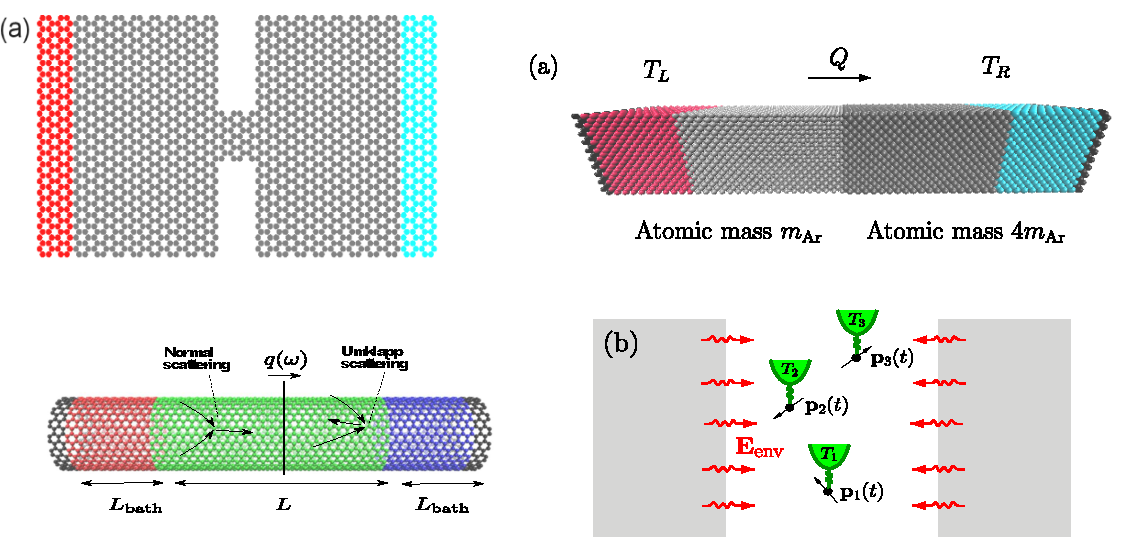
\includegraphics[width=.99\columnwidth]{pics/systems.pdf}
% \caption{Schematic illustration of some of the systems studied in this thesis. (a) Constriction in graphene. (b) Planar interface between two mass-mismatched face-centered cubic lattices. (c) Carbon nanotube. (d) Oscillating dipoles in a cavity.}
%\label{fig:intro_systems}
%\end{center}
%\end{figure}

%Some of the systems studied in this work are illustrated in Fig. \ref{fig:intro_systems}. First, we investigate interference effects and the effect of temperature on energy transfer and non-equilibrium temperature profiles in constrictions in two-dimensional lattices such as graphene, depicted in Fig. \ref{fig:intro_systems}(a). Interference effects are shown to give rise to intricately shaped temperature profiles in small constrictions, with increasing anharmonic scattering washing out the profiles. The work also clarifies the role played by the bulk reservoirs in heat transfer through low-dimensional systems. 

%We develop a computational method to determine the heat current carried by each vibrational frequency and apply the method to investigate the role of anharmonic phonon scattering on the thermal conductance of a planar interface depicted in Fig. \ref{fig:intro_systems}(b). The results show that anharmonic scattering can contribute to interfacial heat transfer both by presenting a dissipation mechanism for evanescent modes localized close to the interface and enabling three-phonon frequency-halving and frequency-doubling energy transfer processes at the interface. The same computational method is used to determine the phonon mean free paths in carbon nanotubes [Fig. \ref{fig:intro_systems}(c)] from non-equilibrium simulations, offering a novel method of determining the non-equilibrium scattering lengths in nanostructures and showing that mean free paths of energy carriers in carbon nanotubes can exceed 10 $\mu$m. In another work, we show that twinning Si nanowires could act as efficient thermoelectric materials due to their small thermal conductivity at a specific twinning period.

%Finally, we present a quantum Langevin equation-based approach on calculating electromagnetic energy transfer rates between oscillating dipoles and apply the theory to investigate the role of an inhomogeneous environment on electromagnetic energy transfer between nanoparticles. In addition to providing a new microscopic theory of electromagnetic energy transfer, we show that the confinement of electromagnetic modes in the mirror cavity [illustrated in Fig. \ref{fig:intro_systems}(d)] gives rise to oscillations in the heat transfer rates between polar nanoparticles as a function of particle distance. Heat transfer rate between nanoparticles is shown to be enhanced also close to a surface supporting surface phonon polaritons.



% Energy transfer between and inside bodies generally occurs by three mechanisms: conduction, radiation and convection \cite{}. 
%The energy transfer generally occurs by three mechanisms: conduction, radiation and convection \cite{}. Thermal conduction, which is the dominant mechanism in solids, is energy transfer inside a given body and occurs through (i) the microscopic interactions between the atoms and molecules constituting the body and, in case of metals, (ii) movement of free electrons. In fluids and gases, energy is transferred not only by conduction but also by the net motion of the energy-carrying molecules themselves, a process known as convection. As an example, the familiar law that hot air rises above the cold air is convection. Finally, energy can be transmitted by electromagnetic waves, i.e., thermal radiation. Unlike conduction and convection, thermal radiation does not require any mediating medium to carry energy: this is best exemplified by the thermal radiation from the Sun.

%The scope of this work is to investigate thermal conduction by lattice vibrations and electrons in nanoscale crystalline solids and thermal radiation between nanoparticles. In crystalline solids, lattice vibrations form propagating collective modes, the quanta of which are known as phonons. Below, we briefly review the main phenomena characteristic of thermal conduction in nanoscale. Detailed theory of lattice dynamics is presented in Chap. XXX.

% when the size of the structure or the scale of observations reaches nanoscale.

%\subsection{Experimental observations of }

%\begin{itemize}
% \item Interference, particles versus waves
% \item Boundaries and interfaces
% \item Ballistic versus diffusive, coherence
%\end{itemize}


\section{Energy transfer in nanoscale systems}
\begin{itemize}
 \item Phonon, photon, electron transport overlap
\end{itemize}
This Section reviews the prominent energy transfer phenomena of nanoscale systems. Vibrational energy transfer is reviewed in Subsection \ref{sec:intro_vib}. Emphasis is placed on the violations of the classical Fourier's law of heat transfer and defining the various length scales emerging in the microscopic scale. The mathematical theory underlying vibrational energy transfer is presented in detail in Chap. \ref{chap:theory}. 

% Because this thesis mainly focuses on phonon and photon transport, more emphasis is placed on these transfer mechanisms. 

Electromagnetic energy transfer phenomena in nanoscale are reviewed in Subsection \ref{sec:intro_em}. In electromagnetic energy transfer, the macroscopic laws of thermal radiation such as Planck's radiation law break down when the separation between bodies becomes similar to the wavelengths of thermally excited electromagnetic fields. At such small separations, evanescent near-fields localized close to the material surfaces can couple the materials and thereby strongly increase energy transfer rates. %The near-field energy transfer is reviewed in Subsection \ref{sec:intro_em}.

Subsection \ref{sec:intro_electrons} reviews electronic conduction of heat in metallic and semi-conducting nanostructures. Because electron transport topics such as electron conductance quantization, Coulomb blockade, localization etc. are outside the scope of this thesis, Subsection \ref{sec:intro_electrons} is only devoted to the discussion of electronic heating in nanostructures. %These effects include the generation of hot spots and the possibility to measure thermal conductivity from local heating. %detrimental electronic heating has been suggested to be reduced by low-dimensional, high thermal conductivity materials

% Hot spots
% Graphene quilts etc.
% Measurement of thermal conductivity from Joule heating 
% Conductance at metal-dielectric interfaces
% Current induced forces?

% Similarity of phonon, photon systems (interference, scattering, Green's function methods,...)

\subsection{Vibrational energy transfer in nanoscale}
\label{sec:intro_vib}
% Start from Peierls's theory
The microscopic theory for thermal conduction was developed by Rudolf Peierls in 1929 \cite{peierls29}. Understanding that collective lattice vibrations (phonons) carry heat in crystalline solids, he proposed that thermal resistivity arises from the scattering of phonons from lattice imperfections and other phonons. These scattering mechanisms existing in any non-ideal material at non-zero temperature give rise to a finite phonon mean free path, characterizing the average distance between scattering events. At length scales much larger than the mean free path, the heat carriers are expected to essentially perform a random walk with constant drift along the temperature gradient and heat transfer is well described by Fourier's local theory. At length scales smaller than the mean free path, on the other hand, phonons can travel without scattering and Fourier's theory must be invalid. 

% Thermal conduction in macroscopic systems is traditionally described using Fourier's law \cite{fourier}, stating that the heat flux at any given point is proportional to the temperature gradient at the same point. The theory leads, however, to the unphysical phenomenon that a local temperature perturbation can propagate infinitely fast \cite{chen}, in direct contradiction to the finiteness of the speed of sound and also special relativity. This indicates that Fourier's theory must ultimately break down in nanoscale.

This expected transition to the Fourier limit in sufficiently large systems has been questioned in recent decades by computer simulations \cite{lepri97,lepri03,mai07,dhar08} and heat transfer experiments \cite{yang10,xu14} indicating that the Fourier limit may never be reached in low-dimensional systems. In one-dimensional oscillator chains, for example, it is now widely accepted \cite{dhar08} that the thermal conductivity diverges as a function of system length following a power-law \cite{mai07}. It is, however, still debated \cite{marconnet13} if any physical system such as a nanowire can be treated as a one-dimensional object and could therefore exhibit the divergence. %Some experiments have claimed to have observed such anomalous thermal conduction in silicon nanowires \cite{yang10}, but the evidence remains inconclusive. % In two-dimensional materials such as graphene, similar divergence is expected, and recent experiments and simulations for graphene have suggested this to be the case \cite{xu14}. %\citepub{cnt}

\begin{figure}
\begin{center}
 %\includegraphics[width=8.6cm]{pics/schwab00_fig3.ps}
 \includegraphics[width=8.6cm]{pics/schwab00_fig3.pdf}
 \caption{Thermal conductance measured as a function of temperature by Schwab \textit{et al.} \cite{schwab00}. In their experimental setup, heat was transferred through four nanowires with four acoustic modes in each carrying the heat. The measured conductance at low temperature is therefore $G=16g_0$, where $g_0$ is the conductance quantum. Reprinted with permission from Ref. \cite{schwab00}.}
\label{fig:intro_schwab}
\end{center}
\end{figure}

In systems smaller than the phonon mean free path, on the other hand, Fourier's law is undisputably invalid due to the scattering-free propagation of heat carriers. Such bullet-like transport of phonons is called ballistic transport, contrasting with the diffusive transport of Fourier-like systems. The most striking example of ballistic transport is the thermal conductance quantization, predicted theoretically by Rego and Kirczenow in 1998 \cite{rego98}. Their calculations showed that at sufficiently low temperatures, where phonon scattering is minimal and only the lowest-frequency phonon modes can be excited, thermal conductance through a narrow constriction is an integer multiple of the thermal conductance quantum. The thermal conductance quantum, which is analogous to the quantum of electrical conductance, is independent of any material properties and only depends on temperature and Planck's constant. The predicted quantization was observed experimentally in 2000 by Schwab \textit{et al.} \cite{schwab00} (see Fig. \ref{fig:intro_schwab}), thereby indirectly confirming also the existence of ballistic transport.

In addition to the mean free path, there is another internal length scale governing heat transfer, the phonon wavelength. In devices smaller than or of the same size as dominant phonon wavelength, interference effects appear. Interference effects have enabled designing acoustic reflectors with novel applications in enhancing the optical-mechanical coupling \cite{fainstein13} and phonon lasing \cite{maryam13}. Wavelength-related effects are also useful in thermal engineering: as an example, Kim \textit{et al.} were able to reduce the thermal conductivity of InGaAs alloy (which naturally scatters short-wavelength phonons due to point defects) by introducing nanoparticles acting as scatterers for mid-to-long-wavelength phonons \cite{kim06}. %\citepub{fpu}\citepub{fpu2}\citepub{gf} % Other examples of interference

In a nanoscale system with relatively long internal phonon mean free paths, the material surfaces and interfaces play an important role in thermal conduction. At rough surfaces, for example, phonons are scattered into all directions, which strongly suppresses the heat flow. The resulting reduced thermal conductivity has been noted to be responsible for the moderately high thermoelectric figure of merit of Si nanowires \cite{hochbaum08}. At material interfaces, the mismatch in the acoustic properties of the materials inevitably scatters phonons.  This contact resistance between dissimilar materials can act as a major bottleneck limiting the extraction of heat from electronic devices, thereby hindering their performance \cite{pop10}. Many methods have been suggested to reduce the thermal resistance between materials, including chemical functionalization \cite{hopkins11,kaur14}, external pressure \cite{shen11,chalopin12}, and heat-mediating thin films \cite{english12}. %\citepub{spectral}\citepub{twinning}

% Relation to the thesis
Concepts such as phonon interference, ballistic transport, mean free paths, and interface scattering appear throughout this thesis. In Publications \cp{fpu}, \cp{fpu2}, and \cp{gf}, we explore the interference effects exhibited in thermal conduction through nanoscale constrictions and reveal intricate interference patterns in local nonequilibrium temperature profiles. We also show how such patterns vanish at higher temperatures due to increased scattering. In Publication \cp{spectral}, we present detailed maps of the contributions of different vibrational frequencies to thermal conduction across a mass-mismatched interface, improving thereby the understanding of heat transfer mechanisms at interfaces and presenting guidelines for future thermal engineering of high-conductance interfaces. Publication \cp{cnt} presents a non-equilibrium method for determining the mean free paths of phonons in carbon nanotubes, supplying a theoretical description of the ballistic-diffusive crossover in one-dimensional systems. In Publication \cp{twinning}, we perform ''thermal engineering'' and demonstrate the existence of minimun thermal conductivity at a certain twinning period length in a silicon nanowire. The minimun arises from the maximal blocking of bulk-like scattering-free propagation of phonons through the nanowire by the periodically repeating twinning boundaries.


%As noted by Kapitza already in 1930s \cite{}, carrier scattering at interfaces between materials also gives rise to thermal resistance. Even in the absence of defects, 

% Point contacts \cite{bartsch12}

% Contact resistance is a bottleneck
% Material properties increasingly dominated by interfaces

% Interfaces

% Superlattices, phonon mirrors

% While there is convincing evidence from numerical simulations that the Fourier limit is always achieved in three-dimensional systems \cite{saito10,wang10}, this seems not to be the case in one- or two-dimensional systems. Numerical simulations \cite{lepri97,mai07} and hydrodynamical theory \cite{} suggest that the thermal conductivity in one-dimensional systems diverges in a power-law fashion as a function of system length, but clear experimental demonstration of the divergence has not been achieved so far. In two-dimensional systems, thermal conductivity is expected to diverge logarithmically \cite{}. Recent experiments claim to have observed the divergence in graphene \cite{xu14}.

%\subsection{Thermal boundary resistance}

%\subsection{Thermal engineering}

\subsection{Electromagnetic energy transfer in the near-field}
\label{sec:intro_em}
Accelerating charges are known to emit electromagnetic radiation \cite{}. Because the electrons and nuclei in any solid material undergo thermal (and quantum) fluctuations, all materials therefore emit electromagnetic radiation carrying heat. In 1900, Max Planck \cite{planck00a} studied the radiation emitted by a blackbody and gave birth not only to quantum theory but also to Planck's blackbody radiation law, which has since been observed to describe, for example, the spectrum of cosmic microwave background radiation at the accuracy of XXX.

Planck's law inherently suggests that the total power of the emitted radiation is independent of the distance from the object. This follows from the assumption that only propagating waves contribute to the energy density. Close to the material surface, solution of Maxwell's equations gives, however, also rise to evanescent electromagnetic fields localized at a distance of a few wavelengths from the object \cite{polder71}. One can then envisage placing another object sufficiently close to the radiating body so that the evanescent fields can induce motion of charges in the added object, leading to energy transfer by the evanescent fields. Planck's law therefore breaks down at very small distances. 

The breakdown in Planck's law was first observed by Hargreaves \cite{hargreaves69}, who found an enhancement in the heat transfer rate between two chromium layers as the layers were separated by subwavelength gap. The theoretical calculation for the exact enhancement rate was carried out by Polder and van Hove \cite{polder71}, and consequently near-field enhancement effects were predicted in numerous geometries \cite{loomis94,pendry99,carminati99,shchegrov00,mulet01,volokitin01}. In the last decade, advances in experimental techniques have allowed for very precise measurements of near-field enhancement rates \cite{}, confirming the experimental predictions. Near-field effects are now routinely used in thermal microscopy \cite{majumdar99,muller-hirsch99,kittel05,kittel08}. They are also expected to give rise to engineering applications in, e.g., infrared thermophotovoltaics \cite{dimatteo01,narayanaswamy03,laroche06} and building narrow-band infrared antennas \cite{greffet02}. 

\begin{figure}
\begin{center}
 %\includegraphics[width=8.6cm]{pics/schwab00_fig3.ps}
 \includegraphics[width=8.6cm]{pics/shchegrov00_fig1.pdf}
 \caption{The spectral energy density of electromagnetic field (arbitrary units) close to a SiC surface at distances of (a) $1$ mm, (b) $2$ $\mu$m, and (c) $100$ nm. At the distance of 100 nm, the spectral energy density is dominated by the surface phonon polariton at frequency $\omega=178.7$ Trad/s, resulting in essentially monochromatic energy emission. Inset show the spectral energy densities plotted in semilogarithmic scale. Reprinted with permission from Ref. \cite{shchegrov00}.}
\label{fig:intro_shchegrov}
\end{center}
\end{figure} 

Near-field effects are particularly strong for materials supporting evanescent surface waves decaying at both sides of the surface \cite{shchegrov00}. The surface waves arise from the coupling between the electromagnetic field and either the free electrons (surface plasmon polaritons) or transverse optical phonons (surface phonon polaritons). While surface plasmon polaritons can only be thermally excited in metals at temperatures much higher than room temperature, surface phonon polaritons can contribute to thermal transfer in polar semiconductors even at room temperature. To demonstrate the large contribution of surface waves, Fig. \ref{fig:intro_shchegrov} shows the theoretically calculated \cite{shchegrov00} spectral energy density of the electromagnetic field at various distances from a SiC surface.

Similarly, near-field effects strongly increase the spectral density of the electromagnetic field in the vicinity of nanoparticles made of a polar material. Consequently, heat transfer between two nanoparticles in vacuum is found to strongly increase at small distances \cite{domingues05}. In practice, however, the required nanoparticle distances for efficient heat transfer may be too small, so for practical applications it would be necessary to engineer the thermal conductance to be higher. From the theory of dipole emission, it is well known that the optical-mechanical coupling can be enhanced by orders of magnitude in an inhomogeneous environment such as in a mirror cavity \cite{novotny}. This raises the question, if the interparticle heat transfer rate between particles could be enhanced by cavity. This question was investigated and answered in positive in \citepub{dipole}.




 %it has a few problems. First, multiple different microscopic definitions for the polarizability exist, varying on whether the polarizability expresses the response, e.g., to the total electric field consisting of the external field and the internal polarization field or only the external field. This ambiguity is related to the observation of Manjavacas and Garc\'ia de Abajo \cite{manjavacas12} that Eq. \eqref{eq:th_fed_fdt} can be used to predict unphysical fluctuations even in a non-absorbing medium. The imaginary part of polarizability must, after all, be strictly positive even in a non-absorbing medium due to the radiation reaction force, but a non-absorbing medium cannot emit radiation.  % Even in a non-absorbing medium, the imaginary part of the polarizability is non-zero due to the radiation reaction force. Therefore, Eq. \eqref{eq:th_fed_fdt} predicts unphysical fluctuations even in absence of actual dissipation.

%A second difficulty in Eq. \eqref{eq:th_fed_fdt} is that it does not simply allow for coupling of, say, acoustic and optical degrees of freedom. 



%Electromagnetic energy transfer between dielectric bodies at different temperatures is commonly described using the fluctuational electrodynamics theory developed by Rytov. The theory describes the radiation generated by thermal motion of charges and its connection to the dissipation captured by the imaginary part of the polarizability. 


%Following theoretical developments and advances in experimental techniques, near-field 
%The theory has since been used to theoretically predict strong near-field enhancements of heat transfer in various geometries \cite{loomis94,pendry99,mulet01,volokitin01}. 

% Surface polaritons

% The theoretical calculation of the exact near-field enhancement was consequently carried out by Polder and van Hove \cite{polder71}, who applied the fluctuational electrodynamics theory developed by Rytov \cite{rytov58}. 



%The predictions have been explored in more detail also experimentally [13-18]. 
\iffalse
Electromagnetic energy transfer between dielectric bodies at different temperatures is commonly described using the fluctuational electrodynamics (FED) approach \cite{joulain05,volokitin07} developed by Rytov \cite{rytov58,rytov} and first applied to condensed matter physics by Lifshitz \cite{lifshitz55,lifshitz56}. According to FED, thermal motion of charged particles in a body creates random currents, which induce electromagnetic fields. Outside the body, the field is then either radiated to free space or absorbed in the near or far-field regime by another body. In the near-field, the heat transfer rate between bodies can surpass the Planckian blackbody limit \cite{planck} by several orders of magnitude, as first suggested theoretically \cite{polder71,pendry99,carminati99,shchegrov00,mulet01,volokitin01} and later confirmed experimentally \cite{kittel05,hu08,rousseau09,shen09,ottens11}. Near-field enhancement of heat transfer is expected to have numerous applications in, e.g., thermal microscopy \cite{majumdar99,muller-hirsch99,kittel05,kittel08}, infrared thermophotovoltaics \cite{dimatteo01,narayanaswamy03,laroche06} and narrow-band infrared antennas \cite{greffet02}.
\fi


%As early as 1884, John Poynting calculated the energy flux carried by propagating electromagnetic waves. 


\iffalse
\section{Summary of experimental techniques}

\subsection{Thermal conductivity}

\begin{itemize}
 \item $3\omega$ technique
 \item Picosecond ultrasonic techniques (transient reflectance)
\end{itemize}

\subsection{Local temperature}

\subsection{Electromagnetic near-field transfer}

\subsection{Scanning thermal microscopy}

Measure the temperature of an AFM probe during the scan using either a thermocouple junction (measure voltage caused by temperature change) or microbolometer technique (measure change in resistance). In the latter, two leads are connected at the end of the probe by a Joule heating element which can be used either for temperature measurement by measuring its temperature change or for heating by driving current through it. In the constant power mode, the resistance of the heating element is measured by measuring the voltage in a Wheatstone bridge. If the voltage is fed back to the contact voltage, one can keep constant temperature at the resistor. 

Heat flow from the tip can be due to
\begin{itemize}
 \item Solid-solid conduction (this is what is wanted)
 \item Liquid-liquid conduction by the liquid meniscus between the tip and the sample, use UHV conditions
 \item Gas-gas conduction, use UHV conditions
 \item Near-field radiation between the tip and the sample
 \item Heat flow to cantilever
\end{itemize}

If the temperature of the tip, say, drops during the scan, this can be due to (a) lower local temperature, or (b) higher thermal conductivity at the sample spot. Also lower heat capacity is possible (?). 

Technique developed by Nonnenmacher (1992), Wickramasinghe (1992), Majumdar (1993), Pilkki (1994), etc.

Other methods to measure temperature are (see the review by Yue and Wang)
\begin{itemize}
 \item Optical methods based on the temperature-dependence of Raman or fluorescence signal of the measuring target (molecule, nanoparticle, etc.), which can also be used as the temperature sensor at the tip of an AFM, for example
 \item Near-field optical temperature measurement, with or without aperture
\end{itemize}

\subsection{Inelastic neutron scattering}
 \begin{itemize}
  \item Neutrons interact strongly only with the atomic nuclei (dipole scattering etc. typically weaker)
  \item Map the change in the neutron energy and momentum, one-phonon scattering processes sharply resolved among the multi-phonon process background
  \item Vary neutron energy, orientation of crystal and detection direction
  \item Gives phonon dispersion relations and broadenings, anharmonic effects mapped recently e.g. in doi:10.1038/nmat3035 and doi:10.1038/nnano.2013.95
 \end{itemize}
\fi


\chapter{Theory and methods}
\label{chap:theory}

Heat transfer is customarily described theoretically either at an atomistic level, monitoring the energy exchanged between individual atoms, or by treating the heat carriers as a gas of particles. While the latter particle picture is highly useful for, e.g., structures too large for atomic scale treatment, the structures considered in this thesis require atomic scale modeling to capture, e.g., the wave nature of energy carriers.

This chapter reviews the microscopic theory and computational methods used in the thesis. Sections \ref{sec:th_eom1} and \ref{sec:th_eom2} present the relevant equations governing phononic, electronic and photonic energy transfer in microscopic scale. To highlight the common features in the modeling of different carriers, we start by postulating the Langevin equations of motion for the three carriers in Sec. \ref{sec:th_eom1}. Carrier-specific details and the derivation of the presented linearized equations are presented in \ref{sec:th_eom2}. 

Langevin theory is used throughout the thesis to model thermal fluctuations and dissipation, and this theory and the fluctuation-dissipation theorem (FDT) are discussed in Sec. \ref{sec:th_langevin}. All calculations in the thesis aim at computing energy flow in the system, so the corresponding definitions of energy currents and their evaluation are reviewed in Sec. \ref{sec:th_currents}. Section \ref{sec:th_currents} also presents the spectral analysis methods developed in Publications \cp{spectral} and \cp{cnt} for determining frequency-wise contributions to interatomic energy transfer. The evaluation of spectral energy current distribution in non-linear systems capturing phonon-phonon scattering requires monitoring dynamical correlations in atomic trajectories. The atomic trajectories are simulated with the classical molecular dynamics (MD) method, presented in Sec. \ref{sec:methods_md}. The limitations of the models used in this thesis are discussed in Sec. \ref{sec:th_limits}.

\section{Langevin equations for phonon, photon and electron systems}
\label{sec:th_eom1}

Langevin equations are a convenient and simple way to describe heat transfer in atomic scale, accounting for both wave dynamics and dissipation in carrier propagation. This section reviews the general features of the Langevin equations of motion governing energy transfer by lattice vibrations, electromagnetic field, and electrons. The presented linearized equations for phononic, photonic and electronic energy transfer originate, respectively, from the works of Bolsterli, Rich and Visscher \cite{bolsterli70}, Rosa, Dalvit and Milonni \cite{rosa10,rosa11}, and Dhar, Shastry and Sen \cite{dhar03,dhar06b}. The simplification obtained by linearization is that it allows for the analytical solution of the equations of motion in terms of the Green's function (GF). The derivation of the linearized equations from more general equations and the precise definitions of parameters are presented in Sec. \ref{sec:th_eom2}. 

\begin{figure}
 \begin{center}
 \end{center}
  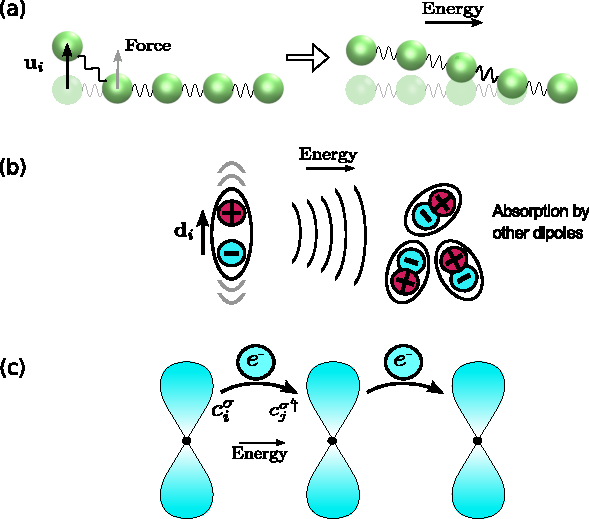
\includegraphics[width=.99\columnwidth]{inkscape/mechanisms.pdf}
 \caption{Schematic illustration of microscopic energy transfer mechanisms: (a) vibrational, (b) electromagnetic, and (c) electronic energy transfer. In phononic transfer, an atom displaced from its equilibrium position exerts a force on the neighboring atoms, giving rise to the propagation of displacement and transfer of energy. Fluctuations in the dipole moment, on the other hand, produce electromagnetic fields carrying energy, which can be absorbed by other dipoles. Electronic energy transfer arises from the hopping of electrons between atomic orbitals, driven by imbalance in electron number or temperature. Electron hopping is mathematically described here by the electron creation and annihilation operators.}
 \label{fig:mechanisms}
\end{figure}

Different energy transfer mechanisms and their corresponding degrees of freedom are schematically illustrated in Fig. \ref{fig:mechanisms}. Vibrational heat transfer in solids arises from the displacements $u_i^{\alpha}$ of each atom $i$ from their equilibrium positions to co-ordinate directions $\alpha\in\{x,y,z\}$. An atom displaced from its equilibrium position exerts a net force on other atoms, thereby leading to the propagation of displacement and transfer of energy. Similarly, electromagnetic energy is generated by fluctuations in local dipole moments $p_i^{\alpha}=qd_i^{\alpha}$, where $q$ is the dipole charge and $d_i^{\alpha}$ the dipole displacement in direction $\alpha$ \cite{rosa10}. The radiated electromagnetic energy propagates according to the Maxwell equations \cite{novotny}, scattered and absorbed by other dipoles. 

Quantum-mechanical electron transport in solids can be intuitively described by the tight-binding model \cite{ashcroftmermin}, in which electrons move by ''hopping'' between electron orbitals localized at individual atoms. Mathematically, the dynamics of a single electron is governed by the one-particle Schr\"odinger equation \cite{griffiths_qm}, but to capture fluctuations and dissipation, it is more practical to formulate the dynamical equations for electron creation and annihilation operators $c_i^{\sigma\dagger}$ and $c_i^{\sigma}$ \cite{ballentine}, which create and annihilate electrons at an orbital $\sigma$ localized at atom $i$, respectively\footnote{Label $\sigma$ is a composite index containing both the orbital wave function and electron spin.}. For notational simplicity, the same lattice subindex $i$ is used for each carrier to label the different spatial degrees of freedom. 

Modeling of energy transfer requires coupling at least some of the degrees of freedom to external reservoirs acting as sources and sinks for energy. With the exception of \citepub{twinning}, where Nos\'e-Hoover thermostats \cite{nose84} are used, we employ Langevin baths as reservoirs in all works included in this thesis. The coupling of an atomic chain to Langevin baths is illustrated by a one-dimensional example in Fig. \ref{fig:langevin_chain}. In this case, the baths serve two purposes: The baths colored in red and blue act as external heat sources and sinks, respectively, and are used to drive energy through the system. The baths colored in green, on the other hand, mimic internal fluctuations and dissipation arising from anharmonic scattering, allowing for capturing non-linear effects in terms of effective relaxation rates \cite{bolsterli70}. This allows for a quantum-mechanical treatment of much larger systems than the more rigourous but computationally heavy Keldysh GF method \cite{haugjauho}, as discussed in more detail in \citepub{gf}. 

\begin{figure}
 \begin{center}
 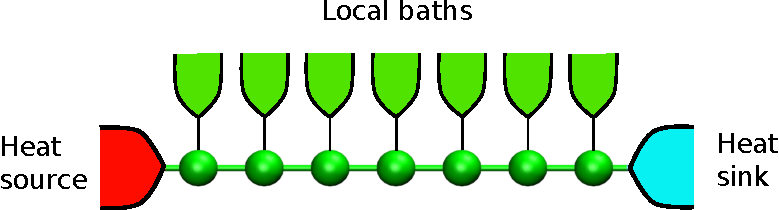
\includegraphics[width=.99\columnwidth]{inkscape/chain_baths.pdf}
 \caption{Schematic illustration of a chain of atoms coupled to Langevin baths. The baths at the left and right boundaries (red and blue) are at different temperatures and act as a heat source and sink, respectively. The baths colored in green describe internal fluctuations and dissipation arising from, e.g., phonon-phonon scattering.}
 \label{fig:langevin_chain}
  \end{center}
\end{figure}

\subsection{Equations of motion: common features}
\label{sec:th_eom}

The equations of motion for the three degrees of freedom $\bu_i$, $\bb{d}_i$, and $c_i^{\sigma}$ are all connected through the Langevin physics describing fluctuations and dissipation, leading to a similar solution method and phenomenology despite involving different energy carriers. The equations read  \cite{bolsterli70,rosa10,rosa11,dhar03}
\begin{subequations}
\begin{align}
 m_i \ddot{\bu}_i(t) &=  - \sum_j \bb{K}_{ij}\bb{u}_j(t) + \xi_i(t) - m_i \gamma \dot{\bu}_i, \label{eq:th_eom1} \\
 m_i \ddot{\bb{d}}_i(t) &= - \sum_j \bb{K}_{ij} \bb{d}_j(t) +q\sum_{j} \bb{E}_{ij}(t)+\xi_i(t)+ q\Eenv(\br_i,t) - m_i \gamma \dot{\bd}_i(t), \label{eq:th_eom2}\\
 i\hbar \dot{c}_i^{\sigma}(t) &= -\sum_{j,\sigma'} t_{ij}^{\sigma\sigma'} c_j^{\sigma'}(t) +\eta_i^{\sigma}(t) - i\hbar \gamma_e c_i^{\sigma}(t) \label{eq:th_eom3}.
\end{align}
\end{subequations}
Here $\bu_i=[u_i^{x},u_i^y,u_i^z]^T$ and $\bd_i=[d_i^x,d_i^y,d_i^z]^T$ are written as three-dimensional vectors. Equations \eqref{eq:th_eom1}, \eqref{eq:th_eom2} and \eqref{eq:th_eom3} contain, generally speaking, four different kinds of parameters: inertial mass $m_i$ of atom or dipole $i$, coupling coefficients $\bb{K}_{ij}$, $\bE_{ij}$ and $t_{ij}^{\sigma\sigma'}$ coupling different degrees of freedom, Langevin noise terms $\xi_i$, $\Eenv$, and $\eta_i$ responsible for thermal fluctuations, and damping coefficients $\gamma$ and $\gamma_e$ accompanying the fluctuations according to the FDT (Sec. \ref{sec:th_langevin}). Noise terms $\xi_i$, $\Eenv$, and $\eta_i$ essentially describe thermal fluctuations in phonon, photon or electron number and are governed either by Bose-Einstein or Fermi-Dirac statistics as detailed in Sec. \ref{sec:th_langevin}. %The stochastic background field $\Eenv(\br_i,t)$ appearing in the dipole equation of motion \eqref{eq:th_eom3} and arising from the thermal fluctuations of the environment ensures balance between electromagnetic absorption and emission in thermal equilibrium \cite{rosa10}.

Equations \eqref{eq:th_eom1}, \eqref{eq:th_eom2} and \eqref{eq:th_eom3} are derived in more detail in Sec. \ref{sec:th_eom2}, but they can be easily understood intuitively. As an example, Eq. \eqref{eq:th_eom1} declares that the acceleration of atom $i$ is proportional to the sum of (i) the forces exerted by other atoms $j$, proportional for each atom pair $i,j$ to the force constant matrix $\bb{K}_{ij}$ calculated from interatomic potential energy, (ii) stochastic Langevin force $\xi_i$ modeling local thermal fluctuations, and (iii) friction term $m_i \gamma \dot{\bu}_i$ responsible for energy dissipation at rate $\gamma$. To highlight the similarities between different carriers, we have used the linear approximation for the interparticle force in equation \eqref{eq:th_eom1}, allowing for the direct solution of the equations of motion as shown in the following Subsection. This assumption is relaxed in Sec. \ref{sec:th_eom2} to allow for more exact treatment of non-linear forces, which are responsible for microscopic phonon-phonon interactions and therefore necessary in the calculation of, e.g., frequency-dependent mean free paths (\citepub{cnt}) and the thermal conductivity of twinning nanowires (\citepub{twinning}). 

It is worth noting that whereas equations \eqref{eq:th_eom1} and \eqref{eq:th_eom2} are purely real and involve second time-derivatives on the left-hand side, Eq. \eqref{eq:th_eom3} for the electron annihilation operator $c_i^{\sigma}$ is imaginary and involves only a single time-derivative. This difference is rooted in the fundamental property of quantum mechanics that time evolution is modeled by diffusion equation in imaginary time (Schr\"odinger equation), allowing for wave-like solutions in real time \cite{ballentine}.

\subsection{Solution of the Langevin equations in terms of Green's functions}
\label{sec:th_eom_solution}
The similarity of Eqs. \eqref{eq:th_eom1}, \eqref{eq:th_eom2}, and \eqref{eq:th_eom3} allows for solving the equations in a similar fashion. The differential equations are first turned into algebraic equations by Fourier transforming the equations\footnote{We define Fourier transformation $\tilde f(\omega)$ for any function $f(t)$, as usual, as
\begin{equation}
 \tilde f(\omega) = \int_{-\infty}^{\infty} dt e^{i\omega t} f(t) \label{eq:th_fourier}
\end{equation}
and the corresponding inverse transformation as
\begin{equation}
 f(t) = \int_{-\infty}^{\infty} \frac{d\omega}{2\pi} e^{-i\omega t}\tilde f(\omega). \label{eq:th_fourier_inv}
\end{equation}}.
With small rearrangement, one then gets three linear systems of equations:
\begin{subequations}
\begin{align}
   - & \sum_{j,\beta}  [m_i (\omega^2+i\gamma \omega) \delta_{ij}\delta_{\alpha\beta} - K_{ij}^{\alpha\beta}] \tilde{u}_j^{\beta}(\omega) = \tilde \xi_i^{\alpha}(\omega) \label{eq:th_eom_fourier_phonon} \\
  - &  \sum_{j,\beta} \left[m(\omega^2+i\gamma\omega) \delta_{ij}\delta_{\alpha\beta} - K_{ij}^{\alpha\beta} +q^2 \omega^2 \mu_0 \mathbb{G}^{\alpha\beta}(\br_i,\br_j;\omega) \right]\tilde{d}_j^{\beta}(\omega) \notag \\
  & \qquad = q\tilde{E}_{\textrm{env}}^{\alpha}(\br_i,\omega) + \tilde{\xi}^{\alpha}_i(\omega) \label{eq:th_eom_fourier_photon} \\ 
  &  \sum_{j,\sigma'} \left[\hbar (\omega+i\gamma_e) \delta_{ij}\delta_{\sigma\sigma'} + t_{ij}^{\sigma\sigma'} \right] \tilde c_j^{\sigma'}(\omega) = \tilde \eta_i^{\sigma}(\omega)  ,  \label{eq:th_eom_fourier_electron}
\end{align}
\end{subequations}
where the Fourier-transformed degrees of freedom and Langevin noise terms are marked by using a tilde as an overscore. Angular frequency is denoted by $\omega$, Kronecker symbol $\delta_{ij}$ is zero for $i\neq j$ and equal to unity for $i=j$, and the co-ordinate directions $\alpha,\beta \in \{x,y,z\}$ are written explicitly in Eqs. \eqref{eq:th_eom_fourier_phonon} and \eqref{eq:th_eom_fourier_photon}. In Eq. \eqref{eq:th_eom_fourier_photon}, the Fourier transform $\tilde{\bE}_{ij}(\omega)$ of the electric field $\bE_{ij}$ appearing in Eq. \eqref{eq:th_eom2} is written in terms of the the electromagnetic Green's dyadic $\mathbb{G}^{\alpha\beta}(\br_i,\br_j;\omega)$ as \cite{novotny}
\begin{equation}
 \tilde{E}_{ij}^{\alpha}(\omega) = q\omega^2 \mu_0 \sum_{\beta} \mathbb{G}^{\alpha\beta}(\br_i,\br_j;\omega)\tilde{d}_j^{\beta}(\omega), \label{eq:th_Eij}
\end{equation}
where $\mu_0$ is the vacuum permeability. The Green's dyadic $\mathbb{G}^{\alpha\beta}(\br_i,\br_j;\omega)$ is defined in Sec. \ref{sec:th_eom2_photon}. 

The linear systems of equations \eqref{eq:th_eom_fourier_phonon}, \eqref{eq:th_eom_fourier_photon} and \eqref{eq:th_eom_fourier_electron} can be written in matrix form by combining all degrees of freedom into single composite vectors by defining $\tilde{\bu}(\omega)=[\tilde u_1^x(\omega),\tilde u_1^y(\omega),\tilde u_1^z(\omega),\tilde u_2^x(\omega),\tilde u_2^y(\omega),\tilde u_2^z(\omega),\dots]^T$ and defining vectors $\tilde{\bd}(\omega)$ and $\tilde{\bb{c}}(\omega)$ similarly. The Langevin terms appearing on the right-hand sides of Eqs. \eqref{eq:th_eom_fourier_phonon}, \eqref{eq:th_eom_fourier_photon} and \eqref{eq:th_eom_fourier_electron} can be similarly written in vector form by accounting for the contribution of each bath $J$ on each degree of freedom. The bath label $J$ corresponds to either local baths, which contribute to the fluctuating force only at a single site, or the environment field $\tilde{E}_{\textrm{env}}^{\alpha}(\br,\omega)$. More details of the labeling are given, e.g., in \citepub{gf}.

Following such a procedure, each of the equations \eqref{eq:th_eom_fourier_phonon}, \eqref{eq:th_eom_fourier_photon}, and \eqref{eq:th_eom_fourier_electron} can be written in the matrix form
\begin{equation}
 \bb{A}(\omega) \tilde{\bb{x}}(\omega) = \sum_J \tilde \zeta^J(\omega). \label{eq:th_general}
\end{equation}
where $\bb{A}(\omega)$ is a coefficient matrix multiplying the degrees of freedom $\tilde{\bb{x}}(\omega)$ (standing for $\tilde{\bu}(\omega)$, $\tilde{\bb{c}}(\omega)$, or $\tilde{\bb{d}}(\omega)$ written in vector form) in Eqs. \eqref{eq:th_eom_fourier_phonon}, \eqref{eq:th_eom_fourier_photon}, and \eqref{eq:th_eom_fourier_electron}. The coefficient matrix $\bb{A}(\omega)$ captures all physical details of the system's deterministic dynamics, including coupling between different degrees of freedom and dissipation arising from the baths. The right-hand side of Eq. \eqref{eq:th_general} is the sum over stochastic Langevin force contributions $\zeta^J$ (standing for $\xi$, $\eta$, or $\Eenv$) from each bath $J$ as discussed above.  

Equation \eqref{eq:th_general} can be solved by defining the GF as the matrix inverse $\bb{G}(\omega)=\bb{A}(\omega)^{-1}$ so that  
\begin{equation}
 \tilde{\bb{x}}(\omega)  =  \bb{G}(\omega) \sum_J \tilde \zeta^J(\omega). \label{eq:th_gf_solution}
\end{equation}
Equation \eqref{eq:th_gf_solution} can be straightforwardly interpreted: system's dynamics at each frequency is defined by the stochastic fluctuations from each bath at the same frequency, with the GF acting as the ''transfer matrix''. Our discrete formulation of the equations of motion allows for writing the GF as a matrix, but corresponding formulation for continuous medium would turn the GF into a function of two continous variables $\br$, $\br'$. In this case, matrix sums in Eqs. \eqref{eq:th_general} and \eqref{eq:th_gf_solution} would be replaced by an integral.

The matrix GF $\bb{G}(\omega)$ is generally of the form \cite{datta}
\begin{equation}
 \bb{G}(\omega) = \left[\bb{G}^0(\omega)^{-1} - \sum_J \Sigma^J(\omega) \right]^{-1},
\end{equation}
where $\bb{G}^0(\omega)$ is the GF in absence of dissipation (i.e., Langevin baths) and bath self-energy matrices $\Sigma^J(\omega)$ describe the dissipation and energy level renormalization arising from the interaction with each bath $J$. For example, the self-energy corresponding to the bath at site $k$, introducing a friction term $m_i\gamma \dot{\bu}_k$ in the equation of motion for $\bu_k$, is $[\Sigma(\omega)]_{ij}=-im_i\gamma \omega \delta_{ij} \delta_{ik}\unitdyadic$. Here $\unitdyadic$ is the $3\times3$ unit matrix. 

With the FDT for the force variances $\langle \zeta^J(\omega) \zeta^J(\omega')^T \rangle$ presented in Sec. \ref{sec:th_langevin} and the solution \eqref{eq:th_gf_solution} available, one can calculate the thermal averages of any observable of interest. The calculation of heat current $ Q_i^{\textrm{bath}}$ to bath $i$, which represents the locally dissipated power, leads to a Landauer-B\"uttiker-like expression \cite{landauer57,buttiker92} as outlined in Sec. \ref{sec:th_currents} and shown in detail in \citepub{gf}. 

\section{Equations of motion: Carrier-specific details}
\label{sec:th_eom2}

\subsection{Phonons}

\label{sec:th_eom2_phonon}

We now move on to carrier-specific details leading to the linear Langevin equations \eqref{eq:th_eom1}, \eqref{eq:th_eom2}, and \eqref{eq:th_eom3}, starting from phonon heat transfer. The general equations of motion governing lattice dynamics are dictated by the lattice Hamiltonian \cite{ziman}
\begin{equation}
 \ca{H}_{\textrm{ph}} = \sum_{i=1}^N \frac{(\bp^{\textrm{kin}}_i)^2}{2m_i} + \ca{V}(\bb{r}_1,\dots,\bb{r}_N). \label{eq:th_hamiltonian}
\end{equation}
Here $\br_i$, $\bp^{\textrm{kin}}_i$, and $m_i$ are the position, kinetic momentum and mass of atom $i$, respectively. The total number of atoms (which can also be infinite) is denoted by $N$. The first term of Eq. \eqref{eq:th_hamiltonian} is the total kinetic energy of the atoms and the second term $\ca{V}$ is the interatomic potential energy responsible for the interatomic interactions. The choice of the potential energy function $\ca{V}$ is crucial for an accurate description of the lattice dynamics and, consequently, of energy transfer. In this thesis, we employed the Lennard-Jones \cite{allentildesley}, Tersoff \cite{tersoff88a}, Stillinger-Weber \cite{stillinger85}, and Fermi-Pasta-Ulam \cite{fermi55} potentials for modeling interatomic interactions in different systems.  

Applying Hamilton's equations of motion $\dot{\br}_i=\partial \ca{H}_{\textrm{ph}}/\partial \bp_i^{\textrm{kin}}$ and $\dot{\bp}_i^{\textrm{kin}}=-\partial \ca{H}_{\textrm{ph}}/\partial \br_i$ \cite{fetter} accompanied by stochastic Langevin terms \cite{dhar06} gives the equations of motion
\begin{equation}
 m_i \ddot{\br}_i(t) = \bb{F}_i(t) + \xi_i(t) - m_i \gamma \dot{\bb{r}}_i(t), \label{eq:th_eom}
\end{equation}
where the deterministic force acting on atom $i$ is
\begin{equation}
 \bb{F}_i = - \frac{\partial \ca{V}}{\partial \bb{r}_i}. \label{eq:th_force}
\end{equation}
As discussed in Sec. \ref{sec:th_eom}, the Langevin terms $\xi_i$ and $m_i\gamma \dot{\bb{r}}_i$ generally have two roles in the modeling of heat transfer. They are used both for (i) coupling atoms located at system's boundaries to external heat sources and sinks,  and (ii) to describe dissipative processes, if non-linear interactions accounting for phonon-phonon interactions are neglected. The form of the friction term $m_i \gamma \dot{\bb{r}}_i(t)$, proportional only to instantaneous velocity, is called Ohmic due to its analogoue with a resistor in an electrical circuit \cite{weiss}. In general, the friction term is a time convolution giving rise to frequency-dependent damping \cite{weiss}, but in all publications included in this thesis, only the Ohmic form is used due to its simplicity.
 
Equation \eqref{eq:th_eom} generally describes the motions of atoms and molecules in solid, gas, and liquid systems. In solids, the atoms vibrate close to their equilibrium positions $\br_i^0$ and one can gain more insight into the lattice dynamics by focusing on the regime with small displacements from the equilibrium. The equilibrium positions $\br_i^0$ are defined by the condition of zero force on each atom:
\begin{equation}
 \left. \frac{\partial \ca{V}}{\partial \br_i} \right|_{\br_j=\br_j^0 \forall j} = 0. \label{eq:th_zeroforce}
\end{equation}
Assuming that the atoms remain close to the equilibrium positions, one can expand the potential energy in Taylor series in terms of the displacements $\bu_i=\br_i-\br_i^0$ \cite{ziman}:
\begin{equation}
 \ca{V} = \ca{V}_0 + \frac{1}{2} \sum_{i,j} \sum_{\alpha,\beta} u_i^{\alpha} K_{ij}^{\alpha \beta} u_j^{\beta}  + \frac{1}{6} \sum_{i,j,k} \sum_{\alpha,\beta,\gamma} \Upsilon_{ijk}^{\alpha\beta\gamma}  u_i^{\alpha} u_j^{\beta} u_k^{\gamma} + \mathcal{O}(u^4). \label{eq:th_V_taylor} % B_{ijk}^{\alpha\beta\gamma}
\end{equation}
In contrast to Eq. \eqref{eq:th_eom}, the Cartesian coordinate directions $\alpha,\beta \in \{x,y,z\}$ have been written here explicitly. The constant term $\ca{V}_0$ in Eq. \eqref{eq:th_V_taylor} does not play a role in dynamics, the first-order derivative term is zero due to Eq. \eqref{eq:th_zeroforce}, and the second-order term is proportional to the harmonic force constant (or ''spring'' constant) \cite{ziman}
\begin{equation}
 K_{ij}^{\alpha\beta} = \left. \frac{\partial^2 \ca{V}}{\partial u_i^{\alpha} \partial u_j^{\beta}} \right|_{\bu=\mathbf{0}}. \label{eq:th_K_def}
\end{equation}
The third term on the right-hand side of Eq. \eqref{eq:th_V_taylor} is proportional to the first-order anharmonic force constants
\begin{equation}
 \Upsilon_{ijk}^{\alpha\beta\gamma} = \left. \frac{\partial^3 \ca{V}}{\partial u_i^{\alpha} \partial u_j^{\beta} \partial u_k^{\gamma}} \right|_{\bu=\mathbf{0}}.
\end{equation}
The first and higher-order anharmonic terms correspond to phonon-phonon interactions \cite{ziman} responsible for anharmonic scattering. First-principles calculation of thermal conductivities and phonon mean free paths requires explicitly including these terms in the equations of motion. The non-linearity of the resulting equations prevents, however, their direct solution, so one needs to turn either to computationally heavy Keldysh GF techniques \cite{wang08} or simulating lattice dynamics using the classical MD method \cite{allentildesley}. MD is used in Publications \cp{spectral}, \cp{cnt}, \cp{twinning}, \cp{fpu}, and \cp{fpu2} due to its flexibility and applicability to large system sizes. MD is reviewed in Sec. \ref{sec:methods_md}.

At sufficiently low temperatures or when dissipative events can be modeled in terms of a given relaxation time, anharmonic terms can be neglected. Including only the two first terms in the right-hand side of Eq. \eqref{eq:th_V_taylor} in the equation of motion \eqref{eq:th_eom} for the atomic displacement $\bu_i=\br_i-\br_i^0$ gives the system of linear equations \eqref{eq:th_eom1}, repeated here for convenience:
\begin{equation}
 m_i \ddot{\bu}_i(t) =  - \sum_j \bb{K}_{ij}\bb{u}_j(t) + \xi_i(t) - m_i \gamma \dot{\bu}_i.  \tag{\ref{eq:th_eom1}}
\end{equation}
The linearity of Eq. \eqref{eq:th_eom1} allows for direct solution in frequency domain as discussed in Sec. \ref{sec:th_eom_solution} and, consequently, including quantum statistics through the quantum FDT for the noise terms $\xi_i$ (Sec. \ref{sec:th_langevin}). 

\subsection{Photons}
\label{sec:th_eom2_photon}
Energy transfer by electromagnetic waves is described by the Maxwell equations \cite{jackson}. In the non-magnetic materials with no free charges as considered in this work, the electromagnetic fields arise from the fluctuating electric polarization fields inside the bodies, and the Maxwell equations for the electric field $\bE(\br,t)$ and magnetic field $\bb{H}(\br,t)$ read \cite{novotny}
\begin{subequations}
\begin{align}
  \nabla \times \bE(\br,t) + \mu_0 \frac{\partial \bb{H}(\br,t)}{\partial t} &= 0 , \label{eq:th_maxwell1} \\
  \nabla \times \bb{H}(\br,t) - \varepsilon_0 \frac{\partial \bb{E}(\br,t)}{\partial t} &=  \bb{j}(\br,t) , \label{eq:th_maxwell2} \\
   \nabla \cdot \bb{H}(\br,t) &= 0, \\
   \varepsilon_0 \nabla \cdot  \bb{E}(\br,t) &= -\nabla \cdot \bb{P}(\br,t).
\end{align}
\end{subequations}
Here, $\mu_0$ and $\varepsilon_0$ are the magnetic permeability and permittivity of vacuum, respectively. The polarization current $\bb{j}(\br,t)=\partial \bb{P}(\br,t)/\partial t$ defined in terms of the polarization density $\bb{P}(\br,t)$ appears as a source term in Eq. \eqref{eq:th_maxwell2}, giving rise to an electromagnetic field according to Eqs. \eqref{eq:th_maxwell1} and \eqref{eq:th_maxwell2}. The radiated electromagnetic field carries an energy flux, whose magnitude and direction are given by the Poynting vector $\bb{S}(\br,t)=\bb{E}(\br,t)\times \bb{H}(\br,t)$ \cite{novotny}. The polarization density consists of stochastic and electrically induced contributions \cite{benabdallah11} as discussed below. 

To derive an equation of motion for the electric field alone, we calculate the curl of Eq. \eqref{eq:th_maxwell1}:
\begin{alignat}{2}
  \nabla \times \nabla \times \bE(\br,t) &= - \mu_0 \frac{\partial}{\partial t} \left[\nabla \times \bb{H}(\br,t) \right] .
\end{alignat}
By using Eq. \eqref{eq:th_maxwell2}, we get the Helmholtz equation for the electric field \cite{novotny}:
\begin{equation}
   \nabla \times \nabla \times \bE(\br,t) + \mu_0 \varepsilon_0 \frac{\partial ^2\bb{E}(\br,t)}{\partial t^2}=  - \mu_0 \frac{\partial^2 \bb{P}(\br,t)}{\partial t^2}. \label{eq:th_eom_photons} % \label{eq:th_curlcurlE}
\end{equation}

To separate the fluctuating terms in the polarization density $\bb{P}(\br,t)$ in Eq. \eqref{eq:th_eom_photons}, we divide the polarization density into the induced and fluctuating parts as $\bb{P}(\br,t)=\bb{P}_{\textrm{ind}}(\br,t)+ \bb{P}_{\textrm{fluc}}(\br,t)$ \cite{benabdallah11}. In the linear and local approximation, the induced part is proportional to the electric field in the frequency domain \cite{novotny}:
\begin{equation}
 \tilde{\bb{P}}_{\textrm{ind}}(\br,\omega)= \varepsilon_0 \chi(\br,\omega) \tilde{\bb{E}}(\br,\omega), \label{eq:th_P_chi}
\end{equation}
where $\chi(\br,\omega)$ is the susceptibility. The imaginary part of $\chi(\br,\omega)$ is responsible for dielectric losses \cite{jackson}. The fluctuating polarization density $\bb{P}_{\textrm{fluc}}(\br,t)$ is the analogue of the Langevin force and its variance in frequency-domain is proportional to the imaginary part of $\chi(\br,\omega)$ through the FDT presented in Sec. \ref{sec:th_langevin}.

Equation \eqref{eq:th_P_chi} lumps the complex response of the medium to the local electric field into a single, macroscopic parameter $\chi(\br,\omega)$. While such a macroscopic description has been used with great success to model energy transfer by electromagnetic fields in the framework of fluctuational electrodynamics \cite{rytov} (see, e.g., Refs. \cite{volokitin07} and \cite{joulain05} for reviews), it is expected to break down in nanoscale \cite{chalopin12b}. 

A more microscopic model for fluctuating polarization fields was introduced by Rosa \textit{et al.} \cite{rosa10,rosa11} for the purpose of quantizing electromagnetic fields in lossy media. They modeled the polarization as a collection of dipoles $\bp_i$ located at points $\br_i$, corresponding to the dipole density
\begin{equation}
 \bb{P}(\br,t) = \sum_i \bp_i(t) \delta(\br-\br_i).
\end{equation}
The dynamics of each dipole was modeled by the classical oscillator model with mass $m_i$ and resonance angular frequency $\omega_0$ so that the Langevin equation of motion for the dipole displacement $\bd_i=\bp_i/q$ reproduces Eq. \eqref{eq:th_eom2} (with $K_{ij}^{\alpha\beta}=m\omega_0^2\delta_{ij}\delta_{\alpha\beta}$): \cite{rosa10,rosa11}
\begin{equation}
 m_i \ddot{\bb{d}}_i(t) = - m \omega_0^2 \bb{d}_i(t) +q\sum_{j} \bb{E}_{ij}(t)+\xi_i(t)+ q\Eenv(\br_i,t) - m_i \gamma \dot{\bd}_i(t). \label{eq:th_eom2b}
\end{equation}
The stochastic Langeving force $\xi_i$ and friction $m_i\gamma \dot{\bd}_i$ account for mechanical fluctuations and dissipation in dipole dynamics, respectively, and are equivalent to the corresponding Langevin terms in the phonon equation of motion \eqref{eq:th_eom}. The thermal background field $\Eenv(\br_i,t)$ acts as a similar noise term, corresponding to electromagnetic absorption of energy from the radiation field. To ensure balance between electromagnetic absorption and emission in thermal equilibrium, there must be an accompanying dissipative term in the equation of motion. Such a term is found in the local field $\bE_{ii}$, which manifests as Abraham-Lorentz radiation damping in the dipole motion \cite{jackson} as discussed in more detail in \citepub{dipole}. 

The local electric field $\bE_{ij}$ acting as a force term in Eq. \eqref{eq:th_eom2} and coupling different dipoles can be written in frequency-domain as [Eq. \eqref{eq:th_Eij}] \cite{novotny,rosa11}:
\begin{equation}
 %\tilde \bE(\br,\omega) = \tilde \bE_0(\br,\omega) + i \omega \mu_0 \int_V d\mathbf{r}' \mathbb{G}(\br,\br';\omega) \tilde{\bb{j}}(\br',\omega). \label{eq:th_Etilde}
\tilde \bE_{ij}(\omega) = \omega^2 \mu_0 \mathbb{G}(\br_i,\br_j;\omega) \tilde{\bb{p}}_j(\omega), \tag{\ref{eq:th_Eij}}
\end{equation}
where $\mathbb{G}(\br,\br';\omega)$ is the electromagnetic Green's dyadic found by solving Eq. \eqref{eq:th_eom_photons} in frequency-domain for a point-like dipole at $\br'$ \cite{novotny}:
 \begin{equation}
 \nabla \times \nabla \times \gem(\bb{r},\br';\omega) - (\omega^2/c^2) \epsenv(\br,\omega)\gem(\bb{r},\br';\omega)  =  \delta(\bb{r}-\br')\unitdyadic. \label{eq:intro_gemdef}
\end{equation}
For generality, we have assumed that the point-like dipole is located in an inhomogeneous environment with dielectric constant $\epsenv(\br,\omega)$ to allow for modeling dipole-dipole energy transfer in a mirror cavity as in \citepub{dipole}. The calculation of Green's dyadics for planar multilayer geometries has been presented by Toma\v{s} \cite{tomas95}. By Fourier transforming Eq. \eqref{eq:th_eom2}, substituting Eq. \eqref{eq:th_Eij} and rearranging one gets the linear system of equations corresponding to Eq. \eqref{eq:th_eom_fourier_photon} for the dipole displacements:
\begin{alignat}{2}
 - & \sum_{j,\beta} \left[m(\omega^2-\omega_0^2+i\gamma\omega) \delta_{ij}\delta_{\alpha\beta} +q^2 \omega^2 \mu_0 \mathbb{G}^{\alpha\beta}(\br_i,\br_j;\omega) \right]\tilde{d}_j^{\beta}(\omega) \notag \\
  & \qquad = q\tilde{E}_{\textrm{env}}^{\alpha}(\br_i,\omega) + \tilde{\xi}^{\alpha}_i(\omega). \label{eq:th_eom_fourier_photon_b}
\end{alignat}

While Eq. \eqref{eq:th_eom_fourier_photon_b} is very similar to the corresponding (linearized) equation \eqref{eq:th_eom_fourier_phonon} for phonon heat transfer, there are some differences. In contrast to the static interatomic force constants $K_{ij}^{\alpha\beta}$ appearing in the phonon equation of motion, the dipole-dipole coupling coefficients $\mathbb{G}^{\alpha\beta}(\br_i,\br_j;\omega)$ are (i) frequency-dependent and (ii) depend on the electromagnetic environment through the dielectric constant $\epsenv(\br,\omega)$. The dipole-dipole coupling coefficients $\mathbb{G}^{\alpha\beta}(\br_i,\br_j;\omega)$ can also be very long-ranged, allowing for energy transfer across large distances even in vacuum. These differences between phononic and photonic energy transfer are, however, related to our somewhat artificial separation between lattice vibrations and electromagnetic field. A fully coupled model of lattice vibrations and electromagnetic field \cite{chiloyan15} enables, e.g., tunneling of acoustic phonon energy across vacuum \cite{prunnila10}.

\subsection{Electrons}
\label{sec:th_eom2_electron}

First-principles modeling of electron transport starts from the quantum-mechanical Hamiltonian $\ca{H}_{\textrm{el}}$ for electrons and ions constituting the atomic lattice \cite{ashcroftmermin}. For the simplicity of discussion, we exclude electron-electron, electron-phonon, and electron-photon interactions so that the single-particle Hamiltonian for an electron moving in the (static) potential generated by the ions located at points $\bb{R}_i$ is \cite{ashcroftmermin}
\begin{equation}
 \ca{H}_{\textrm{el}} = - \frac{\hbar^2}{2m_e} \nabla^2  + \sum_i V(\br-\bb{R}_i), \label{eq:th_Hel}
\end{equation}
where $m_e$ is the electron mass and $V(\br-\bb{R}_i)$ is the electrostatic potential from ion $i$. To arrive at the tight-binding approximation, we first solve the eigenstates $\phi_i^{\sigma}$ and the corresponding eigenenergies $E_i^{\sigma}$ for a \textit{single} ion:
\begin{equation}
 \left[ - \frac{\hbar^2}{2m_e} \nabla^2  +  V(\br-\bb{R}_i) \right] \phi_i^{\sigma} (\br) = E_i^{\sigma} \phi_i^{\sigma}(\br). \label{eq:th_schrode}
\end{equation}
Here the eigenstates are labeled by the superscript $\sigma$. The localized solutions of Eq. \eqref{eq:th_schrode} are centered around $\bb{R}_i$ due to the attractive ion potential $V(\br-\bb{R}_i)$. The tight-binding approximation is to assume that the localized orbitals $\phi_i^{\sigma}$ for each atom $i$ form a complete set \footnote{Typically only a small subset is used, as tightly bound states do not need to be included. More generally, Wannier functions can be used as basis functions \cite{ashcroftmermin}.} so that the electron eigenstates of Hamiltonian \eqref{eq:th_Hel} can be written as
\begin{equation}
 \psi(\br) = \sum_{i,\sigma} b_i^{\sigma} \phi_{i}^{\sigma}(\br).
\end{equation}
The Hamiltonian matrix elements of the basis functions are
\begin{alignat}{2}
 \langle \phi_i^{\sigma} | \ca{H}_{\textrm{el}} | \phi_j^{\sigma'} \rangle &= \left\langle \phi_i^{\sigma} \left| - \frac{\hbar^2}{2m_e} \nabla^2  +V(\br-\bb{R}_i)+ \sum_{k\neq i} V(\br-\bb{R}_k) \right |\phi_j^{\sigma'} \right\rangle \\
 &= E_i^{\sigma} \langle \phi_i^{\sigma}|\phi_j^{\sigma'} \rangle + \left\langle \phi_i^{\sigma} \left| \sum_{k\neq i} V(\br-\bb{R}_k) \right| \phi_j^{\sigma'} \right\rangle \label{eq:th_Helements1} \\
  & = E_i^{\sigma} \langle \phi_i^{\sigma}|\phi_j^{\sigma'} \rangle  - \tilde t_{ij}^{\sigma\sigma'}, \label{eq:th_Helements}
\end{alignat}
where we used Eq. \eqref{eq:th_schrode} in Eq. \eqref{eq:th_Helements1} and also defined the ''hopping'' matrix element as 
\begin{equation}
  \tilde t_{ij}^{\sigma\sigma'} = - \int d\bb{r} \phi_i^{\sigma}(\br)^*  \sum_{k\neq i} V(\br-\bb{R}_k)   \phi_j^{\sigma'}(\br).
\end{equation}
Assuming for simplicity that the overlap matrix element $\langle \phi_i^{\sigma}| \phi_j^{\sigma'} \rangle$ is small for $i\neq j$ so that the orbitals form an orthogonal basis, one can write the tight-binding Hamiltonian corresponding to the matrix elements of Eq. \eqref{eq:th_Helements} in the braket notation \cite{schwabl} as 
\begin{equation}
 \ca{H}_{\textrm{el}}^{\textrm{tb}} = \sum_{i,j} \sum_{\sigma,\sigma'} (E_i^{\sigma} \delta_{ij}\delta_{\sigma\sigma'}  - \tilde t_{ij}^{\sigma\sigma'})|\phi_i^{\sigma} \rangle \langle \phi_j^{\sigma'} | . \label{eq:th_Hel_tb}
\end{equation}
The equivalent second-quantized form \cite{schwabl} for the Hamiltonian \eqref{eq:th_Hel_tb} is
\begin{equation}
 \ca{H}_{\textrm{el}}^{\textrm{tb}} = \sum_{i,j} \sum_{\sigma,\sigma'} (E_i^{\sigma} \delta_{ij}\delta_{\sigma\sigma'}  - \tilde t_{ij}^{\sigma\sigma'}) c_i^{\sigma\dagger} c_j^{\sigma'}, \label{eq:th_Hel_tb_final}
\end{equation}
where the electron creation operator $c_i^{\sigma\dagger}$ creates electrons at orbital $\phi_i^{\sigma}$ and annihilation operator $c_j^{\sigma'}$ annihilates electrons at orbital $\phi_j^{\sigma'}$:
 \begin{subequations}
  \begin{align} 
     c_i^{\sigma\dagger} |0 \rangle = | \phi_i^{\sigma} \rangle,  \\
     c_j^{\sigma'} |\phi_j^{\sigma'} \rangle = | 0 \rangle.
  \end{align}
 \end{subequations}
Here $|0\rangle$ is the vacuum state with no electrons. 

With the Hamiltonian of Eq. \eqref{eq:th_Hel_tb_final}, the Heisenberg equation of motion $i\hbar \dot{c}_i^{\sigma} = - \left[\ca{H}_{\textrm{el}}^{\textrm{tb}},c_i^{\sigma} \right]$ \cite{ballentine} accompanied by the stochastic Langevin force $\eta_i^{\sigma}$ and Ohmic damping $-i\hbar \gamma_e c_i^{\sigma}(t)$ \cite{dhar03} leads to the equation of motion \eqref{eq:th_eom3}:
\begin{equation}
 i\hbar \dot{c}_i^{\sigma}(t) = -\sum_{j,\sigma'} t_{ij}^{\sigma\sigma'} c_j^{\sigma'}(t) +\eta_i^{\sigma}(t) - i\hbar \gamma_e c_i^{\sigma}(t) \tag{\ref{eq:th_eom3}}.
\end{equation}
Here the orbital energy $E_i^{\sigma}$ was absorbed to the hopping constant through the definition 
\begin{equation}
 t_{ij}^{\sigma\sigma'}=\tilde t_{ij}^{\sigma\sigma'}-E_{i}^{\sigma}\delta_{ij}\delta_{\sigma\sigma'}.
\end{equation}

The Langevin terms $\eta_i^{\sigma}$ and $-i\hbar \gamma_e c_i^{\sigma}$ in Eq. \eqref{eq:th_eom3} are responsible for fluctuations in electron number and thereby act essentially as additional scattering channels. This idea of modeling inelastic effects by additional scattering channels is due to B\"uttiker \cite{buttiker86} and d'Amato and Pastawski \cite{damato90}, and it greatly simplifies the modeling of dephasing and dissipation events in quantum transport compared to the more rigorous but computationally demanding perturbative Keldysh GF techniques \cite{haugjauho}.

Equation \eqref{eq:th_eom3} is formally similar to the phonon equation of motion \eqref{eq:th_eom1}, with the hopping constants $t_{ij}^{\sigma\sigma'}$ playing the role of force constants $K_{ij}^{\alpha\beta}$. Differences arise from, e.g., the first-order time derivative in the equation for electrons. As a consequence, there is no simple correspondence between the electron dynamics at energies $E$ and $-E$ [described by the terms $c_i^{\sigma}(E/\hbar)$ and $c_i^{\sigma}(-E/\hbar)$] whereas for phonons, one can restrict the analysis to positive frequencies due to the identity $\tilde{\bu}_i(\omega)^*=\tilde{\bu}_i(-\omega)$. As a second difference, electron occupation at thermal equilibrium obeys Fermi-Dirac statistics with chemical potential $\mu$ and temperature $T$, which is evident in the FDT discussed in Sec. \ref{sec:th_langevin}. As is well-known from solid-state physics \cite{ashcroftmermin}, only electrons with energies close to the chemical potential $\mu$ participate in transport, allowing for the relatively easy control of electron flow by the tuning of $\mu$ by an external electrostatic potential. For phonons, such a tuning mechanism does not generally exist. One can, however, envision using phononic crystals \cite{maldovan13} for the transmission and blocking of specific frequencies, potentially allowing for similar control of the phonon transport band as for electrons.  

% For phonons, the statistics at thermal equilibrium is Bose-Einstein distribution with the chemical potential $\mu=0$. As a consequence, thermal transport by phonons is always broadband with a large range of frequencies \footnote{Except at very low temperatures, where only a narrow range of phonons close to the zero-frequency can be excited.} \cite{ziman}. 


\section{Langevin theory}
\label{sec:th_langevin}

As noted earlier, Langevin theory is used throughout this thesis to model thermal fluctuations. In Langevin theory, the system under study is imagined to interact with an infinite collection of harmonic oscillators. With a few simplifying assumptions \cite{weiss}, one can integrate out the bath degrees of freedom so that their interactions with the system are effectively described by fluctuating and dissipative forces \cite{weiss,dhar06}. The fluctuating force is a random variable with zero average and its variance is fixed by the FDT \cite{nyquist28,callen51}, which relates the strength of fluctuations to the dissipation. FDT essentially ensures the onset of statistical thermal equilibrium when all bath temperatures are equal.

For Ohmic coupling to a bath of harmonic oscillators, assumed for atomic displacements in Eqs. \eqref{eq:th_eom1} and dipole displacements in Eq. \eqref{eq:th_eom2}, the variance of the Langevin force $\tilde{\xi}_i$ in frequency domain is related to the friction parameter $\gamma$ and bath temperature $T_i$ through the FDT \cite{weiss,dhar06}
\begin{equation}
 \langle \tilde \xi_i(\omega) \tilde \xi_i(\omega')^T \rangle = 4\pi \delta(\omega+\omega') \hbar \omega m_i \gamma \left[f_{\textrm{BE}}(\omega,T_i)+ \frac{1}{2} \right] \bb{I}_{3\times 3}. \label{eq:th_xixiom_ohmic_qm}
\end{equation}
Here the angular brackets stand for statistical ensemble average, the Bose-Einstein function is defined as
\begin{equation}
 f_{\textrm{BE}}(\omega,T)=\left[\exp(\hbar \omega/k_BT)-1\right]^{-1}, \label{eq:th_fBE}
\end{equation}
and the unit matrix $\unitdyadic$ reflects the independence of fluctuations in different coordinate directions. For the Ohmic coupling of electrons to a bath, the variance of the ''force'' $\tilde{\eta}_i$ appearing as a source term in Eq. \eqref{eq:th_eom3} is \cite{dhar03,dhar06b,roy07}
\begin{equation}
 \langle \tilde \eta_{i}^{\sigma\dagger}(\omega) \tilde \eta_{j}^{\sigma}(\omega') \rangle = 4\pi\delta(\omega-\omega') \gamma_e f_{\textrm{FD}}(\omega;\mu_{i},T_{i}) \delta_{ij}\delta_{\sigma\sigma'}, \label{eq:th_etaetaom}
\end{equation}
where $\mu_i$ is the bath chemical potential and 
\begin{equation}
 f_{\textrm{FD}}(\omega;T,\mu)=\left\{\exp\left[(\hbar \omega-\mu)/k_BT\right]+1\right\}^{-1}
\end{equation}
is the Fermi-Dirac function.

In the classical high-temperature limit ($k_B T \gg \hbar \omega$) relevant in the MD simulations of Publications \cp{spectral}, \cp{cnt}, \cp{fpu}, and \cp{fpu2}, FDT \eqref{eq:th_xixiom_ohmic_qm} reduces to the classical FDT
\begin{equation}
 \langle \tilde \xi_i(\omega) \tilde \xi_i(\omega')^T \rangle = 4\pi \delta(\omega+\omega') m_i \gamma k_B T_i  \bb{I}_{3\times 3}. \label{eq:th_xixiom_ohmic_classical}
\end{equation}
Equation \eqref{eq:th_xixiom_ohmic_classical} corresponds to memoryless friction, as evident from the same equation written in time-domain \cite{zwanzig}:
\begin{equation}
 \langle \xi_i(t)  \xi_i(t')^T \rangle = 2 m_i \gamma k_B T_i \delta(t-t') \bb{I}_{3\times 3}. \label{eq:th_xixit_ohmic_classical}
\end{equation}

For the thermal background field $\Eenvtilde(\br,\omega)$ arising from the environment with dielectric constant $\epsenv(\br,\omega)$ and temperature $\Tenv$, the FDT reads \cite{novotny}
\begin{equation}
 \langle \Eenvtilde(\br,\omega) \Eenvtilde(\br',\omega')^T \rangle = 4\pi \delta(\omega+\omega') \hbar \omega^2 \mu_0 \textrm{Im}[\mathbb{G}(\br,\br';\omega)] \left[f_{\textrm{BE}}(\omega,\Tenv)+ \frac{1}{2} \right], \label{eq:th_e0e0om}
\end{equation}
where the electric Green's dyadic was defined by Eq. \eqref{eq:intro_gemdef}. 

For completeness, let us finally present the FDT for the fluctuating polarization density $\bb{P}_{\textrm{fluc}}$ appearing through the relation $\bb{P}=\bb{P}_{\textrm{ind}}+\bb{P}_{\textrm{fluc}}$ in Eq. \eqref{eq:th_eom_photons}, because it acts as the basis of fluctuational electrodynamics \cite{rytov,lifshitz56} often used for the modeling of electromagnetic energy transfer \cite{joulain05,volokitin07}. In the local and isotropic approximation, the FDT reads \cite{novotny}
\begin{alignat}{2}
 & \left\langle \tilde{\bb{P}}_{\textrm{fluc}}(\br,\omega) \tilde{\bb{P}}_{\textrm{fluc}}(\br',\omega')^T\right\rangle \notag \\
 &\qquad = 4\pi \delta(\omega+\omega') \hbar \varepsilon_0 \textrm{Im}\left[ \chi(\br,\omega)\right] \delta(\br-\br') \left[f_{\textrm{BE}}(\omega,T)+\frac{1}{2}\right]  \unitdyadic, \label{eq:th_PflucPfluc}
\end{alignat}
where $\chi(\br,\omega)$ is the local susceptibility. 

\section{Energy currents and spectral analysis}
\label{sec:th_currents}
% Mathematical expressions for energy currents are needed to extract energy transfer rates from the microscopic theory. Energy currents are calculated from variations in the local energy as discussed below in Sec. \ref{sec:th_energybalance}. When non-linearities accounting for dissipative processes are neglected or modeled in terms of relaxation parameters, an analytical Landauer-B\"uttiker-like expression for energy currents can be derived as outlined in Sec. \ref{sec:th_bathcurrents}. This expression directly decomposes energy currents into spectral contributions, giving an insightful picture of energy flow at each frequency. For non-linear systems, the energy currents must be calculated numerically and such a spectral decomposition of heat current has not been available. Derivation of such an expression for the spectral heat current, applicable to non-linear phonon transport, is one of the main results of this thesis and is discussed in detail in Sec. \ref{sec:th_spectral_curr}.

The flow of energy is generally induced by spatial variations in temperature\footnote{In the case of electrons, also spatial variations in chemical potential drive energy transfer.}. In the Langevin theory, temperature differences generate energy currents not only inside the system under study but also between the system and the heat baths. Heat currents to baths generally correspond either to energy transfer with the surroundings or the locally dissipated power, which both deliver important insight into the energy transfer in the system. In the linearized model of Sec. \ref{sec:th_eom1}, an analytical Landauer-B\"uttiker-like expression for the bath currents can be derived. This expression directly decomposes the energy current into its spectral contributions, giving an insightful picture of energy flow at each frequency.

For non-linear systems, energy currents in the system must be calculated from numerical simulations. So far, a spectral decomposition of heat current similar to the Landauer-B\"uttiker formula has, however, been unavailable for non-linear systems, complicating the identification of energy transfer mechanisms in systems with strong carrier-carrier scattering. Derivation of such a decomposition, applicable to phononic heat transfer in non-linear systems, is one of the main results of this thesis.

Energy currents are calculated from variations in the local energy as discussed below in Sec. \ref{sec:th_energybalance}. The derivation of the analytical Landauer-B\"uttiker-like expression for bath currents in linear systems is outlined in Sec. \ref{sec:th_bathcurrents}. The general spectral decomposition of heat current, applicable to non-linear phonon transport, is discussed in detail in Sec. \ref{sec:th_spectral_curr}. For the brevity of discussion, we focus below on energy transfer by phonons and only comment on the (small) differences to photonic and electronic energy transfer when relevant. 

% Energy currents are calculated from microscopic theory by monitoring variations in the local energy. 



\subsection{Local energy balance}
\label{sec:th_energybalance}
Expressions for energy currents can generally be inferred from the rate of change in local energy \cite{hardy63}. In lattice heat transfer, vibrational energy $e_i$ of each atom $i$ consists of the kinetic and potential energy contributions:
\begin{equation}
 e_i = \frac{1}{2}m_i\dot{\bu}_i^2 + \frac{1}{2} \sum_{\alpha,\beta}\sum_j u_i^{\alpha} K_{ij}^{\alpha\beta} u_j^{\beta} . \label{eq:th_ei}
\end{equation}
Here the first term is the kinetic energy and the second potential energy term has been written in the harmonic approximation \eqref{eq:th_V_taylor} for the simplicity of discussion. More general derivation of heat currents is given in Publication \cp{fpu}. Calculating the time derivative of Eq. \eqref{eq:th_ei}, using the Langevin equation of motion \eqref{eq:th_eom1}, and taking the ensemble average gives
\begin{equation}
 \left\langle \frac{de_i}{dt} \right\rangle =  -\sum_j  Q_{i\to j} -  Q_i^{\textrm{bath}} , \label{eq:th_ei_dot}
\end{equation}
where the term inside the sum is the heat current from atom $i$ to $j$,
\begin{equation}
 Q_{i \to j} = \frac{1}{2} \sum_{\alpha,\beta} \left\langle \dot{u}_i^{\alpha}K_{ij}^{\alpha\beta} u_j^{\beta} - u_i^{\alpha} K_{ij}^{\alpha\beta} \dot{u}_j^{\beta} \right\rangle. \label{eq:th_Qij}
\end{equation}
The second term on the right-hand side of Eq. \eqref{eq:th_ei_dot} is the current to the local heat bath:
\begin{equation}
 Q_i^{\textrm{bath}} = \langle [m_i\gamma \dot{\bu}_i-\xi_i] \cdot \dot{\bu}_i \rangle, \label{eq:th_Qibath}
\end{equation}
which is non-zero only for sites coupled to heat baths ($\gamma\neq 0$). The energy flow between neighboring atoms and to the baths in the Langevin bath model is depicted in Fig. \ref{fig:vib_currents}. 

The bath current term is present in Eq. \eqref{eq:th_ei_dot} for all atoms in the self-consistent heat bath model (\citepub{gf}), as all particles are coupled to heat baths mimicking scattering events driving the system to local thermal equilibrium. In the MD simulations of Publications \cp{spectral},\cp{cnt}, \cp{fpu}, and \cp{fpu2}, on the other hand, only atoms in the heat source and sink regions are coupled to heat baths, so the $Q_i^{\textrm{bath}}$ term is absent for most atoms. 

\begin{figure}
 \begin{center}
 \includegraphics[width=.59\columnwidth]{inkscape/bath_current.pdf}
 \end{center}
 \caption{Schematic illustration of vibrational heat flow to neighboring atoms and to the local bath.}
 \label{fig:vib_currents}
\end{figure}

Equation \eqref{eq:th_Qibath} is also valid for the locally dissipated power by dipoles, when the atomic displacement $\bb{u}_i$ is replaced by the dipole displacement $\bb{d}_i$. The derivation is based on calculating the rates of change in local electromagnetic and mechanical energy and is presented in \citepub{dipole}. One can similarly calculate microscopic expressions for electron currents from the rate of change in the local electron number \cite{roy07}. 

\subsection{Green's function calculation of bath currents}
\label{sec:th_bathcurrents}

To outline the calculation of the ensemble average of the bath heat current \eqref{eq:th_Qibath} in linearized phonon thermal conduction that can be analyzed analytically, we assume that the solution for the atomic displacements $\tilde{\bu}_i(\omega)$ at each site $i$ is given in terms of the GF matrix $\bb{G}(\omega)$ as [see Eq. \eqref{eq:th_gf_solution}]
\begin{equation}
 \tilde{\bu}_i(\omega) = \sum_{j} \bb{G}_{ij}(\omega) \tilde{\xi}_j(\omega).
\end{equation}
The thermal average of $Q_i^{\textrm{bath}}$ can then be calculated by substituting the Fourier transforms of $\bu_i$ and $\xi_i$ evaluated at time $t=0$ to Eq. \eqref{eq:th_Qibath} (thermal average of the current is time-independent). Noting that the Fourier transform of velocity $\dot{u}_i^{\alpha}(t)$ is given by $-i\omega \tilde{u}^{\alpha}_i(\omega)$, this procedure gives (\citepub{gf})
\begin{alignat}{2}
 Q_i^{\textrm{bath}}  &= \int_{-\infty}^{\infty} \frac{d\omega}{2\pi} \int_{-\infty}^{\infty} \frac{d\omega'}{2\pi} \sum_{\alpha} \langle  [ -im\gamma\omega \tilde u_i^{\alpha}(\omega)-\tilde \xi_i(\omega)][-i\omega' \tilde u_i^{\alpha}(\omega')] \rangle \\
  &= \int_{-\infty}^{\infty} \frac{d\omega}{2\pi} \int_{-\infty}^{\infty} \frac{d\omega'}{2\pi} \sum_{\alpha} \sum_{j,k} \sum_{\beta,\gamma} \left\langle \left[ -im\gamma\omega G_{ij}^{\alpha\beta}(\omega)\tilde \xi_j^{\beta}(\omega)-\tilde \xi_i^{\alpha}(\omega) \right] \right. \notag \\
  &\qquad \times \left.\left[-i\omega' G_{ik}^{\alpha\gamma}(\omega') \tilde \xi_k^{\gamma}(\omega') \right]  \right\rangle .
\end{alignat}
At this point, one can use the FDT \eqref{eq:th_xixiom_ohmic_qm} for correlations of the form $\langle \tilde \xi_j^{\beta}(\omega)\tilde \xi_k^{\gamma}(\omega') \rangle$, which eliminates one of the frequency integrals. Substituting the FDT, rearranging and using the definition of the local bath coupling function $[\Gamma^i(\omega)]_{jk}^{\alpha\beta}=2m_i\gamma\omega \delta_{\alpha\beta}\delta_{ij} \delta_{ik}$, one finally gets the multiprobe Landauer-B\"uttiker-like \cite{landauer57,buttiker92} expression (\citepub{gf})
\begin{equation}
  Q_i^{\textrm{bath}} = \int_0^{\infty} \frac{d\omega}{2\pi} \hbar \omega  \sum_j \ca{T}_{ij}(\omega) \left[ f_{\textrm{BE}}(\omega,T_j)- f_{\textrm{BE}}(\omega,T_i)\right]. \label{eq:th_QI}
\end{equation}
Here $T_i$ and $T_j$ are the temperatures of the baths at sites $i$ and $j$, and the transmission function between baths is defined as
\begin{equation}
 \ca{T}_{ij}(\omega) = \textrm{Tr}\left[\Gamma^i(\omega) \bb{G}(\omega) \Gamma^j(\omega) \bb{G}(\omega)^{\dagger} \right]. \label{eq:th_caroli}
\end{equation}
Equation \eqref{eq:th_caroli} is the well-known Caroli form for the transmission function \cite{caroli71}, originally derived for ballistic two-terminal electron transport and later for phonons \cite{mingo06,yamamoto06}. In the form written in Eq. \eqref{eq:th_caroli}, the expression for the transmission function remains valid also when the baths are non-Ohmic (see \citepub{gf}). 

In \citepub{dipole}, an expression similar to Eq. \eqref{eq:th_QI} was derived for the locally dissipated power by fluctuating dipole moments:
\begin{alignat}{2}
 Q_i^{\textrm{bath}} &= \int_0^{\infty}\frac{d\omega}{2\pi} \hbar\omega \sum_{j} \ca{T}_{ij}(\omega) \left[f_{\textrm{BE}}(\omega,T_j)-f_{\textrm{BE}}(\omega,T_i ) \right] \notag \\
  & \quad + \int_0^{\infty} \frac{d\omega}{2\pi} \hbar \omega \ca{T}_{i,\textrm{rad}}(\omega)\left[ f_{\textrm{BE}}(\omega,\Tenv)-f_{\textrm{BE}}(\omega,T_i)\right].
\end{alignat}
The dipole-dipole transmission function $\ca{T}_{ij}(\omega)$ and dipole-environment transmission $\ca{T}_{i,\textrm{rad}}(\omega)$ are given by expressions analogous to Eq. \eqref{eq:th_caroli}. The microscopic oscillator parameters $m$, $q$, $\omega_0$ and $\gamma$ appear, however, explicitly in these expressions through the GF $\bb{G}(\omega)$ and the bath coupling functions $\Gamma^i(\omega)$. When only the optical properties of the system are of interest and microscopic details of dipole dynamics are irrelevant, one can eliminate these parameters in terms of the dipole polarizabilities \cite{rosa10,rosa11}. In this case, the energy transfer rates become identical with the fluctuational electrodynamics results \cite{benabdallah11,messina13}. This elimination procedure and the final expressions for transmission functions are presented in detail in \citepub{dipole}. For the evaluation of electron currents flowing to local baths, we refer to Ref. \cite{roy07}.

\subsection{Spectral analysis of phononic heat current}
\label{sec:th_spectral_curr}
Equation \eqref{eq:th_Qij} gives the total phononic heat current $Q_{i\to j}$ between atoms $i$ and $j$. This expression is also valid for anharmonic systems, but it fails to provide direct insight to the actual energy transfer mechanisms. Energy transfer mechanisms can be analyzed by determining the contribution $q_{i\to j}(\omega)$ of each vibrational frequency $\omega$ to the heat current. The spectral decomposition $q_{i\to j}(\omega)$ reduces to the total current $Q_{i\to j}$ when integrated over vibrational frequencies,
\begin{equation}
 Q_{i\to j} = \int_0^{\infty} \frac{d\omega}{2\pi} q_{i\to j}(\omega), \label{eq:th_qij_def}
\end{equation}
and its expression is derived below from Eq. \eqref{eq:th_Qij} for $Q_{i\to j}$. The expression is evaluated numerically for each frequency $\omega$ by using the atomic trajectories extracted from MD simulations. Because the local energy $e_i$ was approximated by the harmonic term in Eq. \eqref{eq:th_ei}, the expression derived below for $q_{i\to j}(\omega)$ gives only the first-order contribution to the heat current spectrum. Anharmonic effects are, however, still captured in $q_{i\to j}(\omega)$ through the MD trajectories accounting for non-linearities. Higher-order contributions to the heat current spectrum can be straightforwardly analyzed by including higher-order terms in the local energy \eqref{eq:th_ei} in the same way as in the Taylor expansion for $\ca{V}$ in Eq. \eqref{eq:th_V_taylor}. 

% Outline of the derivation

The basic idea in deriving the expression for $q_{i\to j}(\omega)$ is to introduce a correlation time $\tau$ separating the position and velocity terms in Eq. \eqref{eq:th_Qij}. By performing a Fourier transform with respect to $\tau$ and using mathematical identities, one arrives at a form similar to Eq. \eqref{eq:th_qij_def} and one can identify the mathematical expression for $q_{i \to j}(\omega)$. This procedure is presented in detail in \citepub{spectral}. Here, we present a more compact alternative derivation. We substitute the Fourier transforms of $\bu_i$ and $\bu_j$ evaluated at time $t=0$ in Eq. \eqref{eq:th_Qij} to get
\begin{alignat}{2}
 Q_{i\to j} &= \frac{1}{2} \int_{-\infty}^{\infty} \frac{d\omega}{2\pi} \frac{d\omega'}{2\pi} \sum_{\alpha,\beta} K_{ij}^{\alpha\beta} (-i\omega+i\omega') \underbrace{\langle u_i^{\alpha}(\omega) u_j^{\beta}(\omega') \rangle}_{2\pi \delta(\omega+\omega')\tilde C_{ij}^{\alpha\beta}(\omega)} \label{eq:th_spectral_curr_line1} \\
  &= -i   \int_{-\infty}^{\infty} \frac{d\omega}{2\pi} \omega \sum_{\alpha,\beta} K_{ij}^{\alpha\beta} \tilde C_{ij}^{\alpha\beta}(\omega) \label{eq:th_spectral_curr_line2} \\
  &=  2 \int_{0}^{\infty}\frac{d\omega}{2\pi} \omega \sum_{\alpha,\beta} K_{ij}^{\alpha\beta} \textrm{Im}[\tilde C_{ij}^{\alpha\beta}(\omega)]. \label{eq:th_spectral_curr1}
\end{alignat}
In the last line, we took advantage of the fact that the real and imaginary parts of the Fourier transform $\tilde{C}_{ij}^{\alpha\beta}(\omega)$ of the function
\begin{equation}
 C_{ij}^{\alpha\beta}(t_1-t_2) = \langle u_i^{\alpha}(t_1)u_j^{\beta}(t_2) \rangle \label{eq:th_def_Cij} 
\end{equation}
are even and odd functions in frequency, respectively. Therefore, the contribution of the real part vanishes and the contribution of the imaginary part is found by integrating over positive frequencies and multiplying by two. The correlation function \eqref{eq:th_def_Cij} only depends on the time-difference $t_1-t_2$ due to the assumed steady-state, and this translational invariance in time can be shown to give rise to the identity $\langle u_i^{\alpha}(\omega) u_j^{\beta}(\omega') \rangle = 2\pi \delta(\omega+\omega')\tilde C_{ij}^{\alpha\beta}(\omega)$ used in Eq. \eqref{eq:th_spectral_curr_line1}. 

Comparison of Eqs. \eqref{eq:th_qij_def} and \eqref{eq:th_spectral_curr1} shows that the spectral decomposition $q_{i\to j}(\omega)$ is given by 
\begin{equation}
 q_{i\to j}(\omega) = 2  \omega \sum_{\alpha,\beta} K_{ij}^{\alpha\beta} \textrm{Im}[\tilde C_{ij}^{\alpha\beta}(\omega)]. \label{eq:th_spectral_curr}
\end{equation}
Equation \eqref{eq:th_spectral_curr} has been derived in more detail in Publications \cp{spectral} and \cp{cnt}, where a slightly different but equivalent form is given. 

The correlation function \eqref{eq:th_def_Cij} and the spectral heat current \eqref{eq:th_spectral_curr} can be determined from non-equilibrium MD simulations. Because harmonic approximation was used for the interatomic potential energy in Eq. \eqref{eq:th_ei}, Eq. \eqref{eq:th_spectral_curr} gives only the first-order contribution to the total spectral heat current. While this first-order term can be straightforwardly interpreted as elastic energy transfer (see \citepub{spectral}), it still includes contributions from anharmonic effects through the atomic trajectories extracted from MD.

Including anharmonic terms in the local energy \eqref{eq:th_ei} gives rise to additional terms in the spectral heat current. These higher-order terms can be straightforwardly interpreted as, e.g., three-phonon energy transfer. Because MD accounts for all such processes, the spectral analysis of these higher-order terms is straightforward, albeit more complicated. The analysis of higher-order terms is described in \citepub{spectral}, where the contributions of three-phonon processes to interfacial energy transfer were investigated. 

\section{Molecular dynamics method}

\label{sec:methods_md}

MD simulations are a powerful tool for modeling the vibrational energy transfer in atomic scale systems. In MD, the classical Newton's equations of motion \eqref{eq:th_eom} are integrated numerically. The forces $\bb{F}_i$ on each atom $i$ are calculated from an analytical expression obtained from the interatomic potential function $\ca{V}$ as $\bb{F}_i=-\partial \ca{V}/\partial \bb{r}_i$ and they therefore include all orders of anharmonic terms. Heat sources and sinks are modeled using Langevin forces satisfying the classical FED \eqref{eq:th_xixiom_ohmic_classical} or Nos\'e-Hoover \cite{nose84} thermostats. By simulating the steady-state non-equilibrium for sufficiently long times, one can extract values of macroscopic observables such as the heat currents discussed in Sec. \ref{sec:th_currents} by time-averaging. Based on the ergodicity principle, the time averages are expected to equal the statistical average over the corresponding ensemble. In the following, we briefly go through the most important aspects related to a MD simulation.

In MD, the equations of motion are integrated numerically using a finite-difference method. The pool of the finite-difference methods includes, e.g., Euler methods, Verlet methods, Runge-Kutta methods, the leap-frog method and predictor-corrector methods \cite{allentildesley}. In all the simulations of this work, the velocity Verlet algorithm was employed to integrate the equations of motion. While velocity Verlet exhibits moderate short-term energy drift, it is very simple to implement, efficient and it possesses very small long-term energy drift due to its being both time-reversible and symplectic \cite{frenkelsmit}. The velocity Verlet update equations for the positions $\bb{r}_i$ and velocities $\bb{v}_i=\dot{\bb{r}}_i$ are \cite{allentildesley}
\begin{subequations}
\begin{align}
  \bb{r}_i(t+\Delta t) &= \bb{r}_i(t) + \bb{v}_i(t)\Delta t+  \frac{1}{2}\bb{a}_i(t) \Delta t^2,  \\ %+ \mathrm{O}(\Delta t^4), \\
  \bb{v}_i(t+\Delta t) &= \bb{v}_i(t) + \frac{ \bb{a}_i(t)+\bb{a}_i(t+\Delta t)}{2} \Delta t , % + \mathrm{O}(\Delta t^2) ,
\end{align}
\end{subequations}
where $\Delta t$ is the time step and $\bb{a}_i(t)=\bb{F}_i(t)/m_i$ is the acceleration.

\begin{figure}[tb]
 \begin{center}
  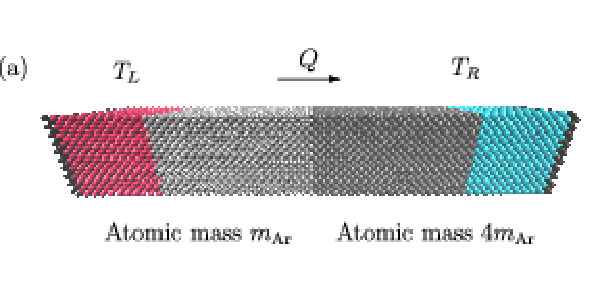
\includegraphics[width=.59\columnwidth]{inkscape/nemd_fig2a.pdf} 
  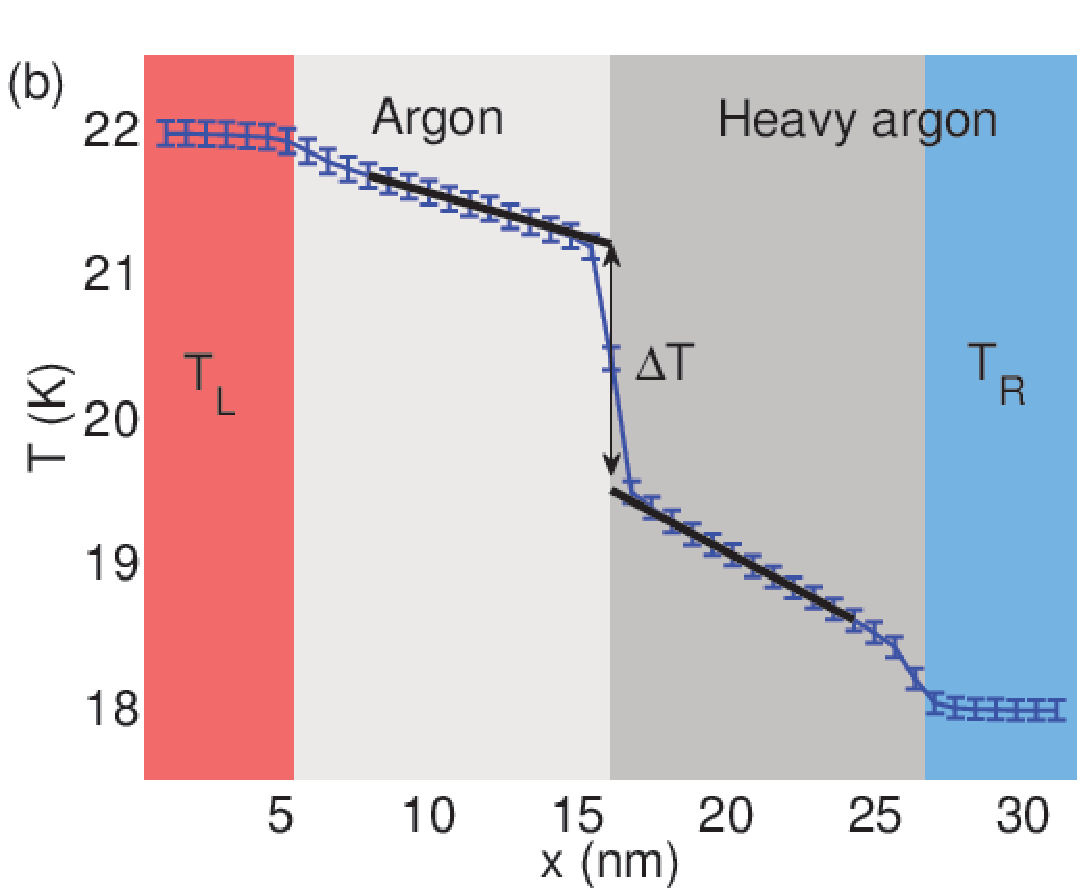
\includegraphics[width=.59\columnwidth]{inkscape/nemd_fig2b.pdf}
  \caption{(a) Simulation geometry used in \citepub{spectral} for investigating the role of anharmonic effects on vibrational energy transfer at mass-mismatched interfaces. (b) Steady-state temperature profile for a specific set of parameters. Reprinted with publisher's permission from \citepub{spectral}.}  
\label{fig:th_spectral_geom}
 \end{center}
\end{figure}

To outline the typical steps involved in a non-equilibrium simulation, consider the example setup of Fig. \ref{fig:th_spectral_geom}(a) used to investigate the anharmonic effects in interfacial heat transfer in \citepub{spectral}. In the setup of Fig. \ref{fig:th_spectral_geom}(a), the whole structure is first allowed to conform to zero-stress state by controlling atomic dynamics using a combination of a Nose-Hoover barostat and thermostat \cite{allentildesley}. Typical equilibration period consists of a few hundreds of thousands of time steps. After the initial equilibration, the size of the simulation box is fixed, and the positions of atoms located at the left- and right-most unit cells are frozen, preventing atomic sublimation at the free surfaces. Particles in the ''hot'' and ''cold'' regions, illustrated by the red and cyan coloured atoms in Fig. \ref{fig:th_spectral_geom}, are coupled to heat baths at temperatures $T_{\textrm{L}}$ and $T_{\textrm{R}}$ by including Langevin or Nos\'e-Hoover terms in their equations of motion. The system is then allowed to reach non-equilibrium steady state by integrating the equations of motion until the kinetic temperature profile shown in Fig. \ref{fig:th_spectral_geom}(b) and the heat current flowing through the system fluctuate around constant values. After this transient period, simulation is continued typically for millions of time steps, and the values of observables such as temperature jump $\Delta T$ at the interface or the heat currents are determined from the trajectories. The statistical error in the determined quantities can be estimated by using standard methods described, e.g., in Ref. \cite{allentildesley}.

LAMMPS simulation package \cite{plimpton95} is used in Publications \cp{spectral}, \cp{cnt} and \cp{twinning} for integrating the equations of motion. The simulations of Publications \cp{fpu} and \cp{fpu2} are carried out using a house-made MD code. 

\section{Limitations of molecular dynamics and Green's function models}
\label{sec:th_limits}
MD and GF methods presented in the above sections are used in this thesis to investigate phononic energy transfer. Because MD is fully classical and therefore neglects all quantum effects, the method is strictly valid only at temperatures higher than the Debye temperature $T_D$ of the material under study\footnote{Debye temperature is defined here as $T_D=\hbar \omega_{max}/k_B$, where $\omega_{max}$ is the frequency of the highest-energy phonon mode.}. Despite this limitation, MD is still widely used and considered suitable \cite{cahill14} also at temperatures lower than $T_D$ due to its ability to capture the complex atomistic dynamics of solids, liquids, and gases, inherently including also non-linear effects through the anharmonic terms in the interatomic potential. MD can therefore deliver powerful physical insight into the energy transfer processes taking place in nanosystems.

In contrast to MD, the GF method fully captures quantum statistics. Being based on the algebraic solution of the linearized Langevin equations of motion, the method also straightforwardly delivers the spectrally decomposed thermal current [Eq. \eqref{eq:th_caroli}], which is only indirectly available from MD [Eq. \eqref{eq:th_spectral_curr}]. The drawback of the GF method is that it can only account for dissipative effects in terms of a single frequency-independent relaxation time given as an input parameter. The method is therefore not suitable for calculating, e.g., the thermal conductivity of materials. In addition, the method assumes small displacements of atoms from their equilibrium positions and cannot therefore be applied to the modeling of liquids, gases, or soft solids.

In addition to MD and GF methods, energy transfer in nanoscale can also be modeled using the Boltzmann transport equation \cite{ziman}. Boltzmann equation treats phonons as point-like particles and therefore neglects wave effects such as interference. The power of the method lies, however, in its applicability to large systems and its ability to straightforwardly capture various different scattering mechanisms in terms of phonon scattering rates calculated semi-empirically or from first principles methods. Recent advances in computational methods have allowed for a numerically exact solution of the Boltzmann equation in non-equilibrium, enabling parameter-free determination of thermal conductivity \cite{broido07,ward09,lindsay13}. The applicability of the Boltzmann equation to the nanoscale structures considered in this thesis is, however, questionable due to its inability to capture interference effects, so only atomistic simulation methods are used in this thesis.


\chapter{Results and discussion}

\label{chap:results}

The main results of this thesis are grouped into three different sections according to the studied phenomena and the used methods. Sections \ref{sec:results_anharm} and \ref{sec:results_interference} summarize the results of non-equilibrium molecular dynamics (NEMD) modeling of lattice heat transfer in various geometries, focusing on anharmonic scattering and wave interference phenomena, respectively. Section \ref{sec:results_gf} highlights the Green's function (GF) approach to modeling quantum effects in phonon transport and the cavity-enhancement of electromagnetic energy transfer.

\section{Anharmonic effects in phononic thermal conduction}
\label{sec:results_anharm}

Phonon-phonon scattering arises from the anharmonic terms in the interatomic potential as discussed in Sec. \ref{sec:th_eom2}. These terms are crucial in first-principles modeling of thermal conduction at interfaces and bulk, because they boost heat transfer across interfaces \cite{lyeo06} and are responsible for the thermal resistivity of pristine bulk materials. Combining NEMD and the spectral decomposition formula \eqref{eq:th_spectral_curr} for the heat current, one can extract detailed information of the effects of these non-linear terms on thermal conduction. Subsection \ref{sec:results_interface} studies the heat current spectrum at the interface between two mass-mismatched materials at different temperatures, revealing two different heat transfer mechanisms relying on anharmonic effects. Subsection \ref{sec:results_mfps} investigates the dependence of the spectral heat current on the tube length in carbon nanotubes, allowing for determining phonon mean free paths at each vibrational frequency. 

Finally, NEMD is used in Subsection \ref{sec:results_twinning} to investigate the effects of periodic twinning on the thermal conductivity in silicon nanowires. Twinning stacking faults are common defects occurring in the vapor-liquid-solid growth of semiconductor nanowires \cite{johansson06,xiong06,davidson07,algra08}, and while their applicability in the tuning of electronic \cite{ikonic93b} and optical \cite{ikonic95} properties has already been demonstrated \cite{im14}, their effect on the thermal properties of nanowires is unknown. The results described in Subsection \ref{sec:results_twinning} suggest that periodic twinning can increase the thermoelectric figure of merit of silicon nanowires. 

\subsection{Interfacial thermal conduction}
\label{sec:results_interface}

The role of anharmonic phonon scattering in interfacial thermal conduction was investigated in \citepub{spectral} using the computational setup presented earlier in Fig. \ref{fig:th_spectral_geom}. Atoms with masses $m_{\textrm{Ar}}=28$ amu (atomic mass of argon) and $4m_{\textrm{Ar}}$ were placed to fill two half-spaces in a face-centered cubic lattice, with the atoms of the two half-spaces being separated by a plane with surface normal along the [100] direction as depicted in Fig. \ref{fig:th_spectral_geom}. The mass-mismatch induces an acoustic mismatch between the materials, creating a non-zero contact resistance for phonons. Interatomic interactions were modeled using the Lennard-Jones potential \cite{allentildesley} and the interaction parameters were chosen to correspond to solid argon \cite{allentildesley}. \change{The bath temperature difference $\Delta T=T_L-T_R$ was set to $\Delta T=T/3$ in all simulations. We carefully checked that the conductance spectra did not visibly change when $\Delta T$ was reduced, ensuring that non-linear contributions to the heat current [proportional to $(\Delta T)^2$ and higher powers of $\Delta T$] were negligible.}

\begin{figure}[tb]
 \begin{center}
  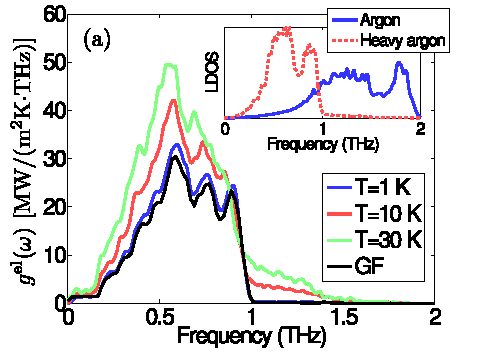
\includegraphics[width=.49\columnwidth]{pics/nemd_fig4a.pdf}
  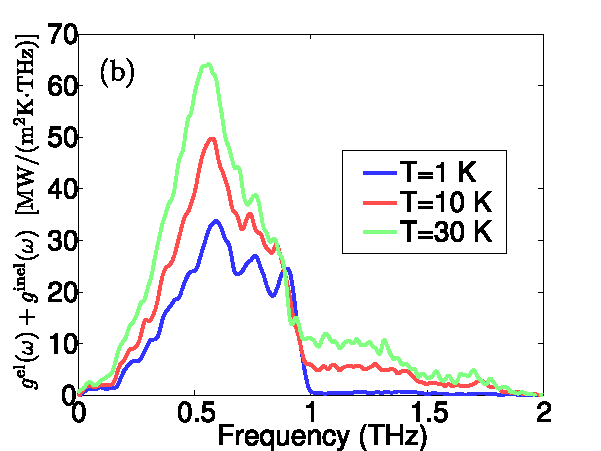
\includegraphics[width=.49\columnwidth]{pics/nemd_fig4b.pdf}
  \caption{Elastic thermal conductance $g^{\textrm{el}}(\omega)=q(\omega)/\Delta T_b$ through the acoustically mismatched interface as a function of frequency at various temperatures.  At $T=1$ K, the elastic conductance agrees with the Landauer-B\"uttiker conductance calculated using the GF method. At high temperatures, anharmonic scattering in the bulk enables energy transfer even above the cut-off frequency of the heavier solid, located at 1 THz.  Inset: Local density of vibrational states (LDOS, arbitrary units) at the interface. (b) The sum $g^{\textrm{el}}(\omega)+ g^{\textrm{inel}}(\omega)$ of elastic and inelastic spectral conductance as a function of frequency. The inelastic conductance describes energy transfer by phonon-phonon interactions across the interface and is defined in detail in \citepub{spectral}. At high temperatures, the anharmonic energy transfer processes strongly enhance interfacial heat transfer at $f\approx 0.5$ THz and above the cut-off of the heavier material (1 THz). Figure reprinted with publisher's permission from \citepub{spectral}.} 
 \label{fig:nemd_fig2}
 \end{center}
\end{figure}

Figure \ref{fig:nemd_fig2}(a) shows the elastic spectral conductance $g^{\textrm{el}}(\omega)=q(\omega)/\Delta T_b$, defined as the first-order contribution to the spectral current $q(\omega)$ [Eq. \eqref{eq:th_spectral_curr}] calculated at the interface divided by the temperature jump $\Delta T_b$. Conductance $g^{\textrm{el}}(\omega)$ is referred to as elastic, because it is calculated from the coupling of vibrations at the same frequency $\omega$ at different sides of the interface. The first-order conductance accounts, however, also for inelastic effects through the non-linear phonon dynamics calculated from NEMD with all orders of interactions. 

As seen in Fig. \ref{fig:nemd_fig2}(a), modes with frequencies above 1 THz cannot carry energy across the interface at low temperature ($T=1$ K), because there are no propagating modes in the heavier material above 1 THz. This absence of modes is evident in the interfacial density of states depicted in the inset of Fig. \ref{fig:nemd_fig2}(a), where only a small tail induced by the evanescent modes is visible above 1 THz in the heavy material. At higher temperatures ($T=10$ K and $T=30$ K), the onset of anharmonic effects can be seen to enable evanescent energy transfer across the interface. Most notably, anharmonic effects enable energy transfer even above the cut-off frequency of the heavier material. These high-frequency modes are evanescent in the heavier material, but they can dissipate their heat to lower-frequency modes in the immediate vicinity of the interface through anharmonic interactions. Our results are the first to explicitly demonstrate energy transfer across interfaces by such evanescent wave dissipation.

To further probe the role of anharmonic scattering in interfacial energy transfer, we determined also the first-order anharmonic contribution to the spectral heat current at the interface. The expression for this first-order anharmonic conductance $g^{\textrm{inel}}(\omega)$, which is referred to as inelastic due to its natural interpretation as describing three-phonon energy transfer processes, was derived from the second-order contribution to spectral heat current as detailed in \citepub{spectral}. The sum of elastic and inelastic contributions to the conductance is shown in Fig. \ref{fig:nemd_fig2}(b). Comparison to Fig. \ref{fig:nemd_fig2}(a) shows that the three-phonon energy transfer processes enhance energy transfer across the whole frequency range between zero and 2 THz, both below and above the cut-off frequency of the heavy argon. As discussed in detail in \citepub{spectral}, these inelastic energy transfer processes are dominated by frequency-doubling and frequency-halving anharmonic processes at the interface, thereby supporting the phenomenological higher harmonic inelastic model suggested earlier by Hopkins \cite{hopkins09_jap}. Because of the high computational burden required for determining the contributions of higher-order anharmonic processes to the conductance and the complexity of analyzing such terms, the analysis of \citepub{spectral} was limited to first-order anharmonic processes.

Our results are the first to quantify the contributions of anharmonic processes to interfacial energy transfer from atomistic simulations and have facilitated the physical interpretation of experimental results for the interfacial conductance between metals and diamond \cite{hohensee15}. 

\subsection{Mean free paths in carbon nanotubes}

\label{sec:results_mfps}

\begin{figure}[tb]
 \begin{center}
  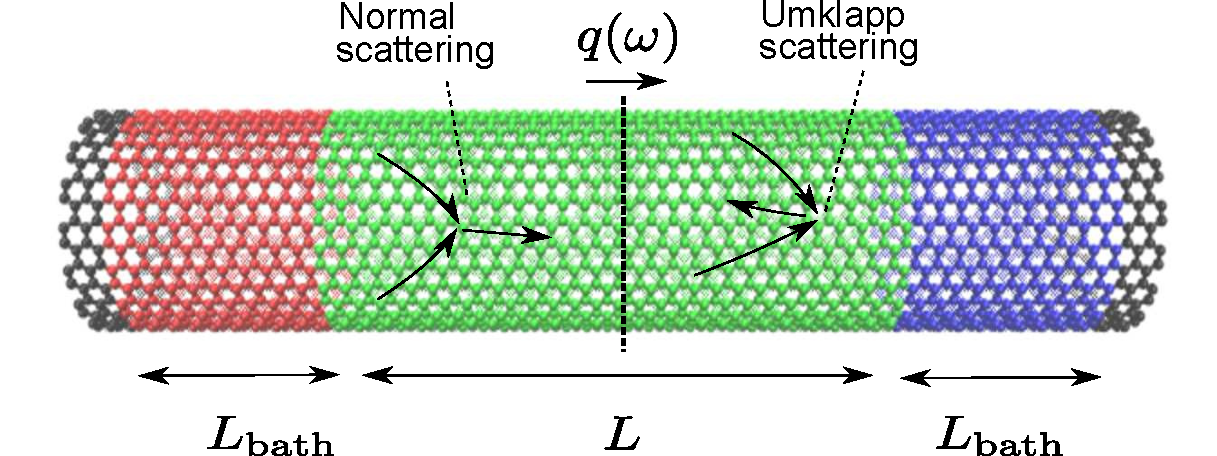
\includegraphics[width=.89\columnwidth]{pics/cnt_fig1-crop.pdf} 
  \caption{Schematic illustration of the NEMD setup used for determining the length-dependent thermal conductivity and phonon mean free paths in carbon nanotubes. When traversing the tube, phonons undergo both normal and Umklapp processes giving rise to length-dependent spectral heat current $q(\omega)$ in the tube. From the $L$-dependence of $q(\omega)$, one can determine the mean free paths at each frequency as described in \citepub{cnt}. Figure reprinted with publisher's permission from \citepub{cnt}.}  
\label{fig:cnt_fig1}
 \end{center}
\end{figure}

Carbon nanotubes have a very high thermal conductivity in the range 500-5000 W/mK \cite{marconnet13}, and their thermal conductivity has been found to increase as a function of tube length in tubes as long as 5 $\upmu$m \cite{chang08} and, very recently, even in tubes as long as 1 mm \cite{chang_personal}. Theoretical understanding of the limits of ballistic heat transfer in carbon nanotubes is of crucial importance for their applications in, e.g., thermal management \cite{biercuk02,huang05}. The goal of \citepub{cnt} was to shed insight to the ballistic limits of thermal conductivity in pristine nanotubes by determining the spectral contributions to the thermal current \eqref{eq:th_spectral_curr} in tubes of different lengths $L$ from atomistic simulations. \change{From the length-dependent current $q(\omega;L)$, we first determined the generalized phonon transmission function}
\begin{equation}
 \ca{T}(\omega) = \frac{q(\omega;L)}{k_B \Delta T}, \label{eq:Tomega_L}
\end{equation}
\change{which is essentially the phonon transmission probability through a tube of length $L$ summed over all propagating modes at angular frequency $\omega$. We then determined the mean free paths $\Lambda(\omega)$ by fitting the length-dependent transmission \eqref{eq:Tomega_L} to the equation }\cite{datta,wang06_apl,savic08_prl}
\begin{equation}
 \ca{T}(\omega) = \frac{M(\omega)}{1+L/\Lambda(\omega)}.
\end{equation}
\change{Here $M(\omega)$ is the number of propagating modes in the nanotube in the ballistic limit.}

 %This length-dependence was used to calculate frequency-dependent phonon mean free paths. % The simulated tube lengths exceed 

Figure \ref{fig:cnt_fig1} shows the schematic illustration of the NEMD setup used for carbon nanotubes of (10,10) chirality. Regions of length $L_{\textrm{bath}}=10$ nm were coupled to Langevin thermostats at temperatures $T+\Delta T/2$ and $T-\Delta T/2$ to drive heat current through the tube, and the frequency-dependent phonon mean free paths were determined from the decrease of the non-equilibrium spectral heat current \eqref{eq:th_spectral_curr} at different frequencies as a function of tube length $L$. The decrease in spectral current arises from anharmonic interactions, which are fully accounted for by the non-linear terms of the optimized Tersoff potential used for modeling carbon-carbon interactions \cite{tersoff88a,lindsay10}. In contrast to equilibrium mean free paths, which characterize the equilibrium scattering lengths arising from the combined effect of normal and Umklapp processes \cite{mcgaughey04}, the mean free paths determined from NEMD \textit{directly reflect the resistance to the heat flow} (expected to be dominated by Umklapp processes). % For a detailed account of the method, we refer to \citepub{cnt}.


\begin{figure}[tb]
 \begin{center}
  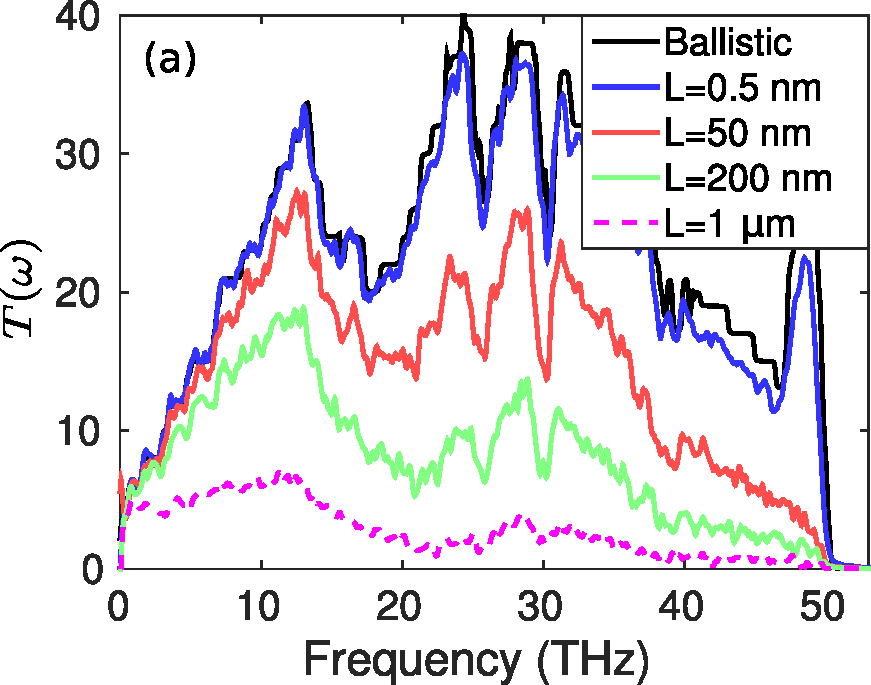
\includegraphics[width=.49\columnwidth]{pics/cnt_fig2_mod.pdf} 
  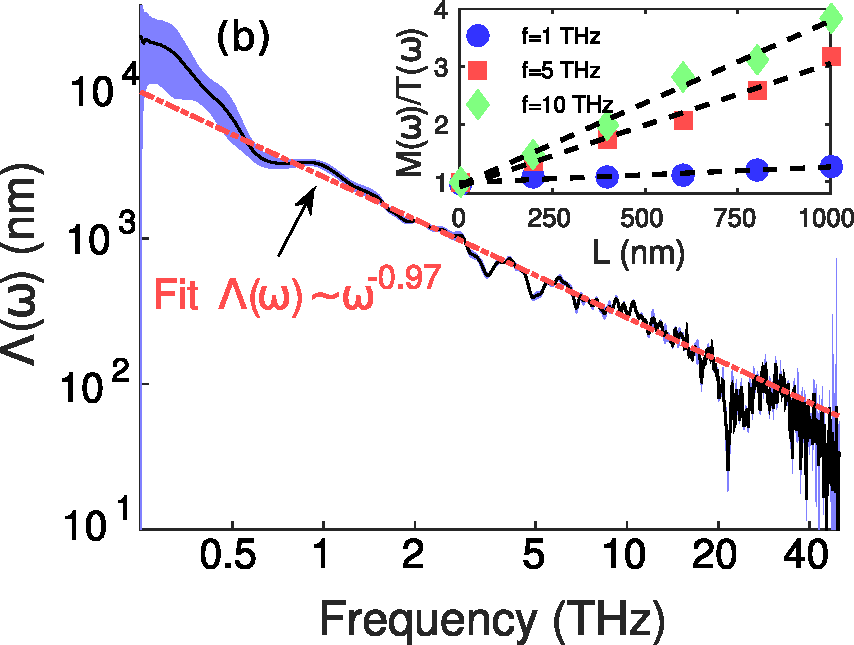
\includegraphics[width=.49\columnwidth]{pics/cnt_fig4_new.pdf} 
  \caption{(a) Generalized phonon transmission function $\ca{T}(\omega)=q(\omega)/(k_B\Delta T)$ for different tube lengths at $T=300$ K. Increasing the tube length reduces the transmission due to anharmonic scattering. For $L=0.5$ nm, phonon transmission is nearly equal to the ballistic value determined by counting the number of propagating modes in the nanotube. (b) Log-log plot of the mean free path $\Lambda(\omega)$ at $T=300$ K, determined from the slope of the inverse transmission function as a function of tube length $L$ as illustrated by the dashed lines in the inset. The shaded regions in the main figure correspond to the 92.5\% confidence interval for the slope. Below 0.25 THz, the confidence interval is large due to numerical uncertainties, preventing the determination of mean free paths at the lowest frequencies. Figure reprinted with publisher's permission from \citepub{cnt}.}  
\label{fig:cnt_fig2}
 \end{center}
\end{figure}

Figure \ref{fig:cnt_fig2}(a) shows the generalized phonon transmission function $\ca{T}(\omega)$ for different tube lengths $L$. For $L=0.5$ nm, the transmission probability of each mode is unity and the generalized phonon transmission is nearly equal to the number of propagating phonon modes (black solid line). As the tube length increases, anharmonic scattering reduces the transmission. This reduction is strongest at high frequencies, suggesting that the mean free path decreases as a function of frequency, which is reasonable considering the larger phase-space available for phonon-phonon scattering at high frequencies \cite{ziman}.

Phonon mean free paths are plotted as a function of frequency in Fig. \ref{fig:cnt_fig2}. The mean free paths are calculated using the fitting procedure depicted in the inset of Fig. \ref{fig:cnt_fig2} and described in detail in \citepub{cnt}. The results show that the mean free paths obey a power-law $\Lambda(\omega)\propto \omega^{-\alpha}$ as a function of frequency in a large frequency interval, with a different exponent $\alpha\approx 0.97$ than the value $\alpha=2$ used earlier \cite{wang06_apl} to phenomenologically describe the ballistic-diffusive transition in carbon nanotubes. \change{This disagreement is not surprising, because the value $\alpha=2$ has been derived \cite{ziman} for three-dimensional bulk systems and is therefore expected to break down in quasi-one-dimensional nanotubes. The exact value of the exponent $\alpha$ is also sensitive to the detailed geometry of the system, as suggested by recent results for one-dimensional anharmonic chains, for which the value $\alpha\approx 1.67$ has been found \cite{saaskilahti15b}}. At low frequencies, the mean free paths shown in Fig. \ref{fig:cnt_fig2} exceed 10 $\upmu$m, in agreement with the strong length-dependence of the experimentally measured thermal conductivity in nanotubes as long as $5$ $\upmu$m \cite{chang08}. 

The numerical results for the phonon mean free paths show that thermal conduction in carbon nanotubes is partially ballistic at least up to micrometer scale. At very low frequencies ($f\lesssim 0.1$ THz), the mean free paths might extend even up to millimeter scale. This conclusion contradicts earlier simulation results \cite{thomas10b} showing the convergence of thermal conductivity in 1 $\upmu$m long nanotubes. The disagreement most likely originates from the different interatomic potential used in the simulations: the REBO potential \cite{brenner02} employed in Ref. \cite{thomas10b} is known to underestimate the thermal conductivity of carbon nanomaterials \cite{salaway14}. 

% Analysis of the spectral thermal conductivity $\kappa(\omega)=Lq(\omega)/\Delta T$ in \citepub{cnt} reveals that modes with frequencies 

% \textbf{DISCUSS THE LIMITS OF BALLISTIC CONDUCTION}

\subsection{Thermal conductivity reduction in twinning nanowires}

\label{sec:results_twinning}

Efficient thermoelectric conversion generally requires materials with low thermal conductivity and high electronic conductivity \cite{majumdar04}. Nanostructuring is known to be an effective way to reduce the thermal conductivity by increasing phonon scattering \cite{vineis10,shakouri11}. In silicon nanowires, for example, phonon scattering from the rough nanowire surfaces and the reduction in the phonon group velocity due to spatial confinement \cite{balandin98} reduce the thermal conductivity by two orders of magnitude compared to the bulk value \cite{hochbaum08,boukai08}, thereby increasing the thermoelectric figure of merit \cite{chen} close to unity. To investigate possibilities to increase the thermoelectric efficiency of Si nanowires even further, \citepub{twinning} studied the effect of periodic twinning stacking faults \cite{algra08,caroff09} on the thermal properties of Si nanowires.


\begin{figure}[tb]
 \begin{center}
  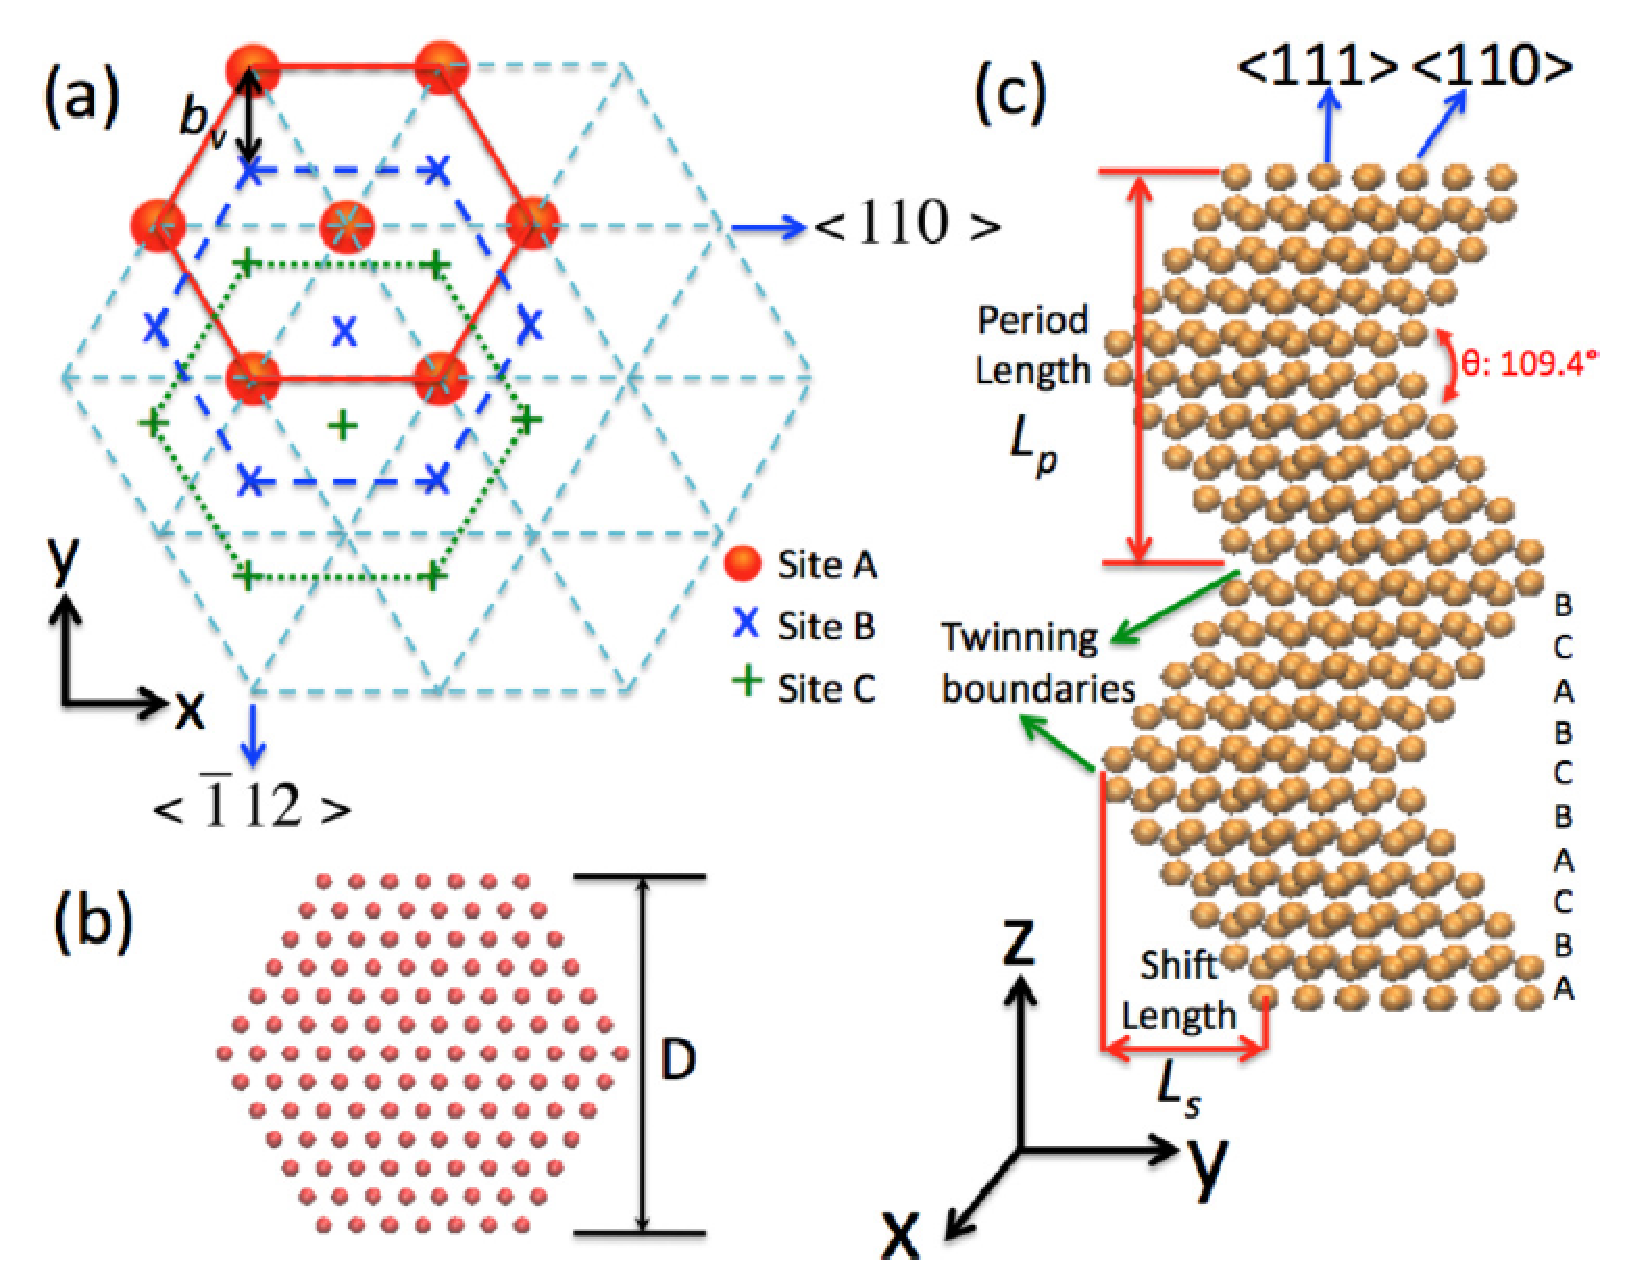
\includegraphics[width=.89\columnwidth]{pics/twinning_fig1.pdf} 
  \caption{(a) Schematic illustration of stacking in the close-packed silicon lattice. Stacking fault occurs when the stacking sequence ABCABC is locally changed to ABCBAC. (b) Cross-section of the nanowire. (c) Silicon nanowire with twinning boundaries. The period length is denoted by $L_p$ and the ''shift length'' $L_s$ is related to $L_p$ by $L_s=(L_p/2)\cot(\theta/2)$, where $\theta=109.4^{\circ}$. The figure also illustrates the perturbation of the ABCABC... stacking sequence at the twinning boundaries. Figure reprinted with publisher's permission from \citepub{twinning}.}  
\label{fig:twinning_fig1}
 \end{center}
\end{figure}

Twinning stacking faults \cite{cahn54} are common defects appearing in the vapor-liquid-solid growth of nanowires made of group IV and group III-V nanowires \cite{johansson06,xiong06,davidson07,algra08}. At a twinning interface, the crystallographic orientation of the nanowire changes without leaving any dangling bonds \cite{korgel06}. In the Si nanowire illustrated in Fig. \ref{fig:twinning_fig1}, the twinning interface essentially joins two nanowires with different stacking orders as depicted in Figs. \ref{fig:twinning_fig1}(a) and (c), giving rise to periodically repeating kinks in the nanowire. Such periodic kinks perturb phonon propagation in the nanowire and are expected to therefore reduce the thermal conductivity. Periodically twinned Si nanowires have been recently grown experimentally \cite{ruffino15}.

The computational NEMD setup of \citepub{twinning} was similar as for the carbon nanotubes considered in \citepub{cnt}, with the exception that Langevin heat baths were replaced by deterministic Nos\'e-Hoover thermostats \cite{nose84,hoover85} and interatomic potential was replaced by the Stillinger-Weber potential \cite{stillinger85} modeling silicon-silicon interactions. The cross-section of the nanowires was chosen to be hexagonal with diameter $D$ as shown in Fig. \ref{fig:twinning_fig1}(b). The twinning period is denoted by $L_p$, corresponding to the ''shift length'' $L_s=(L_p/2)\cot(\theta/2)$, where $\theta=109.4^{\circ}$ is the kink angle as shown in Fig. \ref{fig:twinning_fig1}(c). 


\begin{figure}[tb]
 \begin{center}
   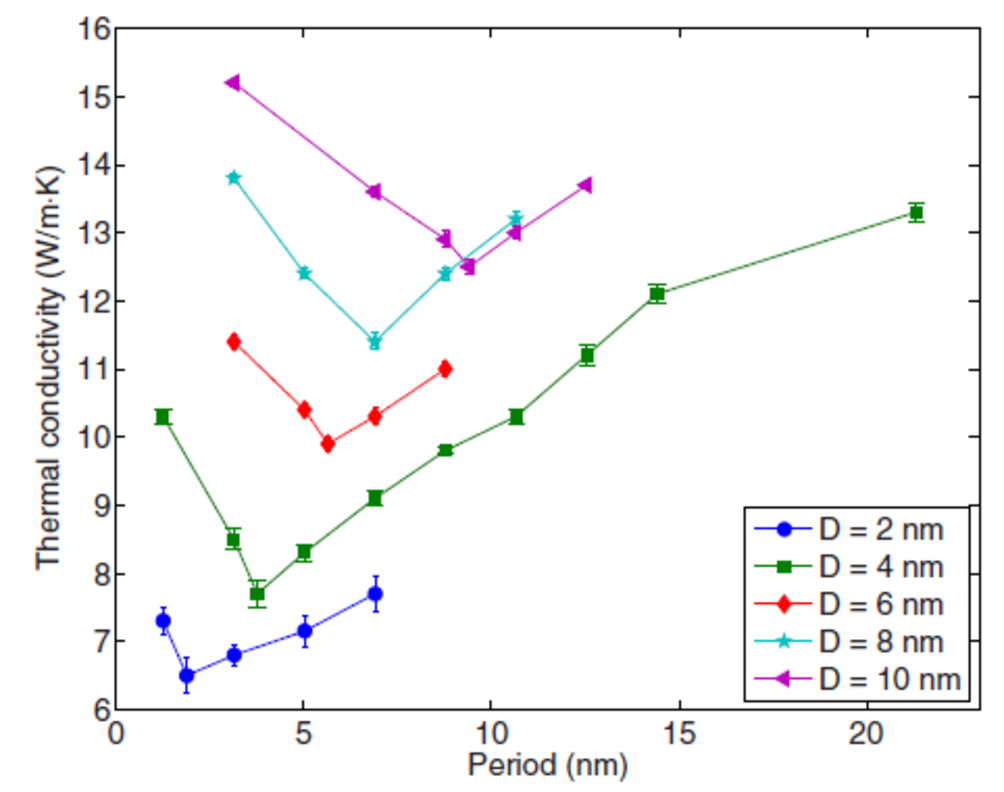
\includegraphics[width=.89\columnwidth]{pics/twinning_fig2a_mod.pdf} 
  \caption{Thermal conductivity of silicon twinning nanowires at $T=300$ K as a function of period length $L_p$ for different diameters $D$. For each diameter $D$, there is a corresponding minimum in the thermal conductivity as a function of period length. The minimum arises from the competition between geometric and anharmonic effects as shown in \citepub{twinning}. Figure reprinted with publisher's permission from \citepub{twinning}.}  
\label{fig:twinning_fig2}
 \end{center}
\end{figure}

Thermal conductivity of the twinning nanowires as a function of period $L_p$ are shown in Fig. \ref{fig:twinning_fig2} for different diameters $D$. For each diameter, there is a corresponding period length with a minimum in the thermal conductivity. Lowest conductivity was found for the period length $L_p\approx 0.95D$, corresponding to the shift length $L_s=D/3$. The detailed mechanisms behind the minimum thermal conductivity were analyzed in detail in \citepub{twinning}, with the conclusion that it \change{essentially} arises from the \change{interplay of} geometric and anharmonic scattering. \change{When the period is very small, the twinning as (small) surface roughness and resistance to heat flow is dominated by anharmonic effects. When the period gets longer, phonons are forced to change propagation direction at the kinks, increasing the geometric scattering and reducing the conductivity. When the period is very long, however, scattering at kinks becomes infrequent and the resistance is again determined by anharmonic scattering. Therefore, a minimum in the conductivity as a function of period is expected.}

The results of \citepub{twinning} show that periodical twinning can reduce the thermal conductivity of Si nanowires by 65\% compared to the straight wire.  Because the reduction of electronic conductivity is expected to be smaller due to the smaller wavelength of electrons, twinning could be used to enhance the thermoelectric performance of Si nanowires. To reduce thermal conductivity even further, periodically twinned Si nanowires could be partially amorphized \cite{donadio09} or coated with germanium \cite{hu11}. 

\section{Interference effects in phononic thermal conduction across point contacts}
\label{sec:results_interference}

For applications in thermionic \cite{zeng06}\cite{westover08} and thermophotonic \cite{oksanen08} cooling as well as thermophotovoltaic generation \cite{dimatteo01}, good thermal insulation between two bulk materials separated by a nanoscale gap is required. While a pure vacuum gap would be optimal in preventing the propagation of phonons through the gap, practical applications require structural support in the form of nanoscale point contacts bridging the gap. Such point contacts conduct heat and can therefore disturb thermal insulation. Thermal conduction properties of point contacts between bulk materials have therefore become of both theoretical \cite{saha07} and experimental \cite{bartsch12} interest in recent years.

Because the feature sizes of nanoscale point contacts can be comparable to thermal phonon wavelengths \change{and coherence lengths}, interference effects can play an important role in thermal conduction across the contact. Identification of interference effects in point contacts could possibly be exploited for thermal conductivity engineering in the same way as, e.g., in phononic crystals \cite{maldovan13}.

\begin{figure}
\begin{center}
 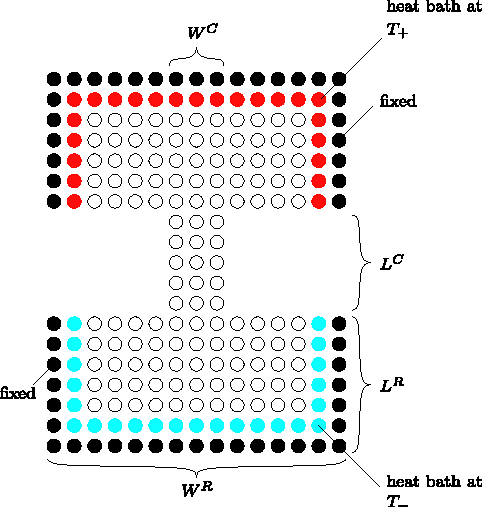
\includegraphics[width=.60\columnwidth]{pics/fpu_fig1_mod.pdf}
 \caption{Schematic illustration of the simulation setup for a point contact in a two-dimensional square lattice. Figure reprinted with publisher's permission from \citepub{fpu}.}
\label{fig:fpu_fig1}
\end{center}
\end{figure}

To investigate thermal conduction and interference effects in point contacts, we performed NEMD simulations using the simulation setup schematically illustrated in Fig. \ref{fig:fpu_fig1}. Atoms were placed in a square lattice, with the particles at the boundaries of the bulk parts at the top or bottom being either fixed (black circles) or coupled to Langevin baths at temperature $T_+$ (red circles) or $T_-$ (cyan circles). In \citepub{fpu}, the large bulk parts were connected by a rectangular point contact that is $L^C$ atoms long and $W^C$ atoms wide. Triangular and discoidal shaped point contacts were considered in \citepub{fpu2}. 

Lattice dynamics in the setup of Fig. \ref{fig:fpu_fig1} was modeled by coupling all nearest-neighbor atom pairs by anharmonic springs (not shown), whose potential energies include both quadratic and quartic terms. This potential was used by Fermi, Pasta and Ulam to investigate thermalization in one-dimensional systems \cite{fermi55} and is therefore called Fermi-Pasta-Ulam potential. The simple form of the Fermi-Pasta-Ulam potential allows for scaling the anharmonicity by a corresponding scaling in temperature, so one can present results for a single value of anharmonicity parameter without loss of generality. This scaling and other simulation details are presented in \citepub{fpu}.


\begin{figure}
\begin{center}
 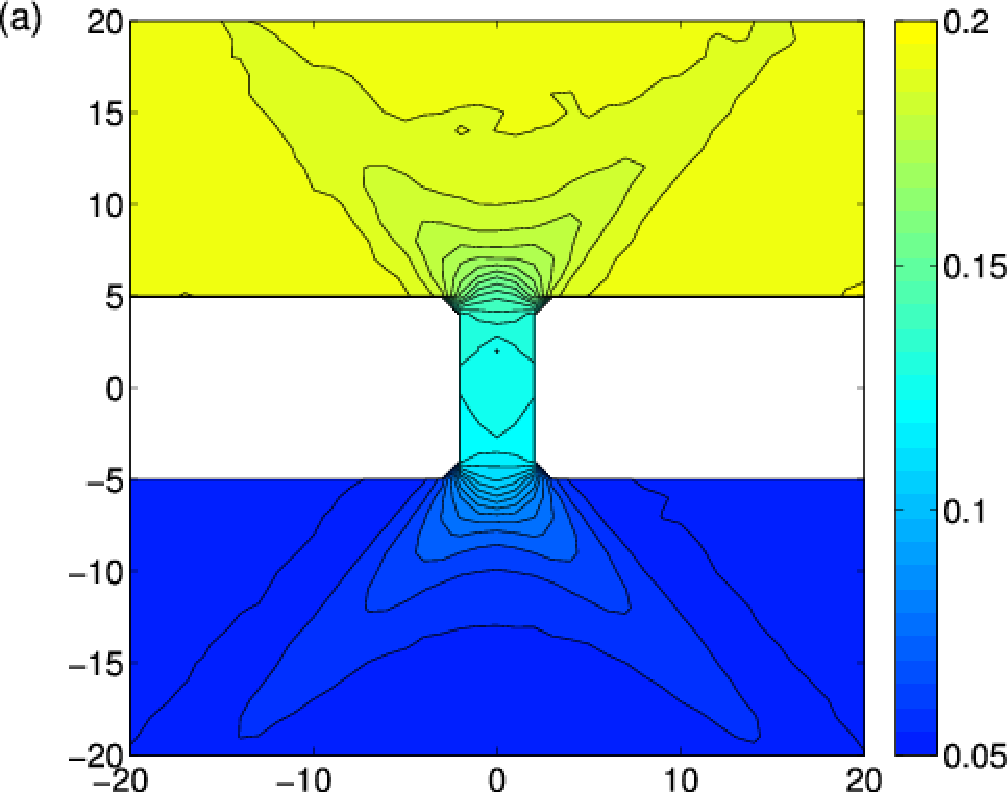
\includegraphics[width=.49\columnwidth]{pics/fpu_fig2a.pdf}
  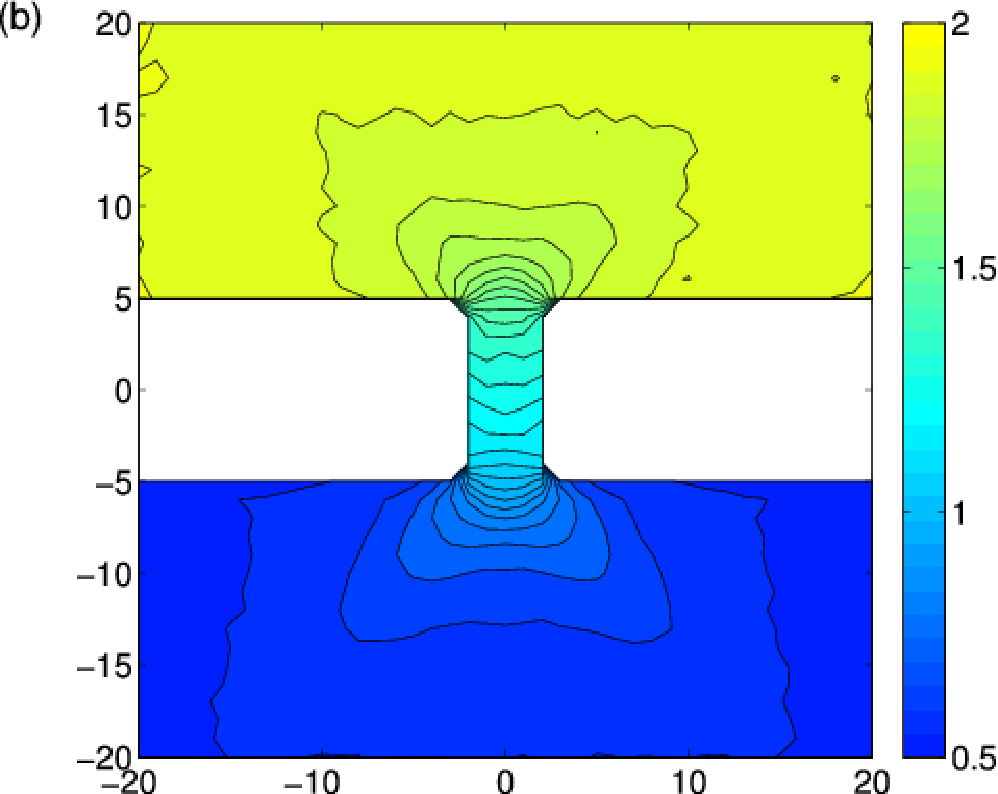
\includegraphics[width=.49\columnwidth]{pics/fpu_fig2b.pdf}
 \caption{Kinetic temperature profile at (a) low temperature ($T_+=0.20$, $T_-=0.05$) and (b) high temperature ($T_+=2.0$, $T_-=0.5$). The bulk size is $W^R=161$, $L^R=80$ and the contact size $W^C=5$, $L^C=9$ (see Fig. \ref{fig:fpu_fig1}). The labels on the horizontal and vertical axes mark the atom indices. Figure reprinted with publisher's permission from \citepub{fpu}.}
\label{fig:fpu_fig2}
\end{center}
\end{figure}

Figure \ref{fig:fpu_fig2} shows the kinetic temperature $T_i^{\textrm{kin}}=\langle mv_i^2 \rangle/k_B$ at each atomic site $i$ in a contour plot at (a) low temperature and (b) high temperature for a rectangular contact of length $L^C=9$ and width $W^C=5$. \change{Temperatures are given in the units of $T_0=m^2\omega_0^4/\beta$, where $\omega_0$ is the resonance frequency of the springs connecting the atoms and $\beta$ is the potential anharmonicity parameter defined in} \citepub{fpu}. At low temperature, lattice waves can propagate without losses and, therefore, temperature is nearly constant in the contact. Most notably, the lossless propagation can be seen to induce wavelike-features in the kinetic temperature profile in the bulk parts, with directional features along the $\langle 11 \rangle$ crystal directions. Such features contradict Fourier's law predicting a highly symmetric temperature profile with no directional features (not shown). When temperature is increased [Fig. \ref{fig:fpu_fig2}(b)], the directional features vanish and temperature profile becomes more similar to Fourier's law's prediction. Temperature profile also develops a non-zero gradient inside the contact due to the smaller thermal conductivity.


\begin{figure}
\begin{center}
 %\includegraphics[width=8.6cm]{../scbaths_paper_re_resubmission/pic1.ps}
 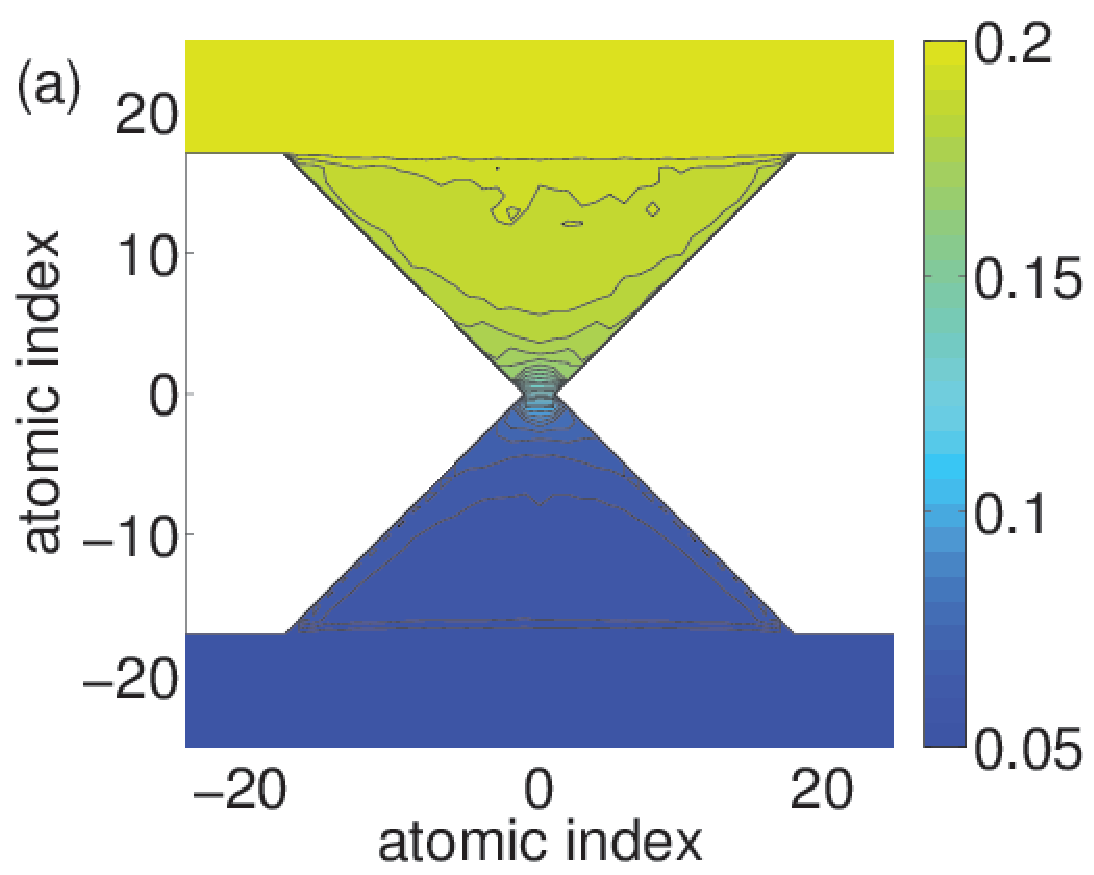
\includegraphics[width=.49\columnwidth]{pics/aip_fig5a.pdf}
 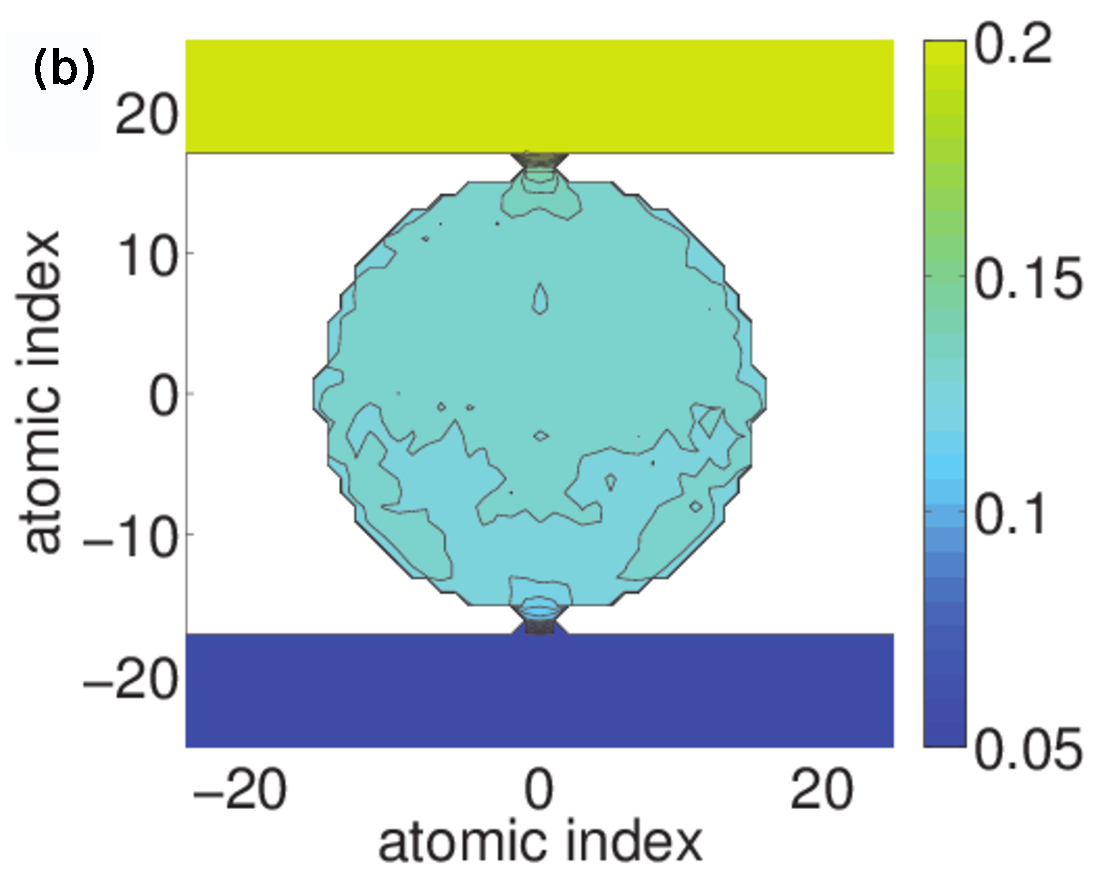
\includegraphics[width=.49\columnwidth]{pics/aip_fig6a_mod.pdf}
 %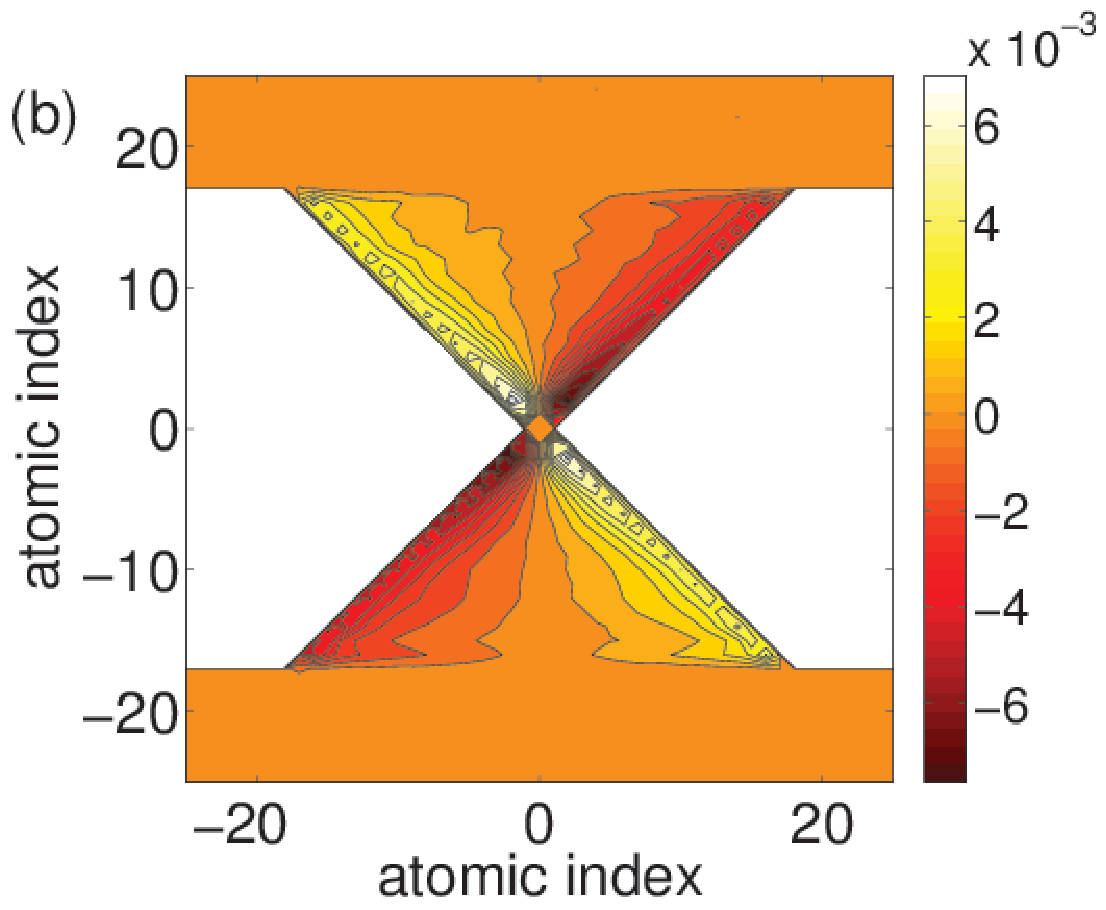
\includegraphics[width=.49\columnwidth]{pics/aip_fig5b.pdf}
 \caption{Kinetic temperature profile in (a) triangular and (b) discoidal contacts at low temperature. Figure reprinted with publisher's permission from \citepub{fpu2}.}
\label{fig:aip_figs56}
\end{center}
\end{figure}

To investigate the effects of the contact geometry on interference effects at low temperatures, calculations were performed also for hour-glass shaped and discoidal contacts. \change{Such variations in the geometry are interesting, because the point contact could be formed, e.g., by nanoparticles deposited in the vacuum gap between the materials.} Kinetic temperature profiles for the hour-glass shaped and discoidal geometries are shown in Fig. \ref{fig:aip_figs56}. For small contact areas in the triangular and discoidal contacts, temperature profiles in the bulk parts are essentially constant due to the small thermal contact between the upper and lower parts of the structure. In the triangular point contact, temperature changes nearly linearly as the contact becomes narrower. Spatial analysis of the local heat current presented in \citepub{fpu2} reveals that heat flows mainly along the edges of the triangles. In the discoidal geometry of Fig. \ref{fig:aip_figs56}(b), which could represent a nanoparticle sandwiched between two materials, temperature profile is again nearly flat inside the center region, with only small spatial variations in temperature. However, local heat currents inside the center region, shown in \citepub{fpu2}, are strongly direction-dependent, with similar enhancement in $\langle 11\rangle$ direction as in the temperature profile of Fig. \ref{fig:fpu_fig2}(a).

The results show that in the ballistic low-temperature limit, local temperature and heat current profiles can exhibit wavelike-features \change{arising from mode interference and (partially) ballistic conduction}. \change{In future, it would be useful to analyze the mean free paths and transmission probabilities of individual modes to quantitatively understand the origin of directional patterns in different geometries}. Accounting for such directional patterns could enable more efficient engineering of thermal conductivity in nanostructures. It is, however, well known that the effect of quantum statistics neglected by classical MD can be significant at low temperatures. To include quantum statistics, we turn to the quantum-mechanical GF method based on the linearized Langevin equations of motion presented in Sec. \ref{sec:th_eom}

%The results show that in the ballistic low-temperature limit, local temperature and heat current profiles can exhibit wavelike-features with interference patterns. Accounting for such directional patterns could enable more efficient engineering of thermal conductivity in nanostructures. It is, however, well known that the effect of quantum statistics neglected by classical MD can be significant at low temperatures. To include quantum statistics, we turn to the quantum-mechanical GF method based on the linearized Langevin equations of motion presented in Sec. \ref{sec:th_eom}.

\section{Langevin modeling of phononic and photonic energy transfer}
\label{sec:results_gf}

As discussed in Sec. \ref{sec:th_eom}, solving the linearized Langevin equations \eqref{eq:th_eom1}, \eqref{eq:th_eom2}, and \eqref{eq:th_eom3} in terms of the GF allows for heat transfer modeling that accounts for wave interference, quantum statistics, and even dissipative losses in terms of a frequency-independent relaxation rate. In this thesis, GF method is applied to investigate (i) quantum thermal transport through point contacts in Subsection \ref{sec:results_schb} and (ii) cavity-en\-hance\-ment of electromagnetic energy transfer rates between SiC nanoparticles in Subsection \ref{sec:results_cavity}. 

\subsection{Quantum effects in point contacts}
\label{sec:results_schb}

Application of the linearized Langevin equation \eqref{eq:th_eom1} for lossy phonon transport is closely related to the self-consistent heat bath model \cite{bolsterli70}, discussed in detail in this Subsection. Whereas earlier works have applied the model to simple one-dimensional systems (see, e.g., Refs. \cite{bolsterli70,visscher75,dhar03,dhar06,segal09,bandyopadhyay11}) with a finite number of atoms, \citepub{gf} extended the model to more complex geometries with an infinite number of atoms.  

The setup of \citepub{gf} is schematically illustrated in Fig. \ref{fig:schb_setup}. The setup consists of a center region with a finite number of atoms and left and right leads with possibly an infinite number of atoms. All atoms are coupled to local Langevin baths mimicking all interaction events driving the system towards local thermal equilibrium \cite{bolsterli70}. In the center region of Fig. \ref{fig:schb_setup}(a), a point contact acts as a scattering center for phonons coming in from the left and right leads. In the vicinity of the contact, bath temperatures are unknown. Following the self-consistent heat bath model \cite{bolsterli70}, these temperatures are determined self-consistently from the requirement that the heat current to each bath vanishes. The requirement of zero heat current to local baths ensures that the heat current flowing in the system is conserved at each atom site, a natural requirement in the steady-state in the absence of coupling to other carriers such as electrons.

Away from the scattering region, the baths are set to prescribed temperatures $T_L$ and $T_R$. Whereas earlier works \cite{dhar06} have modeled lattice dynamics in the leads as completely lossless, which induces an acoustic mismatch between the lossless leads and the lossy center region, the setup of Fig. \ref{fig:schb_setup} eliminates this mismatch by including losses for the leads as well.  

\begin{figure}
\begin{center}
 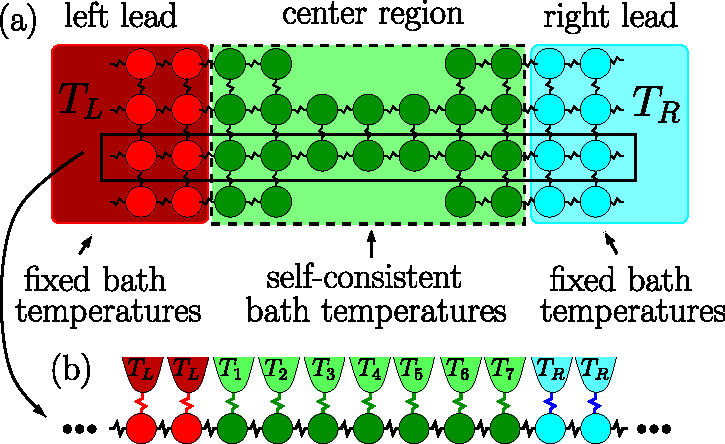
\includegraphics[width=.99\columnwidth]{inkscape/gf_fig1.pdf}
 \caption{A schematic illustration of the self-consistent heat bath model for a constriction in a two-dimensional rectangular lattice. The system consists of the left lead, the center region, and the right lead. All atoms are coupled to Langevin heat baths, shown explicitly for one cross section in (b). Whereas the temperatures of the Langevin baths have prescribed values $T_L$ and $T_R$ in the left and right lead, the bath temperatures are determined self-consistently in the center region from the requirement that the thermal current to each bath is zero \cite{bolsterli70}. Reprinted from \citepub{gf} with publisher's permission.}
\label{fig:schb_setup}
\end{center}
\end{figure} 

The calculation of heat currents starts from the Langevin equation of motion \eqref{eq:th_eom1} for each atom $i$ with interatomic force constants $\bb{K}_{ij}$ determined by the interatomic potential energy function. The relaxation rate $\gamma$ is chosen to correspond to known phonon life-times. It is shown in \citepub{gf} that solving the equations of motion for the leads and substituting to the equations for the center region allows for replacing the leads by \textit{single} Langevin heat baths at temperatures $T_L$ and $T_R$, which reduces the number of degrees of freedom to those in the center region. The microscopic details of acoustically matched lattice dynamics in the leads are fully captured by the lead self-energy functions $\Sigma^L(\omega)$ and $\Sigma^R(\omega)$. Microscopic definitions of the self-energy function in terms of the lead GF and the fluctuation-dissipation theorem for the corresponding Langevin noises are presented in detail in \citepub{gf}.

By following the procedure presented in Sec. \ref{sec:th_bathcurrents}, one can calculate the heat currents flowing to baths in terms of the center region's GF $\bb{G}(\omega)$. By setting the heat current equal to zero for the local baths in the center region, one gets a non-linear system of equations for the bath temperatures. This system of equations can be solved by, e.g., using Newton-Raphson method \cite{bandyopadhyay11} or resorting to linearizing approximations \cite{segal09}. It is shown in \citepub{gf} that the requirement of vanishing heat current to the baths is equivalent to an intuitive thermal balance condition between kinetic and potential energies. Similar thermal balance condition was recently reported for local photon number in fluctuational electrodynamics \cite{partanen14}. 

\begin{figure}
 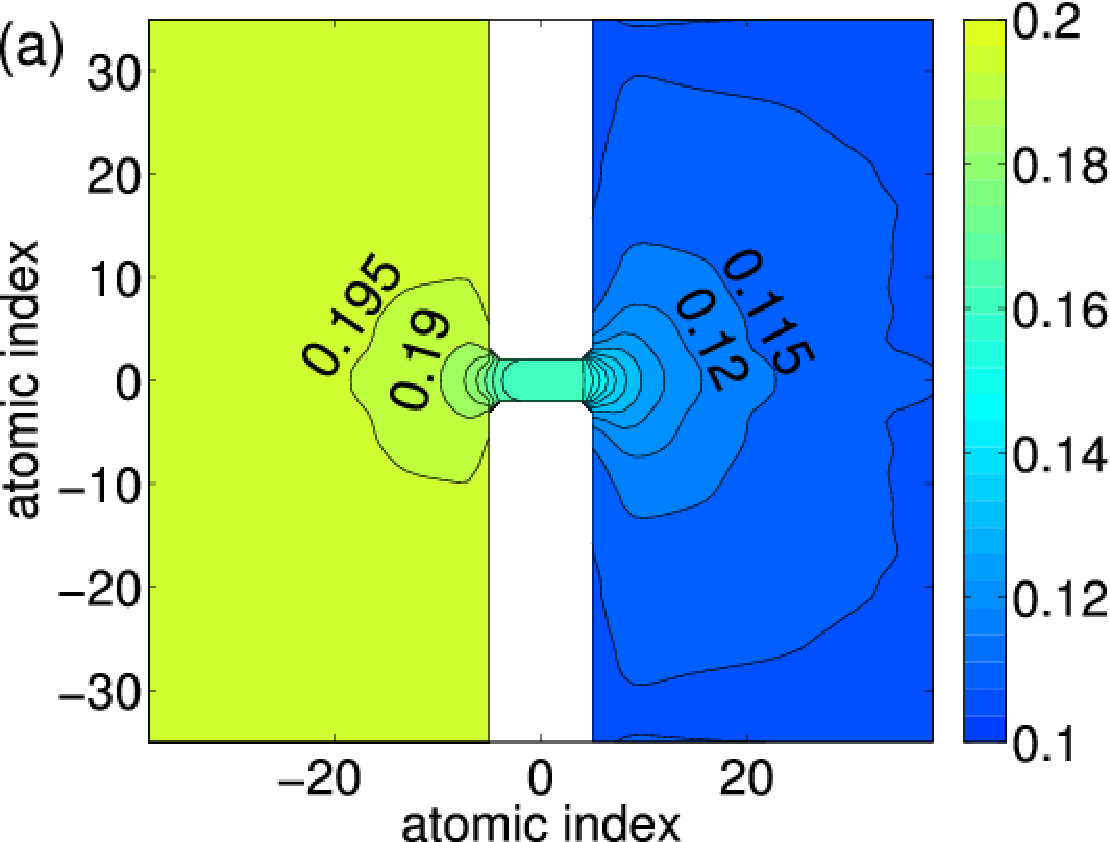
\includegraphics[width=.49\columnwidth]{pics/gf_fig7a.pdf}
 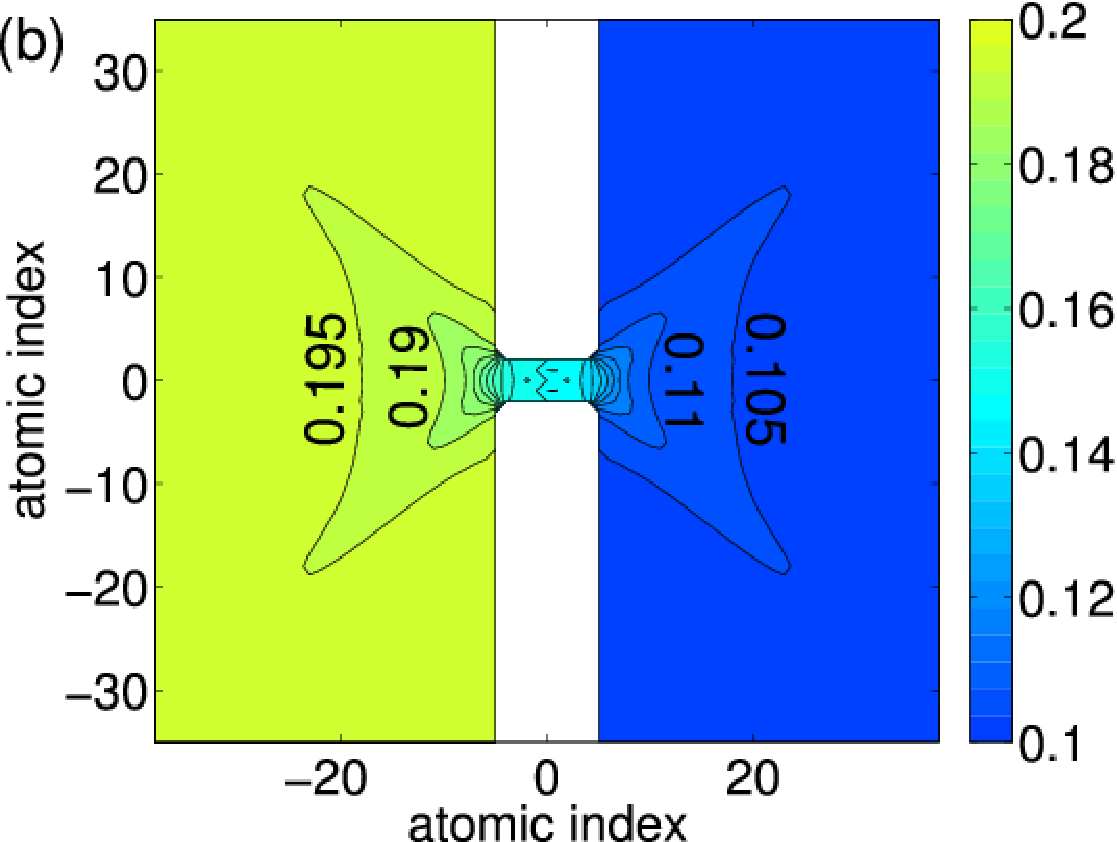
\includegraphics[width=.49\columnwidth]{pics/gf_fig7b.pdf}
 \caption{Self-consistent local bath temperature profiles in a rectangular contact connecting two square lattices. Lead temperatures are $T_L=0.2$ and $T_R=0.1$. Figures show temperature profiles for (a) quantum and (b) classical statistics. Friction parameter is $\gamma=0.01$, corresponding to nearly ballistic transport. Figure reprinted with publisher's permission from \citepub{gf}.}
 \label{fig:gf_fig7}
\end{figure}

As an application of the formalism, we investigated quantum effects in thermal transport through a rectangular point contact in a square lattice, considered in Sec. \ref{sec:results_interference} by classical MD. Nearest neighbors were connected by harmonic springs and weak dissipative losses were included through the bath dissipation parameter $\gamma=0.01$ in the units of spring resonance frequency (see \citepub{gf}). Figure \ref{fig:gf_fig7} shows temperature profiles for (a) quantum and (b) classical statistics \change{with lead temperatures $T_L=0.2$ and $T_R=0.1$.} \change{This temperature range should be compared to the Debye temperature of $T_D=2.0$ (defined in Sec. \ref{sec:methods_md}), which exceeds lead temperatures by an order of magnitude. Therefore, the system considered in Fig. \ref{fig:gf_fig7}(a) is deep in the quantum regime.} In this case, the directional features observed in the classical case of Fig. \ref{fig:gf_fig7}(b) and MD results of Fig. \ref{fig:fpu_fig2}(a) can be seen to be washed away by quantum statistics. This suggests that the directional features observed in the classical case arise from high-frequency modes, whose population is overestimated by classical statistics.

To see if interference effects could be observed in a more realistic system, we studied quantum thermal transport through a graphene point contact depicted in Fig. \ref{fig:gf_fig8}(a). Determining temperature profiles for such a system from classical methods such as MD simulation might be very inaccurate due to the high energies of optical phonons in graphene, requiring quantum-mechanical treatment. The drawback of the GF method is that anharmonic phonon scattering is captured only in the mode-independent relaxation time $\gamma^{-1}=1$ ps, which we take to correspond to the experimentally measured phonon life-time \cite{bonini12}. The interatomic force constants $\bb{K}_{ij}$ are taken from the fourth-nearest-neighbor force constant model \cite{saito} with the parameters of Ref. \cite{wirtz04}. 

\begin{figure}
 \begin{center}
 \includegraphics[width=.50\columnwidth]{inkscape/graphene.pdf}
 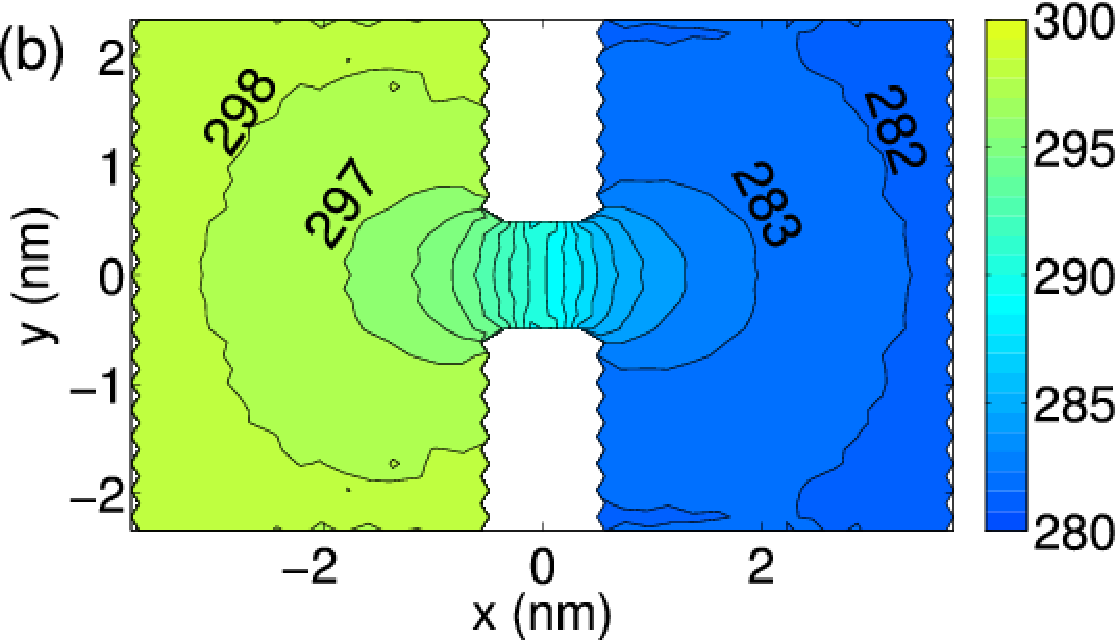
\includegraphics[width=.49\columnwidth]{pics/gf_fig8b.pdf}
 \end{center}
 \caption{(a) Illustration of a point contact in graphene. The leads (red and blue atoms) extend infinitely to the left and right, but the temperatures are determined self-consistently only for the center region (green atoms). (b) Self-consistent bath temperature profiles (K). The semi-infinite leads are at temperatures $T_L=300$ K and $T_R=280$ K. Phonon relaxation time $\tau=1/\gamma$ is set to $1$ ps. Figure (b) reprinted with publisher's permission from \citepub{gf}.}
 \label{fig:gf_fig8}
\end{figure}

The calculated temperature profile in the graphene point contact is plotted in Fig. \ref{fig:gf_fig8}(b) for lead temperatures $T_L=300$ K and $T_R=280$ K. In the considered geometry, there are no visible interference effects in temperature profiles. Quantum effects are observable in the slight asymmetry in temperature profiles at different sides of the junction: purely classical statistics would produce a fully symmetric temperature profile due to the linearity of the self-consistent equations for bath temperatures, as discussed in \citepub{gf}.

The same principles as outlined here for phonon transport can be directly applied to electron transport as well, when the equations of motion for lattice vibrations (Eq. \eqref{eq:th_eom1}) are replaced by the electronic ones (Eq. \eqref{eq:th_eom3}). In electron transport, the self-consistent baths are often referred to as voltage-temperature probes \cite{jacquet09}. Applications of voltage-temperature probe models for describing dissipation effects in electron transport have been so far limited only to one-dimensional geometries \cite{buttiker86,damato90,jacquet09,jacquet12}, although the model can account for wave dynamics, Joule heating as well as thermoelectric effects \cite{roy07} in complicated geometries. Recently, Bergfield \textit{et al.} used the model for investigating quantum temperature oscillations in electrically biased graphene \cite{bergfield15}. 

\subsection{Cavity-modified electromagnetic energy transfer}
\label{sec:results_cavity}

In 1946, Purcell \cite{purcell46} suggested that the emission of electromagnetic radiation from an oscillating dipole could be enhanced by placing the oscillator in a resonant cavity, which effectively increases the electromagnetic density of states and, therefore, the probability of spontaneous emission. The possibility to tune the rate of spontaneous emission was later demonstrated also experimentally \cite{hulet85}\cite{martini87} and is applied, e.g., in resonant cavity light-emitting diodes \cite{schubert92} to enhance the light emission from the active region.

Purcell effect raises the natural question of what are the conditions for similarly tuning the thermal conductance between electromagnetically coupled dielectric bodies. Unlike near-field enhancement of energy transfer, such cavity-tuning is expected to persist at large distances and could be applied, e.g., to (i) enhancing thermal coupling between dielectric bodies, allowing for efficient cooling of hot spots, or (ii) suppressing thermal coupling, preventing undesired propagation of heat.

\begin{figure}
 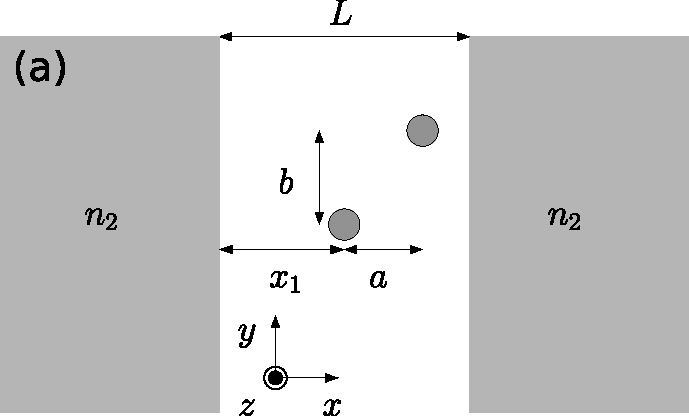
\includegraphics[width=.55\columnwidth]{pics/dipole_fig2.pdf}
 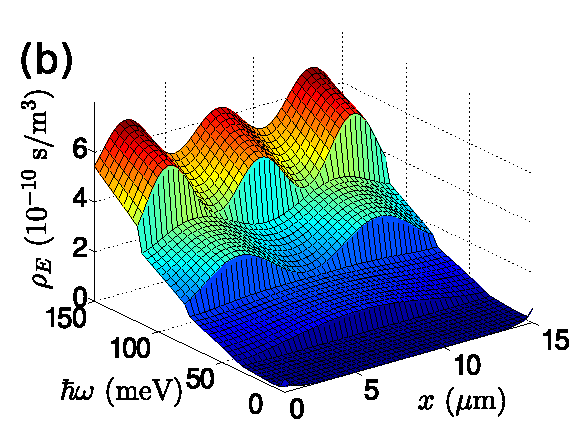
\includegraphics[width=.44\columnwidth]{pics/dipole_fig3a_mod.pdf}
 \caption{(a) Schematic illustration of two nanoparticles located in a mirror cavity of length $L$. One of the particles is located at the middle of the cavity and the position of the second particle is defined by parameters $a$ and $b$ as shown in the figure. The refractive index of the cavity walls is denoted by $n_2$. (b) Electromagnetic density of states as a function of position and energy for a cavity with $L=16$ $\upmu$m and $n_2=2+20i$. The lowest-frequency standing waves have cut-off energies 37.6 meV, 76.3 meV, and 115.1 meV. These modes can couple to the absorption resonance of SiC nanoparticles at $\hbar\omega_r=115.6$ meV. Figure reprinted with publisher's permission from \citepub{dipole}.}
\label{fig:gfm_dipole_system}
\end{figure}

The system studied in \citepub{dipole} is schematically depicted in Fig. \ref{fig:gfm_dipole_system}(a). Two SiC nanoparticles are located in a microcavity formed by two half-spaces with refractive index $n_2=2+20i$ and separated by distance $L$. Due to cavity confinement, the electromagnetic field forms standing waves in the cavity, which can be seen as ''stairs'' in the electromagnetic density of states shown in Fig. \ref{fig:gfm_dipole_system}(b). For $L=16$ $\upmu$m, the lowest-energy standing waves can be excited at 37.6 meV, 76.3 meV, and 115.1 meV. The length of the cavity $L=16$ $\upmu$m is chosen such that only these three low-energy modes can couple electromagnetically to the SiC nanoparticle resonances at 115.6 meV (see below). 

The radius of the nanoparticles is assumed to be $R=250$ nm and the relative dielectric constant $\varepsilon(\omega)$ of SiC is modeled by the Lorentz model \cite{mulet01,spitzer59}. The Clausius-Mossotti polarizabilities of the particles are given by
\begin{equation}
 \alpha^{\textrm{CM}}(\omega)= 4 \pi R^3 \frac{\varepsilon(\omega)-1}{\varepsilon(\omega)+2} \unitdyadic.
\end{equation}
The particles have strong absorption peaks at the phonon-polariton resonance energy $\hbar \omega_r=115.6$ meV corresponding to $\textrm{Re}[\varepsilon(\omega)]=-2$, which forces the interparticle energy transfer to be nearly monochromatic. As discussed above, only three lowest-energy standing waves can be excited in the $L=16$ $\upmu$m cavity at this frequency, and the coupling of the particles to the electromagnetic field therefore depends strongly on the positions of the particles.  

\begin{figure}
 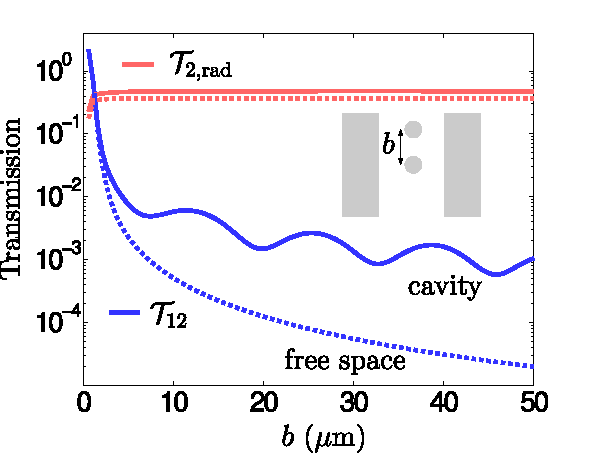
\includegraphics[width=.79\columnwidth]{pics/dipole_fig5.pdf}
 \caption{Energy transmission function $\ca{T}_{12}(\omega_r)$ between two SiC nanoparticles at the nanoparticle resonance frequency $\omega_r$ as a function of vertical separation $b$ (see the inset). The mirror cavity enhances the interparticle thermal conductance and gives rise to interference effects seen as conductance oscillations as a function of distance. The cavity also enhances the coupling between the environment and each dipole, as indicated by the larger dipole-environment transmission function $\ca{T}_{2,\textrm{rad}}(\omega_r)$ with mirror cavity (solid red line) than in free-space (dashed red line). Figure reprinted with publisher's permission from \citepub{dipole}.}
\label{fig:dipole_fig5}
\end{figure}

Figure \ref{fig:dipole_fig5} shows the dipole-dipole transmission $\ca{T}_{12}(\omega_r)$ and the dipole-environment transmission $\ca{T}_{2,\textrm{rad}}(\omega_r)$ at the resonance energy $\hbar\omega_r=115.6$ meV as a function of the vertical distance $b$. The interparticle transmission $\ca{T}_{12}(\omega_r)$ in the cavity (solid blue line) can be seen to exceed the free-space value (dashed blue line) at distances larger than $b\approx 2$ $\upmu$m. In addition, the transmission oscillates as a function of distance due to the interference between electromagnetic cavity modes. As shown in \citepub{dipole}, interparticle thermal conductance can be similarly enhanced also by placing the particles close to a SiC surface supporting surface phonon polaritons.

These results suggest that electromagnetic energy transfer rates between particles can be tuned by modifying the electromagnetic environment, in analogy with the Purcell tuning of radiative emission. Increasing the coupling to the electromagnetic field increases, however, also the thermal coupling to the environment, which may overshadow the interparticle energy transfer. Heat flow from the environment to the particles could be reduced by, e.g., cooling the cavity walls. 




\chapter{Outlook}


\section{Applications of linear Langevin equations}

\subsection{Coupling of models}

\subsection{Application to electron transport}


The same principles as outlined in Sec. \ref{sec:th_schb} for phonon transport can be directly applied to electron transport as well, when Langevin heat baths are replaced by electron baths. In this case, the self-consistent baths are often referred to as voltage-temperature probes \cite{jacquet09}. Previous applications of voltage-temperature probe models for describing dissipation effects in electron transport have been limited to one-dimensional geometries \cite{buttiker86,damato90,jacquet09,jacquet12}. Recently, Bergfield et al. used the model for investigating quantum temperature oscillations in graphene \cite{bergfield15}.

\section{Future applications for spectral heat current calculations}

\chapter{Conclusion and outlook}


Recent advances in manufacturing techniques have enabled controlling energy transfer in nanoscale structures. These advances have both improved the efficiency of existing device applications such as thermoelectric heat-to-electricity converters and spawned new applications such as heat-assisted magnetic recording. Releasing the full potential of thermal energy requires, however, a more thorough understanding of energy transfer and conversion in nanoscale.

% Control of charge transfer in small structures, electronics, has given rise to the Digital Revolution.

In this thesis, we have developed new computational methods and analysis procedures for investigating energy transfer in nanoscale systems.  We developed a mathematical expression for the spectral decomposition of the thermal current, used in conjunction with non-equilibrium molecular dynamics simulation to investigate non-linear phononic energy transfer at interfaces and in nanotubes. We also showed that Langevin theory and the Green's function solution of equations of motion can be used to determine phononic, photonic as well as electronic energy transfer rates using very similar calculation methods, unifying the mathematical treatment of different energy carriers. %The methods were applied along with existing methods to investigate phononic and photonic energy transfer. % deliver new physical insight into the complex energy-related processes taking place in nanoscale structures. 

Using non-equilibrium molecular dynamics, we showed that anharmonic phonon-phonon scattering at a material interface increases the interfacial conductance by providing a dissipation mechanism for evanescent waves and enabling multi-phonon energy transfer processes at the interface. As material interfaces typically form the major bottleneck for heat flow in electronic devices, such a detailed understanding of energy transfer might assist in designing better thermally conducting interfaces in future. We also provided numerical evidence that energy transfer in carbon nanotubes is partially ballistic even in micrometer-long tubes due to the long mean free paths at low vibrational frequencies, providing further support for the applicability of carbon nanotubes in thermal management. In silicon nanowires, periodic twinning with a suitably chosen twinning period was shown to strongly decrease the thermal conductivity, suggesting that the thermoelectric conversion efficiency of nanowires could be further increased by such nanostructuring. 

Green's function methods were used to investigate thermal conduction through point contacts in two-dimensional lattices, highlighting the importance of quantum statistics in determining the local temperature. For a point contact in graphene at room temperature, quantum statistical and classical calculations deliver, however, very similar temperature profiles, suggesting that the low-frequency modes (not affected by quantum statistics) are primarily responsible for energy transfer in such structures. Green's function solution of Langevin equations of motion was also applied to investigating electromagnetic energy transfer between polar nanoparticles in a mirror cavity, proposing the possibility to tune electromagnetic energy transfer rates by the modification of electromagnetic density of states. 

The spectral heat current formula developed in this thesis holds great promise for future investigations of energy transfer in nanoscale. Combined with the versatility of molecular dynamics simulations, the spectral decomposition can present a detailed picture of energy transfer processes in various systems, including, e.g., the interface between a solid and a liquid, important in applications such as hyperthermic treatment by heated nanoparticles. Determining the mean free paths is expected to provide theoretical supplement to experimental mean free path spectroscopy measurements and could also provide microscopic insight to the anomalous thermal conduction observed in low-dimensional systems.

Green's function modeling of energy transfer has a lot of potential due to its applicability to phononic, photonic as well as electronic systems. The method can account for quantum statistics, wave effects such as interference, and even carrier dissipation in terms of relaxation rates. Energy exchange between carriers, necessary in the modeling of, e.g., electronic generation of heat in nanoscale structures, could be flexibly modeled using the Green's function method by including an energy exchange term between the carriers in the thermal balance equations. At first order, this energy exchange is expected to be given by the product of the carrier-carrier coupling coefficient and the temperature difference between different systems.

\textbf{FINAL REMARKS ON FUTURE}

% Using NEMD, we investigated phononic energy transfer at an interface between two crystals, carbon nanotube, silicon nanowire with periodic twinning, and point contact in a two-dimensional lattice. 

% Short summary of results

% Outlook
% - Spectral analysis of energy current: liquids and gases, engineering of thermal conductivity in non-linear structures, new understanding of thermal rectification, investigation of one-dimensional thermal conduction, determining mean free paths in amorphous and crystalline materials
% - Green's function methods: self-consistent temperature calculation at interfaces, coupling of different models

\renewcommand{\bibname}{References}
\bibliographystyle{thesis_style}
%\bibliographystyle{../test}
\bibliography{../bibtex/biblio}{}

%\bibliographystyle{ieeetr}
%\bibliographystyle{../physrev}




\addpublication{K. S\"a\"askilahti, J. Oksanen, J. Tulkki, and S. Volz}{Role of anharmonic phonon scattering in the spectrally decomposed thermal conductance at planar interfaces}{Phys. Rev. B}{90, 134312}{October}{2014}{American Physical Society}{spectral}
% Add the dissertation author's contribution to that publication (the order can be interchanged with \adderrata).
%\addcontribution{The author did this and that}
% Add the errata of the publication, remove if there are none (the order can be interchanged with \addauthorscontribution).
%\adderrata{This is wrong}
% Add the publication pdf file, the filename is the parameter (must be the last).
\addpublicationpdf{articles/spectral_article.pdf}

\addpublication{K. S\"a\"askilahti, J. Oksanen, S. Volz, and J. Tulkki}{Frequency-dependent phonon mean free paths in carbon nanotubes from nonequilibrium molecular dynamics}{Phys. Rev. B}{91, 115426}{March}{2015}{American Physical Society}{cnt}
% Add the dissertation author's contribution to that publication (the order can be interchanged with \adderrata).
%\addcontribution{The author did this and that}
% Add the errata of the publication, remove if there are none (the order can be interchanged with \addauthorscontribution).
%\adderrata{This is wrong}
% Add the publication pdf file, the filename is the parameter (must be the last).
\addpublicationpdf{articles/cnt_article.pdf}


\addpublication{Shiyun Xiong, Yuriy A. Kosevich, K. S\"a\"askilahti, Yuxiang Ni, and Sebastian Volz}{Tunable thermal conductivity in silicon twinning superlattice nanowires}{Phys. Rev. B}{90, 195439}{November}{2014}{American Physical Society}{twinning}
% Add the dissertation author's contribution to that publication (the order can be interchanged with \adderrata).
%\addcontribution{The author did this and that}
% Add the errata of the publication, remove if there are none (the order can be interchanged with \addauthorscontribution).
%\adderrata{This is wrong}
% Add the publication pdf file, the filename is the parameter (must be the last).
\addpublicationpdf{articles/twinning_article.pdf}

\addpublication{K. S\"a\"askilahti, J. Oksanen, R.~P. Linna, and J. Tulkki}{Thermal conduction and interface effects in nanoscale Fermi-Pasta-Ulam conductors}{Phys. Rev. E}{86, 031107}{September}{2012}{American Physical Society}{fpu}
% Add the dissertation author's contribution to that publication (the order can be interchanged with \adderrata).
% \addcontribution{The author made the coffee.}
% Add the errata of the publication, remove if there are none (the order can be interchanged with \addauthorscontribution).
%\adderrata{This is wrong}
% Add the publication pdf file, the filename is the parameter (must be the last).
\addpublicationpdf{articles/fpu_article.pdf}

\addpublication{K. S\"a\"askilahti, J. Oksanen, R.~P. Linna, and J. Tulkki}{Phonon interference and anharmonicity effects in nanoconstrictions}{AIP Conf. Proc.}{1506, 15}{December}{2012}{American Physical Society}{fpu2}
% \addcontribution{The author made the coffee.}.
% Add the dissertation author's contribution to that publication (the order can be interchanged with \adderrata).
%\addcontribution{The author made the coffee.}
% Add the errata of the publication, remove if there are none (the order can be interchanged with \addauthorscontribution).
%\adderrata{This is wrong}
% Add the publication pdf file, the filename is the parameter (must be the last).
\addpublicationpdf{articles/fpu_article2b.pdf}

\addpublication{K. S\"a\"askilahti, J. Oksanen, and J. Tulkki}{Thermal balance and quantum heat transport in nanostructures thermalized by local Langevin heat baths}{Phys. Rev. E}{88, 012128}{July}{2013}{American Physical Society}{gf}
% Add the dissertation author's contribution to that publication (the order can be interchanged with \adderrata).
%\addcontribution{The author did this and that}
% Add the errata of the publication, remove if there are none (the order can be interchanged with \addauthorscontribution).
%\adderrata{This is wrong}
% Add the publication pdf file, the filename is the parameter (must be the last).
\addpublicationpdf{articles/gf_article.pdf}

\addpublication{K. S\"a\"askilahti, J. Oksanen, and J. Tulkki}{Quantum Langevin equation approach to electromagnetic energy transfer between dielectric bodies in an inhomogeneous environment}{Phys. Rev. B}{89, 134301}{April}{2014}{American Physical Society}{dipole}
% Add the dissertation author's contribution to that publication (the order can be interchanged with \adderrata).
%\addcontribution{The author did this and that}
% Add the errata of the publication, remove if there are none (the order can be interchanged with \addauthorscontribution).
%\adderrata{This is wrong}
% Add the publication pdf file, the filename is the parameter (must be the last).
\addpublicationpdf{articles/dipole_article.pdf}


\end{document}